\documentclass[12pt,openany,oneside,a4paper,chapter=TITLE,english,brazil]{abntex2}

\usepackage{fontspec}
\setmainfont{texgyretermes}[Extension=.otf,UprightFont=*-regular,BoldFont=*-bold,ItalicFont=*-italic,BoldItalicFont=*-bolditalic]
\setmonofont{DejaVuSansMono}[Extension=.ttf,Scale=0.82,BoldFont=*-Bold,ItalicFont=*-Oblique,BoldItalicFont=*-BoldOblique]
\usepackage{newunicodechar}
\newunicodechar{↔}{\ensuremath{\leftrightarrow}}
\newunicodechar{∥}{\ensuremath{\parallel}}
\usepackage{xcolor}
\usepackage{graphicx}
\graphicspath{{../}}
\usepackage{tabularx,array,booktabs}
\usepackage{placeins}
\usepackage{fvextra}
\RecustomVerbatimEnvironment{verbatim}{Verbatim}{breaklines,breakanywhere,fontsize=\footnotesize,frame=single,framesep=2mm}
\usepackage{mdframed}
\usepackage{xurl}
\urlstyle{same}
\usepackage{microtype}

\renewcommand{\ABNTEXchapterfont}{\rmfamily\bfseries\raggedright\hyphenpenalty=10000\exhyphenpenalty=10000}
\renewcommand{\ABNTEXsectionfont}{\rmfamily\bfseries\raggedright\hyphenpenalty=10000\exhyphenpenalty=10000}
\renewcommand{\ABNTEXsubsectionfont}{\rmfamily}
\renewcommand{\ABNTEXsubsubsectionfont}{\rmfamily\itshape}
\makeatletter
\renewcommand{\ABNTEXchapterupperifneeded}[1]{%
  \ifthenelse{\boolean{abntex@innonumchapter}\OR\boolean{abntex@apendiceousecao}}{}{\raggedright}%
  \ifthenelse{\boolean{ABNTEXupperchapter}}{\MakeTextUppercase{#1}}{#1}}
\makeatother
\providecommand{\tightlist}{\setlength{\itemsep}{0pt}\setlength{\parskip}{0pt}}
\providecommand{\pandocbounded}[1]{#1}

\newcommand{\quadroname}{Quadro}
\newcommand{\listofquadrosname}{Lista de quadros}
\newfloat[chapter]{quadro}{loq}{\quadroname}
\newlistof{listofquadros}{loq}{\listofquadrosname}
\newlistentry{quadro}{loq}{0}
\setfloatadjustment{quadro}{\centering}
\counterwithout{quadro}{chapter}
\renewcommand{\cftquadroname}{\quadroname\space}
\renewcommand*{\cftquadroaftersnum}{\hfill--\hfill}
\setfloatlocations{quadro}{!htbp}

\renewcommand{\topfraction}{0.9}
\renewcommand{\bottomfraction}{0.8}
\renewcommand{\textfraction}{0.07}
\renewcommand{\floatpagefraction}{0.8}
\setcounter{topnumber}{3}
\setcounter{bottomnumber}{2}
\setcounter{totalnumber}{4}
\makeatletter
\setlength{\@fptop}{0pt}
\setlength{\@fpsep}{12pt}
\setlength{\@fpbot}{0pt plus 1fil}
\makeatother

\newenvironment{referenciasabnt}
  {\begin{flushleft}\SingleSpacing\setlength{\parindent}{0pt}\setlength{\parskip}{\baselineskip}}
  {\end{flushleft}}

\titulo{Livro do aluno: Cilium BGP, Gateway API e tenants híbridos: guia de estudo e prática}
\autor{Reinaldo Saraiva}
\local{Teresina}
\data{2026}
\preambulo{Edição 2.8. Público-alvo: estudantes de Kubernetes, redes e Cilium que já conhecem o vocabulário básico de IP e roteamento.}

\makeatletter
\hypersetup{
  pdftitle={\@title},
  pdfauthor={\@author},
  pdfsubject={Laboratório Kubernetes, Cilium e BGP},
  pdfkeywords={Cilium}{BGP}{Gateway API}{Kubernetes}{eBPF},
  colorlinks=true,
  linkcolor=black,
  citecolor=black,
  urlcolor=blue!50!black,
  bookmarksdepth=4
}
\makeatother

\setlrmarginsandblock{3cm}{2cm}{*}
\setulmarginsandblock{3cm}{2cm}{*}
\checkandfixthelayout
\setlength{\parindent}{1.3cm}
\setlength{\parskip}{0.2cm}
\setlength{\emergencystretch}{5em}
\tolerance=1000

\begin{document}
\selectlanguage{brazil}
\renewcommand{\listfigurename}{Lista de figuras}
\frenchspacing

\imprimircapa
\imprimirfolhaderosto

\pretextualchapter{Apresentação}
\begin{mdframed}[linewidth=0.6pt,innertopmargin=6pt,innerbottommargin=6pt]
\small
\textbf{Objetivo do guia}

Ao final do guia, a pessoa estudante deve conseguir:

\begin{itemize}
\tightlist
\item
  explicar o que o Cilium anuncia por BGP e como o tráfego chega a um
  pod ou a uma VIP anycast;
\item
  validar um Gateway HTTP, TCP e UDP exposto por VIP e ler decisões de
  autorização na borda e no datapath;
\item
  distinguir autorização por identidade de autorização por endereço em
  tenants com pods e VMs;
\item
  interpretar, como evidência histórica, os estudos avançados dos
  módulos 12 a 17.
\end{itemize}
\end{mdframed}

Este livro acompanha um laboratório de redes Kubernetes construído com Cilium,
BGP e um fabric de data center simulado em contêineres. Ele foi escrito para
quem já conhece o básico de IP e roteamento e quer entender, com evidência
medida, o que o Cilium faz e onde ele para.

O guia tem 17 módulos, organizados em quatro blocos:

\begin{itemize}
\tightlist
\item
  \textbf{Módulos 1 a 5, fundamentos no lab \texttt{k01}:} o que o Cilium anuncia por BGP, VIP anycast, dual-stack IPv6, falhas e escala. São exercícios práticos.
\item
  \textbf{Módulos 6 a 11, plataforma no sandbox \texttt{p003-{}\allowbreak{}gw}:} Gateway API, autorização externa, WireGuard, isolamento de tenants, Multi-Pool IPAM e tenants híbridos com VMs OpenStack. Também são práticos.
\item
  \textbf{Módulos 12 e 13, estudos históricos:} nós reais em nuvem e a trilha P004, que compara o Cilium com OVN-Kubernetes, FRR e EVPN para VMs KubeVirt.
\item
  \textbf{Módulos 14 a 17, estudos avançados P005 a P008:} 32 estudos sobre borda eBGP, datapath eBPF, multicluster, SRv6, segurança em tempo de execução e desempenho, todos concluídos com PASS.
\end{itemize}

Os módulos 12 a 17 são leitura: não exigem acesso às infraestruturas que
descrevem. Nenhum módulo mede desempenho de hardware de produção; os números
vêm de um laboratório em contêineres e valem como comparação entre
configurações, não como valor absoluto.

Os códigos que aparecem ao longo do texto, como \texttt{P004-{}\allowbreak{}S003}, \texttt{E27} e \texttt{G07},
identificam trilhas, sessões, estudos e critérios do projeto; o Quadro 2, na
Introdução, explica como lê-los. As citações seguem o sistema autor-data da
ABNT NBR 10520:2023, e as referências, a ABNT NBR 6023:2018.


\pdfbookmark[0]{\listfigurename}{lof}
\listoffigures*
\cleardoublepage
\pdfbookmark[0]{\listofquadrosname}{loq}
\listofquadros*
\cleardoublepage
\pdfbookmark[0]{\listtablename}{lot}
\listoftables*
\cleardoublepage
\pdfbookmark[0]{\contentsname}{toc}
\tableofcontents*
\cleardoublepage

\textual
\OnehalfSpacing

\chapter*{Introdução}
\addcontentsline{toc}{chapter}{Introdução}
\markboth{Introdução}{Introdução}

Esta introdução apresenta o Cilium e o vocabulário do guia, discute quando faz
sentido usá-lo e reúne o que a pessoa estudante precisa antes do Módulo 1:
objetivos, regras de segurança, onde cada comando roda, o mapa dos
laboratórios e a pergunta central do guia.

\section*{O que é o Cilium}\label{o-que-uxe9-o-cilium}
\addcontentsline{toc}{section}{O que é o Cilium}

O Cilium é um software de código aberto que fornece rede, segurança e
observabilidade para cargas em contêineres, principalmente no Kubernetes
(Cilium Authors, 2026d). No Kubernetes, ele atua como plugin CNI: cria a
interface de rede de cada pod, atribui endereços e encaminha o tráfego entre
pods, nós e o mundo externo.

A base do Cilium é o eBPF, tecnologia que executa programas verificados e
isolados dentro do kernel Linux, sem alterar o código do kernel nem carregar
módulos (eBPF Foundation, {[}2026{]}). Em vez de depender de longas cadeias de
regras do \texttt{iptables}, o Cilium anexa programas eBPF aos pontos por onde os
pacotes passam e guarda o estado em mapas eBPF. É por isso que, no Módulo 4, o
datapath continua encaminhando enquanto o agente reinicia.

Três ideias do Cilium aparecem em quase todos os módulos:

\begin{itemize}
\tightlist
\item
  \textbf{identidade em vez de endereço:} o Cilium atribui uma identidade de segurança a cada conjunto de labels e aplica as políticas sobre ela, não sobre o IP (Cilium Authors, 2026d); o Módulo 11 mostra a consequência prática quando um IP muda de dono;
\item
  \textbf{um agente por nó:} o \texttt{cilium-{}\allowbreak{}agent} programa o datapath do nó e, com o BGP Control Plane habilitado, mantém as sessões BGP daquele nó (Cilium Authors, 2026b);
\item
  \textbf{funções integradas:} balanceamento de Services sem o \texttt{kube-{}\allowbreak{}proxy}, Gateway API com Envoy embutido, criptografia transparente com WireGuard e observabilidade de fluxos com o Hubble vêm do mesmo projeto (Cilium Authors, 2026d).
\end{itemize}

O Cilium foi criado pela Isovalent, entrou na Cloud Native Computing
Foundation (CNCF) como projeto incubado em outubro de 2021 e foi graduado em
outubro de 2023 (Cloud Native Computing Foundation, 2023). A versão usada no
laboratório, a 1.20, exige kernel Linux 5.10 ou superior, ou equivalente como o
4.18 do RHEL 8.10 (Cilium Authors, 2026g).

\section*{A Isovalent e o ecossistema comercial}\label{a-isovalent-e-o-ecossistema-comercial}
\addcontentsline{toc}{section}{A Isovalent e o ecossistema comercial}

A Isovalent é a empresa que criou o Cilium e que vende distribuições
comerciais do projeto, com suporte e recursos adicionais. Em abril de 2024, a
Cisco concluiu a aquisição da Isovalent (Isovalent, 2024). O Cilium segue como
projeto graduado da CNCF, com mantenedores de várias empresas (Cloud Native
Computing Foundation, 2023).

Este guia usa apenas o Cilium de código aberto (OSS). A sigla \textbf{INV}, que
aparece no Módulo 13, designa o \emph{Isovalent Networking for Virtualization},
oferta comercial voltada a máquinas virtuais no Kubernetes (Isovalent, 2026).
A trilha P004 compara as capacidades que essa oferta anuncia com o que se
obtém combinando projetos abertos; ela não testa o produto comercial.

\section*{Termos principais}\label{termos-principais}
\addcontentsline{toc}{section}{Termos principais}

O Quadro 1 reúne os termos técnicos usados ao longo do guia, e o Quadro 2,
os códigos que identificam trilhas, sessões, estudos e critérios do projeto.
Vale consultá-los sempre que um termo ou código parecer obscuro.

\begin{quadro}[!htbp]
\caption{Termos principais usados no guia}
\footnotesize
\begin{tabularx}{\textwidth}{|>{\raggedright\arraybackslash\hsize=0.519\hsize}X|>{\raggedright\arraybackslash\hsize=1.481\hsize}X|}
\hline
\textbf{Termo} & \textbf{Significado neste laboratório} \\
\hline
\textbf{eBPF} & tecnologia do kernel Linux que executa programas verificados e isolados
em pontos do caminho dos pacotes \\
\hline
\textbf{CNI} & interface pela qual o Kubernetes pede a um plugin de rede que conecte
cada pod; o Cilium é um plugin CNI \\
\hline
\textbf{datapath} & conjunto de programas eBPF e mapas que encaminham, filtram e balanceiam
os pacotes no nó \\
\hline
\textbf{XDP e TC/TCX} & pontos do kernel onde o Cilium anexa programas eBPF: XDP na chegada do
pacote à interface, TC/TCX na pilha de rede \\
\hline
\textbf{identidade} & número que o Cilium atribui a um conjunto de labels; as políticas são
avaliadas sobre a identidade, não sobre o IP \\
\hline
\textbf{speaker} & o agente Cilium em um nó, que mantém a sessão BGP daquele nó \\
\hline
\textbf{PodCIDR} & bloco de IP reservado para pods de um nó; \texttt{/\allowbreak{}24} IPv4
por nó no IPAM \texttt{kubernetes} \\
\hline
\textbf{VIP} & endereço de serviço anunciado como \texttt{/\allowbreak{}32} por vários
nós \\
\hline
\textbf{native routing} & o pacote do pod viaja com o IP real do pod, roteado pelo fabric, sem
encapsulamento \\
\hline
\textbf{overlay VXLAN} & o pacote do pod viaja encapsulado em UDP entre os nós; o fabric vê
apenas os IPs dos nós \\
\hline
\textbf{ECMP} & vários próximos saltos equivalentes para o mesmo prefixo \\
\hline
\textbf{GR} & Graceful Restart: o vizinho mantém as rotas enquanto a sessão BGP
reinicia (Sangli et al., 2007) \\
\hline
\textbf{Gateway API} & recursos \texttt{Gateway}, \texttt{HTTPRoute}, \texttt{TCPRoute},
\texttt{UDPRoute} implementados pelo Cilium com Envoy (Kubernetes SIG
Network, 2026) \\
\hline
\textbf{Envoy} & proxy L7 que o Cilium executa no nó para a Gateway API, as políticas
HTTP e o \texttt{Cilium\allowbreak{}Envoy\allowbreak{}Config} \\
\hline
\textbf{ExternalAuth} & filtro do Gateway API que consulta um serviço externo antes de
encaminhar a requisição \\
\hline
\textbf{CNP} & \texttt{Cilium\allowbreak{}Network\allowbreak{}Policy};
\texttt{from\allowbreak{}Endpoints} seleciona por label,
\texttt{from\allowbreak{}CIDR} por endereço (Cilium Authors, 2026h) \\
\hline
\textbf{Multi-Pool} & IPAM do Cilium em que cada nó recebe blocos de um
\texttt{Cilium\allowbreak{}Pod\allowbreak{}IPPool}, com
\texttt{mask\allowbreak{}Size} configurável (Cilium Authors, 2026e) \\
\hline
\textbf{Hubble} & camada de observabilidade do Cilium que registra fluxos L3/L4 e L7 \\
\hline
\textbf{WireGuard} & protocolo de túnel cifrado que o Cilium usa para criptografar o tráfego
entre nós \\
\hline
\textbf{VRF} & tabela de roteamento isolada; permite que tenants diferentes usem o
mesmo CIDR \\
\hline
\textbf{EVPN} & família do BGP que anuncia redes L2 (Type 2) e prefixos IP (Type 5) de
tenants, em geral sobre VXLAN \\
\hline
\textbf{SRv6} & roteamento por segmentos sobre IPv6; aqui, usado como VPN L3
(\texttt{End.\allowbreak{}DT4}/\texttt{End.\allowbreak{}DT6}) sem VXLAN \\
\hline
\textbf{KubeVirt} & extensão que executa máquinas virtuais como recursos do Kubernetes \\
\hline
\textbf{OVN-Kubernetes} & plugin CNI baseado em OVN e OVS, usado como alternativa aberta no Módulo
13 \\
\hline
\textbf{SG} & Security Group do Neutron, o firewall stateful da porta de uma VM \\
\hline
\textbf{RX morto} & a VM envia mas não recebe; limitação de KVM aninhado em container \\
\hline
\end{tabularx}
\fonte{elaborado pelo autor (2026).}
\end{quadro}

\begin{quadro}[!htbp]
\caption{Códigos do projeto usados no guia}
\footnotesize
\begin{tabularx}{\textwidth}{|>{\raggedright\arraybackslash\hsize=0.807\hsize}X|>{\raggedright\arraybackslash\hsize=1.194\hsize}X|>{\raggedright\arraybackslash\hsize=0.999\hsize}X|}
\hline
\textbf{Código} & \textbf{Significado} & \textbf{Exemplo} \\
\hline
\texttt{P001}--\texttt{P008} & trilha (plano de trabalho) do projeto & \texttt{P004}: DCI, OVN-Kubernetes e KubeVirt \\
\hline
\texttt{S001}, \texttt{S002}\ldots{} & sessão de execução dentro de uma trilha & \texttt{P004-{}\allowbreak{}S003} \\
\hline
\texttt{E01}--\texttt{E41} & estudo experimental & \texttt{E27}: BIG TCP com \texttt{netkit} \\
\hline
Onda e Braço & grupo de estudos executados juntos e frente de trabalho dentro da onda & Onda 2, Braço A \\
\hline
\texttt{G00}--\texttt{G09} & gate: critério que a trilha precisa cumprir para ser fechada & \texttt{G07}: critérios de aceite do INV \\
\hline
letras e número (\texttt{M01}, \texttt{K02}, \texttt{X05},
\texttt{V07-{}\allowbreak{}A}, \texttt{C04}, \texttt{T07}, \texttt{A08},
\texttt{I01}) & caso de teste dentro de uma matriz & \texttt{K02}: live migration no OVN-Kubernetes \\
\hline
\textbf{PASS} & sessão ou estudo concluído com todos os critérios atendidos & P005-S001 concluída com PASS \\
\hline
\texttt{R3}, \texttt{R6} & regras invariantes do laboratório & \texttt{R6=\allowbreak{}0}: nenhuma rota BGP instalada na tabela
\texttt{main} do kernel \\
\hline
\texttt{INV-{}\allowbreak{}Po\allowbreak{}C-{}\allowbreak{}01}--\texttt{INV-{}\allowbreak{}Po\allowbreak{}C-{}\allowbreak{}06} & critérios de aceite para uma prova de conceito do INV & Módulo 13.4 \\
\hline
\texttt{L1}--\texttt{L8} & lições operacionais & Apêndice A \\
\hline
\end{tabularx}
\fonte{elaborado pelo autor (2026).}
\end{quadro}

\section*{Quando usar e quando não usar o Cilium}\label{quando-usar-e-quando-nuxe3o-usar-o-cilium}
\addcontentsline{toc}{section}{Quando usar e quando não usar o Cilium}

Não existe resposta universal. O Quadro 3 resume o que os estudos deste guia
mostraram a favor e contra o Cilium, com o módulo em que cada evidência
aparece.

\begin{quadro}[!htbp]
\caption{Situações a favor e contra o Cilium, segundo os estudos do guia}
\footnotesize
\begin{tabularx}{\textwidth}{|>{\raggedright\arraybackslash\hsize=1.259\hsize}X|>{\raggedright\arraybackslash\hsize=1.024\hsize}X|>{\raggedright\arraybackslash\hsize=0.717\hsize}X|}
\hline
\textbf{Situação} & \textbf{Indicação} & \textbf{Evidência no guia} \\
\hline
Política de rede por identidade, inclusive em L7 & o Cilium é forte candidato & Módulos 9 e 11 \\
\hline
Anunciar PodCIDRs e VIPs de Service por BGP a um fabric físico & o BGP Control Plane do Cilium atende & Módulos 1 a 5 \\
\hline
Observar fluxos L3 a L7 sem sidecar & o Cilium com o Hubble atende & Módulo 14 (\texttt{E25}) \\
\hline
Gateway API, criptografia e balanceamento no mesmo componente & o Cilium reduz o número de peças & Módulos 6 a 8 \\
\hline
VRF, CIDR sobreposto ou EVPN na interface primária do pod & o Cilium OSS não atende; o OVN-Kubernetes atendeu & Módulo 13 (\texttt{V07-{}\allowbreak{}A}, \texttt{C-{}\allowbreak{}neg},
\texttt{K01}) \\
\hline
Live migration de VM KubeVirt preservando IP e sessões & o Cilium OSS troca o IP; o OVN-Kubernetes preservou & Módulo 13 (\texttt{V05}, \texttt{K02}) \\
\hline
Aprender rotas BGP no kernel, limitar prefixos ou usar BFD & manter essas funções no roteador de borda & Módulos 4 e 14 (\texttt{E10}, \texttt{E11}) \\
\hline
Kernel Linux anterior ao 5.10 (exceto equivalentes, como o 4.18 do RHEL
8.10) & o Cilium 1.20 não é suportado & requisitos do Cilium 1.20 \\
\hline
Apenas conectividade básica entre pods, sem política nem integração BGP & um CNI mais simples pode bastar & --- \\
\hline
\end{tabularx}
\fonte{elaborado pelo autor (2026).}
\end{quadro}

Em resumo, o Cilium é a escolha natural quando política por identidade,
observabilidade e integração BGP com o fabric são requisitos. Quando o
requisito central é multi-tenancy L3 com VRF e CIDR sobreposto para VMs, os
resultados do Módulo 13 apontam para o OVN-Kubernetes ou para uma oferta
comercial, a ser avaliada pelos critérios \texttt{INV-{}\allowbreak{}Po\allowbreak{}C-{}\allowbreak{}01} a \texttt{INV-{}\allowbreak{}Po\allowbreak{}C-{}\allowbreak{}06}.

\section*{Objetivos de aprendizagem}\label{objetivos-de-aprendizagem}
\addcontentsline{toc}{section}{Objetivos de aprendizagem}

\begin{itemize}
\tightlist
\item
  explicar a diferença entre sessão BGP, rota anunciada e encaminhamento de um pacote;
\item
  distinguir PodCIDR agregado, VIP de serviço e bloco Multi-Pool \texttt{/\allowbreak{}32};
\item
  expor um Gateway HTTP, TCP e UDP por uma VIP anunciada por BGP e provar cada listener com controle negativo;
\item
  ler uma decisão allow/deny/absent do ExternalAuth e reconhecer fail-closed;
\item
  verificar em captura se um tráfego está cifrado, encapsulado ou em claro;
\item
  provar isolamento de tenant em três controles diferentes: rede, borda e configuração;
\item
  explicar por que autorização por label não vaza no reuso de IP e por que autorização por CIDR vaza;
\item
  registrar separadamente a saída observada e a expectativa do roteiro;
\item
  interpretar os resultados de P004 (DCI/OVN/FRR/EVPN, OVN-Kubernetes + KubeVirt, casos cruzados e Braços Cilium A/B + KubeVirt, com todos os gates \texttt{G00–G09} concluídos), sem confundi-los com a trilha básica do Cilium.
\end{itemize}

\section*{Regras de segurança}\label{regras-de-seguranuxe7a}
\addcontentsline{toc}{section}{Regras de segurança}

\begin{itemize}
\tightlist
\item
  Os exercícios da pessoa estudante são de leitura e de requisição HTTP/TCP/UDP. Mutação é tarefa do instrutor e está marcada como tal.
\item
  Não use \texttt{kubectl delete}, \texttt{kubectl drain}, \texttt{docker stop}, \texttt{clab destroy} ou o script de teardown como parte deste roteiro.
\item
  Nunca dependa do contexto implícito do \texttt{kubectl}. Cada comando traz \texttt{-{}\allowbreak{}-{}\allowbreak{}kubeconfig} e \texttt{-{}\allowbreak{}-{}\allowbreak{}context}.
\item
  O cluster \texttt{k01} é a referência histórica protegida. Os estudos P003 rodam em um segundo cluster, o sandbox \texttt{p003-{}\allowbreak{}gw}. Antes de qualquer comando no sandbox, confirme o UID do cluster com o valor entregue pelo instrutor.
\item
  Se \texttt{127.\allowbreak{}0.\allowbreak{}0.\allowbreak{}1:\allowbreak{}18081} já responder no seu computador, existe um túnel ativo. Reutilize-o.
\item
  O módulo 13 é somente leitura de evidências históricas: não traz comandos interativos para DCI, OVN-Kubernetes ou KubeVirt e não pede acesso à VM atual.
\end{itemize}

\section*{Onde um comando roda}\label{onde-um-comando-roda}
\addcontentsline{toc}{section}{Onde um comando roda}

\begin{quadro}[!htbp]
\caption{Rótulos que indicam onde cada comando roda}
\footnotesize
\begin{tabularx}{\textwidth}{|>{\raggedright\arraybackslash\hsize=0.809\hsize}X|>{\raggedright\arraybackslash\hsize=1.191\hsize}X|}
\hline
\textbf{Rótulo} & \textbf{Significado} \\
\hline
\textbf{Mac} & computador da pessoa estudante \\
\hline
\textbf{vm-cilium} & sessão SSH no host Linux do laboratório \\
\hline
\textbf{container} & comando precedido por \texttt{sudo docker exec} na vm-cilium \\
\hline
\textbf{Kubernetes k01} & \texttt{sudo kubectl -{}\allowbreak{}-{}\allowbreak{}kubeconfig "\$K01\_\allowbreak{}KUBECONFIG" -{}\allowbreak{}-{}\allowbreak{}context kind-{}\allowbreak{}k01} \\
\hline
\textbf{Kubernetes sandbox} & \texttt{sudo kubectl -{}\allowbreak{}-{}\allowbreak{}kubeconfig "\$STUDY\_\allowbreak{}KUBECONFIG" -{}\allowbreak{}-{}\allowbreak{}context kind-{}\allowbreak{}p003-{}\allowbreak{}gw} \\
\hline
\textbf{testbed OpenStack} & \texttt{sudo docker exec -{}\allowbreak{}i \textless{}container-{}\allowbreak{}do-{}\allowbreak{}testbed\textgreater{} bash}
e, dentro dele, \texttt{openstack} \\
\hline
\end{tabularx}
\fonte{elaborado pelo autor (2026).}
\end{quadro}

Defina as variáveis uma vez por sessão na \textbf{vm-cilium}. Os valores abaixo são
os do laboratório de referência; use os que o instrutor entregar:

\begin{verbatim}
export LAB_DIR="${LAB_DIR:-/opt/poc-k8s-fabric}"
export K01_KUBECONFIG="${K01_KUBECONFIG:-/root/.kube/k01-rebuild.config}"
export STUDY_KUBECONFIG="${STUDY_KUBECONFIG:-/root/.kube/p003-gw.config}"
export STUDY_CLUSTER_UID="${STUDY_CLUSTER_UID:-<uid-entregue-pelo-instrutor>}"
k01() { sudo kubectl --kubeconfig "$K01_KUBECONFIG" --context kind-k01 "$@"; }
ks()  { sudo kubectl --kubeconfig "$STUDY_KUBECONFIG" --context kind-p003-gw "$@"; }
C1="sudo docker exec clab-poc-k8s-kind-client-ext"
C2="sudo docker exec clab-p003-gw-fabric-client"
UID_NOW="$(ks get namespace kube-system -o jsonpath='{.metadata.uid}')"
test "$UID_NOW" = "$STUDY_CLUSTER_UID" && echo "sandbox OK"
\end{verbatim}

Se o teste de UID falhar, pare. Um \texttt{kubectl} no cluster errado invalida o
exercício e pode alterar a referência.

\section*{Mapa dos laboratórios}\label{mapa-dos-laboratuxf3rios}
\addcontentsline{toc}{section}{Mapa dos laboratórios}

\begin{figure}[!htbp]
\caption{Visão geral do laboratório dentro da vm-cilium}
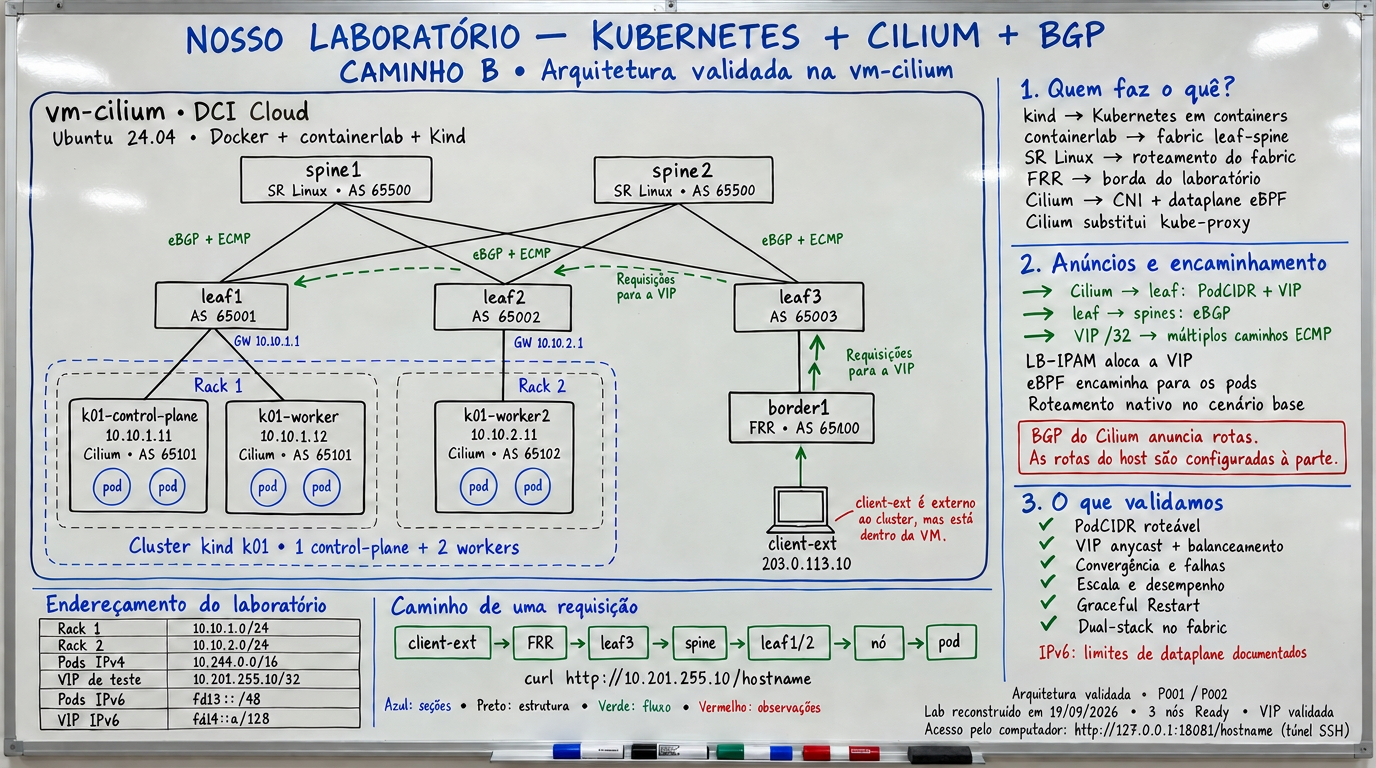
\includegraphics[width=\textwidth,height=0.72\textheight,keepaspectratio]{diagramas/05-laboratorio-vm-cilium-quadro-branco-v2.png}
\fonte{elaborada pelo autor (2026).}
\end{figure}

Os exercícios práticos dos módulos 1--11 usam os ambientes documentados nas
linhas abaixo. O módulo 12 é leitura de um estudo com infraestrutura em nuvem
que não faz parte da aula; o módulo 13 lê resultados históricos completos da
trilha P004 (DCI, OVN-Kubernetes + EVPN, casos cruzados e Braços Cilium A/B +
KubeVirt). O Quadro 5 distingue esses estudos dos ambientes usados nos exercícios:

\begin{quadro}[!htbp]
\caption{Ambientes e estudos documentados no guia}
\footnotesize
\begin{tabularx}{\textwidth}{|>{\raggedright\arraybackslash\hsize=0.812\hsize}X|>{\raggedright\arraybackslash\hsize=1.141\hsize}X|>{\raggedright\arraybackslash\hsize=1.019\hsize}X|>{\raggedright\arraybackslash\hsize=1.027\hsize}X|}
\hline
\textbf{Ambiente} & \textbf{Componentes} & \textbf{Versões} & \textbf{Papel} \\
\hline
\textbf{Lab de referência \texttt{k01}} & 2 spines + 3 leaves SR Linux, \texttt{border1} FRR,
\texttt{client-{}\allowbreak{}ext}, kind com 3 nós & SR Linux 25.3.2, FRR 8.4.1, Kubernetes v1.35.0, Cilium 1.20.1 & Módulos 1 a 5; protegido, somente leitura \\
\hline
\textbf{Sandbox \texttt{p003-{}\allowbreak{}gw}} & segundo fabric containerlab + kind com 3 nós + cliente
\texttt{198.\allowbreak{}19.\allowbreak{}0.\allowbreak{}10} & Cilium 1.20.2, Gateway API 1.6.1 (CRDs standard + experimental) & Módulos 6 a 11; onde o instrutor muda configuração \\
\hline
\textbf{Testbed OpenStack} & DevStack em container (Neutron OVS, qrouter, qdhcp, SG) & neutron 34.x, cirros 0.6.0 & Módulo 11; VMs do tenant \\
\hline
\textbf{VM em KVM real} & \texttt{qemu} no host ligado ao \texttt{br-{}\allowbreak{}int} do
testbed por um par veth & cirros 0.6.0 & Módulo 11, caso C5 \\
\hline
\textbf{Estudo histórico de nós reais na nuvem} & 3 VMs na nuvem, cluster \texttt{kubeadm} e FRR na mesma VPC & Kubernetes 1.35.2, Cilium 1.20.1 & Módulo 12; leitura, infraestrutura fora da aula \\
\hline
\textbf{Réplica DCI (\texttt{P004-{}\allowbreak{}S002})} & \texttt{labctl dci}: OVN 26.03.3, 1 central, 2 chassis, 2 gateways, FRR
multi-VRF e cliente AS 200 & Linux VRFs nos gateways; EVPN Type 5 (\texttt{M01–M03}, \texttt{X05}) & Módulo 13.1; leitura de resultados históricos (\texttt{labctl dci down}
após os ensaios) \\
\hline
\textbf{Plano OVN-Kubernetes + Fabric EVPN
(\texttt{P004-{}\allowbreak{}S003} e \texttt{S004})} & \texttt{labctl evpn-{}\allowbreak{}fabric} + \texttt{labctl ovnk}: kind
3 nós + \texttt{ovnk-{}\allowbreak{}evpn-{}\allowbreak{}peer} + KubeVirt
\texttt{/\allowbreak{}dev/\allowbreak{}kvm} & OVN-Kubernetes v1.4.0, KubeVirt v1.9.0, \texttt{frr-{}\allowbreak{}k8s}
v0.0.21/v0.0.27 & Módulo 13.2; leitura de resultados históricos (\texttt{K01–K04},
\texttt{X01–X04}, \texttt{X06–X07}) \\
\hline
\textbf{Braços Cilium A e B + KubeVirt
(\texttt{P004-{}\allowbreak{}S005} a \texttt{S008})} & \texttt{p003-{}\allowbreak{}gw} + KubeVirt
\texttt{/\allowbreak{}dev/\allowbreak{}kvm} +
\texttt{Daemon\allowbreak{}Set/\allowbreak{}frr-{}\allowbreak{}node} (no
Braço B sob \texttt{R6=\allowbreak{}0}) & Cilium 1.20.2, KubeVirt v1.9.0, FRR 10.7.1
(\texttt{table-{}\allowbreak{}map RM-{}\allowbreak{}NO-{}\allowbreak{}KERNEL}) & Módulos 13.3 e 13.4; leitura de resultados históricos (\texttt{V00–V09},
\texttt{G01}, \texttt{G02}, \texttt{G06–G08}) \\
\hline
\end{tabularx}
\fonte{elaborado pelo autor (2026).}
\end{quadro}

O Quadro 5 descreve os ambientes e estudos documentados, sem indicar
disponibilidade simultânea em tempo real (os perfis pesados operam em regime
\emph{time-shared} via \texttt{labctl} para respeitar \texttt{R3:\allowbreak{} Mem\allowbreak{}Available \textgreater{}=\allowbreak{} 4,\allowbreak{}00 Gi\allowbreak{}B}). As
Figuras 1 e 2 ilustram os ambientes P001--P003; as Figuras 16, 17 e 18, no
Módulo 13, ilustram a arquitetura e os resultados de P004.

Os dois fabrics usam eBGP puro em dois níveis, no desenho de roteamento para
data centers descrito por Lapukhov, Premji e Mitchell (2016). No \texttt{k01}, os nós falam com o
leaf do rack (AS 6510x para 6500x) e os leaves com os spines (AS 65500). No
sandbox, os nós usam AS 65301/65302, os leaves 65201/65202/65203, os spines
65600 e o border 65400. Os enlaces spine--leaf são IPv4 numerados em \texttt{/\allowbreak{}31}.

\begin{figure}[!htbp]
\caption{Explicação para iniciantes: entrega, rotas e VIP}
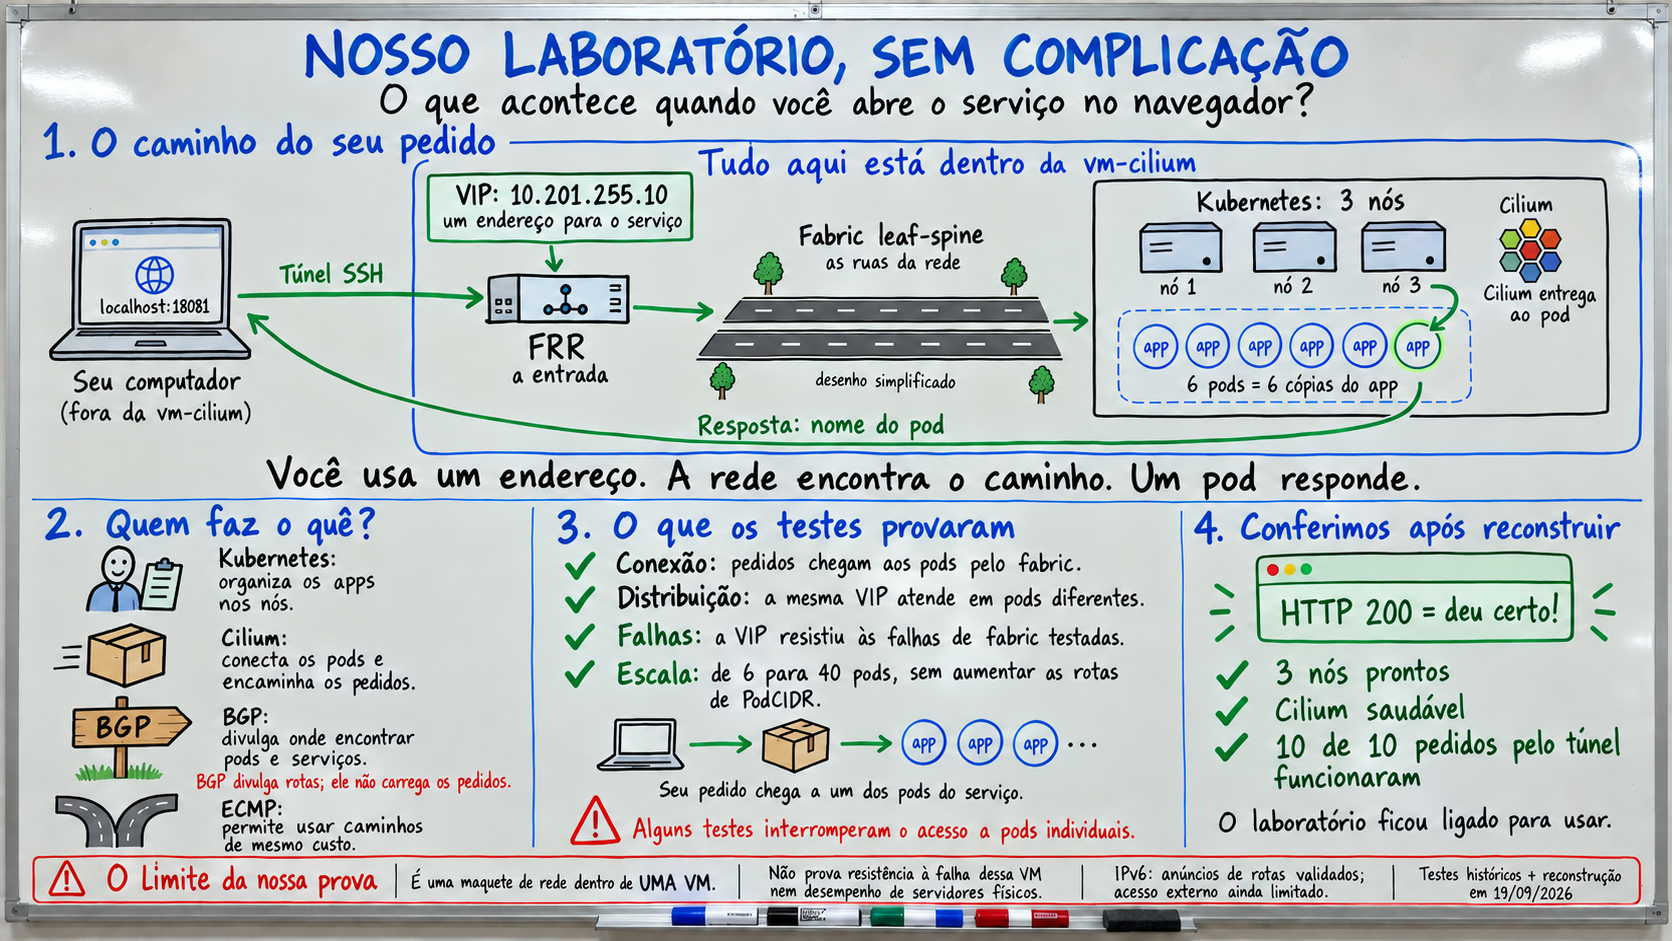
\includegraphics[width=\textwidth,height=0.72\textheight,keepaspectratio]{diagramas/06-laboratorio-explicado-iniciantes.png}
\fonte{elaborada pelo autor (2026).}
\end{figure}

Endereços que aparecem nos exercícios:

\begin{quadro}[!htbp]
\caption{Endereços usados nos exercícios}
\footnotesize
\begin{tabularx}{\textwidth}{|>{\raggedright\arraybackslash\hsize=1.013\hsize}X|>{\raggedright\arraybackslash\hsize=0.487\hsize}X|>{\raggedright\arraybackslash\hsize=1.500\hsize}X|}
\hline
\textbf{Recurso} & \textbf{Lab \texttt{k01}} & \textbf{Sandbox \texttt{p003-{}\allowbreak{}gw}} \\
\hline
PodCIDR IPv4 por nó & \texttt{10.\allowbreak{}244.\allowbreak{}x.\allowbreak{}0/\allowbreak{}24} & \texttt{10.\allowbreak{}245.\allowbreak{}x.\allowbreak{}0/\allowbreak{}24}
(IPAM \texttt{kubernetes}) \\
\hline
Pool de VIPs & \texttt{10.\allowbreak{}201.\allowbreak{}255.\allowbreak{}0/\allowbreak{}24},
VIP \texttt{10.\allowbreak{}201.\allowbreak{}255.\allowbreak{}10} & \texttt{10.\allowbreak{}202.\allowbreak{}255.\allowbreak{}0/\allowbreak{}24},
VIP \texttt{10.\allowbreak{}202.\allowbreak{}255.\allowbreak{}10} \\
\hline
Cliente externo ao cluster & \texttt{client-{}\allowbreak{}ext}
\texttt{203.\allowbreak{}0.\allowbreak{}113.\allowbreak{}10} & \texttt{fabric-{}\allowbreak{}client}
\texttt{198.\allowbreak{}19.\allowbreak{}0.\allowbreak{}10} \\
\hline
Gateway & não há & \texttt{p003-{}\allowbreak{}main} no namespace
\texttt{p003-{}\allowbreak{}gateway}, listeners 8080/HTTP, 15432/TCP,
15353/UDP \\
\hline
Rede do tenant OpenStack & não há & \texttt{10.\allowbreak{}30.\allowbreak{}0.\allowbreak{}0/\allowbreak{}24}
(subnet-a), externa
\texttt{10.\allowbreak{}40.\allowbreak{}0.\allowbreak{}0/\allowbreak{}24} \\
\hline
\end{tabularx}
\fonte{elaborado pelo autor (2026).}
\end{quadro}

\FloatBarrier

\section*{\texorpdfstring{A pergunta central: cada pod anuncia \texttt{/\allowbreak{}32}?}{A pergunta central: cada pod anuncia ?}}\label{a-pergunta-central-cada-pod-anuncia-32}
\addcontentsline{toc}{section}{A pergunta central: cada pod anuncia \texttt{/\allowbreak{}32}?}

\textbf{Não com o IPAM padrão.} Uma sessão BGP (Rekhter; Li; Hares, 2006) não é aberta
por pod. O agente Cilium em cada nó é o speaker e anuncia o \textbf{PodCIDR \texttt{/\allowbreak{}24} do
nó} (Cilium Authors, 2026b). Um pod com
\texttt{10.\allowbreak{}244.\allowbreak{}1.\allowbreak{}27} está coberto por \texttt{10.\allowbreak{}244.\allowbreak{}1.\allowbreak{}0/\allowbreak{}24}; não nasce sessão nem anúncio
para \texttt{10.\allowbreak{}244.\allowbreak{}1.\allowbreak{}27/\allowbreak{}32}.

O serviço tem outra regra. O \texttt{echo-{}\allowbreak{}anycast} recebe a VIP \texttt{10.\allowbreak{}201.\allowbreak{}255.\allowbreak{}10}, usa
\texttt{external\allowbreak{}Traffic\allowbreak{}Policy:\allowbreak{} Cluster} e os três nós anunciam a mesma
\texttt{10.\allowbreak{}201.\allowbreak{}255.\allowbreak{}10/\allowbreak{}32}; o fabric instala vários próximos saltos e faz ECMP. A rota
representa o serviço e seus pontos de entrada, não cada backend.

Existe uma terceira forma, medida no Módulo 10: com Multi-Pool IPAM e
\texttt{mask\allowbreak{}Size:\allowbreak{} 32}, cada pod recebe um bloco \texttt{/\allowbreak{}32} próprio e o Cilium anuncia esse
bloco. O speaker continua sendo o nó. O que muda é a granularidade, a
quantidade de rotas e o momento em que um bloco é alocado e retirado.

\chapter{Baseline e o que o Cilium anuncia}\label{baseline-e-o-que-o-cilium-anuncia}

Ambiente: lab \texttt{k01}. Origem: P001 (REQ-001 a REQ-007). A Figura 3 sintetiza o entregável do módulo.

\begin{figure}[!htbp]
\caption{Síntese visual do entregável do Módulo 1: Baseline BGP, 3 PodCIDRs /24,
VIP /32 e Native Routing sem VXLAN}
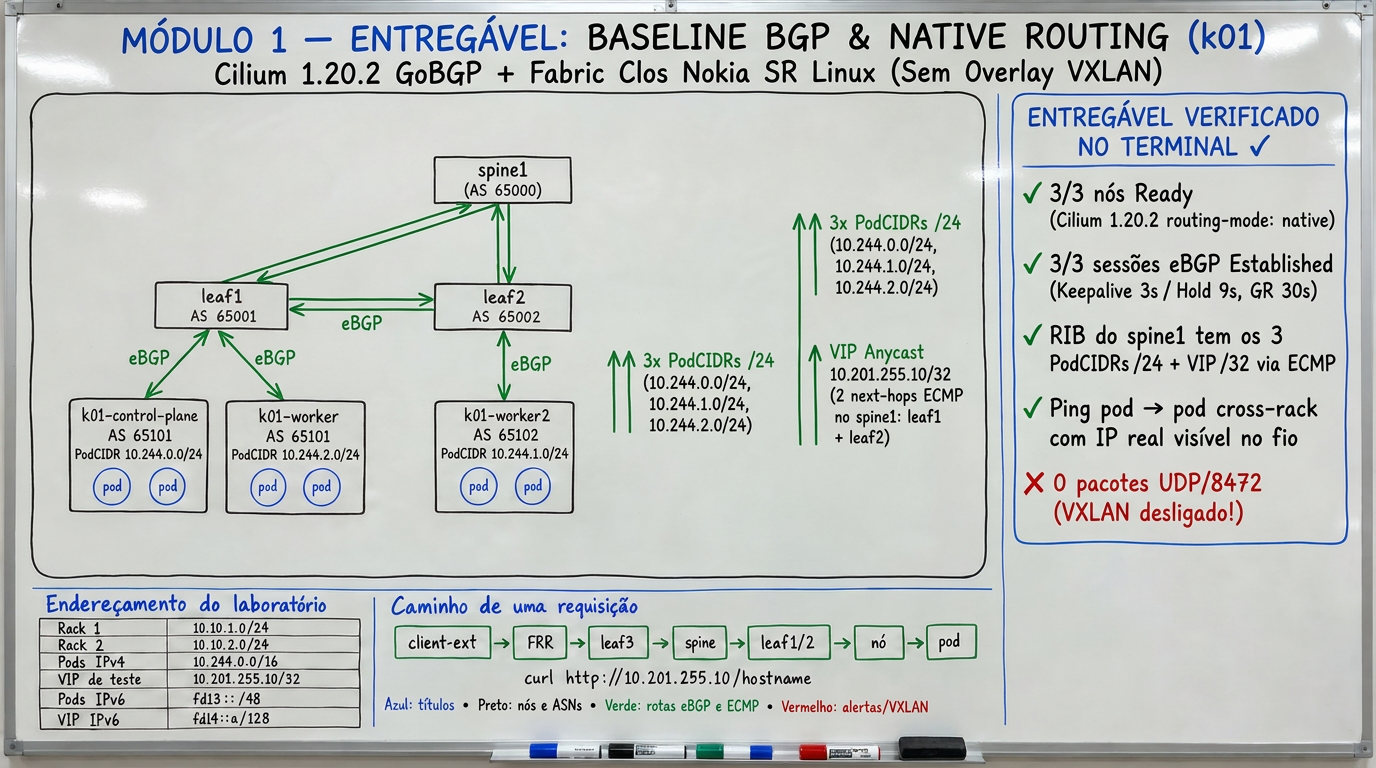
\includegraphics[width=\textwidth,height=0.72\textheight,keepaspectratio]{diagramas/m01-whiteboard-entregavel.png}
\fonte{elaborada pelo autor (2026).}
\end{figure}

\section{Conferir os containers}\label{conferir-os-containers}

Na \textbf{vm-cilium}:

\begin{verbatim}
sudo docker ps --format 'table {{.Names}}\t{{.Status}}' | grep -E 'clab-poc-k8s-kind|k01-'
$C1 ip -4 addr show dev eth1
\end{verbatim}

Esperado: \texttt{spine1}, \texttt{spine2}, \texttt{leaf1}, \texttt{leaf2}, \texttt{leaf3}, \texttt{border1},
\texttt{client-{}\allowbreak{}ext} e três \texttt{k01-{}\allowbreak{}*}; o \texttt{client-{}\allowbreak{}ext} mostra \texttt{203.\allowbreak{}0.\allowbreak{}113.\allowbreak{}10} uma vez. Esse
endereço pode sumir após um redeploy (lição L1 do RUNBOOK); sem ele todos os
probes do módulo falham sem falha real.

\section{Conferir o cluster e os PodCIDRs}\label{conferir-o-cluster-e-os-podcidrs}

\begin{verbatim}
k01 get nodes -o custom-columns=NODE:.metadata.name,PODCIDR:.spec.podCIDR,PODCIDRS:.spec.podCIDRs
k01 get pods -o wide
\end{verbatim}

Responda no caderno: qual \texttt{/\allowbreak{}24} cobre o IP de cada pod \texttt{echo-{}\allowbreak{}*}? A resposta
aponta para o bloco do nó, nunca para um \texttt{/\allowbreak{}32} do pod.

\section{Sessões e anúncios BGP}\label{sessuxf5es-e-anuxfancios-bgp}

\begin{verbatim}
sudo KUBECONFIG="$K01_KUBECONFIG" cilium --context kind-k01 bgp peers
sudo KUBECONFIG="$K01_KUBECONFIG" cilium --context kind-k01 bgp routes advertised ipv4 unicast
k01 get ciliumbgpclusterconfigs,ciliumbgppeerconfigs,ciliumbgpadvertisements
\end{verbatim}

Esperado: três sessões \texttt{established} (uma por nó, nunca uma por pod), timers
hold 9 s e keepalive 3 s, Graceful Restart habilitado com \texttt{restart\allowbreak{}Time} 30 s.
Entre os anúncios aparecem o PodCIDR do nó e a VIP \texttt{10.\allowbreak{}201.\allowbreak{}255.\allowbreak{}10/\allowbreak{}32}.

O anúncio da VIP só existe porque o \texttt{Cilium\allowbreak{}BGPAdvertisement} (Cilium Authors, 2026a)
tem um \texttt{selector}
com \texttt{bgp-{}\allowbreak{}advertise=\allowbreak{}true} e o Service carrega esse label. Sem o selector o
agente não anuncia nada de Service; este foi um achado repetido em nós reais.

\section{A rota no spine e a ausência de encapsulamento}\label{a-rota-no-spine-e-a-ausuxeancia-de-encapsulamento}

\begin{verbatim}
sudo docker exec clab-poc-k8s-kind-spine1 sr_cli \
  "show network-instance default route-table ipv4-unicast prefix 10.244.0.0/16 longer"
sudo docker exec clab-poc-k8s-kind-spine1 sr_cli \
  "show network-instance default route-table ipv4-unicast prefix 10.201.255.10/32 detail"
\end{verbatim}

Esperado: os três \texttt{/\allowbreak{}24} e a VIP com dois próximos saltos. Em native routing (Cilium Authors, 2026f)
o fabric vê o IP real do pod; a evidência histórica registra zero pacotes
UDP/8472 no fio e um handshake \texttt{203.\allowbreak{}0.\allowbreak{}113.\allowbreak{}10 \textgreater{} 10.\allowbreak{}244.\allowbreak{}2.\allowbreak{}198:\allowbreak{}8080} direto ao
pod.

\begin{quadro}[!htbp]
\caption{Registro do Módulo 1: valores esperados e observados}
\footnotesize
\begin{tabularx}{\textwidth}{|>{\raggedright\arraybackslash\hsize=1.292\hsize}X|>{\raggedright\arraybackslash\hsize=0.932\hsize}X|>{\raggedright\arraybackslash\hsize=0.775\hsize}X|}
\hline
\textbf{Item} & \textbf{Esperado} & \textbf{Observado} \\
\hline
Nós \texttt{Ready} & 3 &  \\
\hline
Sessões BGP & 3 established &  \\
\hline
PodCIDRs no spine & 3 &  \\
\hline
Next-hops da VIP no spine & 2 &  \\
\hline
\end{tabularx}
\fonte{elaborado pelo autor (2026).}
\end{quadro}

\chapter{VIP anycast e caminho do tráfego}\label{vip-anycast-e-caminho-do-truxe1fego}

Ambiente: lab \texttt{k01}. Origem: P001 (REQ-008 a REQ-010). A Figura 4 sintetiza o entregável do módulo.

\begin{figure}[!htbp]
\caption{Síntese visual do entregável do Módulo 2: VIP Anycast ECMP + Maglev,
ETP=Cluster vs ETP=Local e túnel SSH}
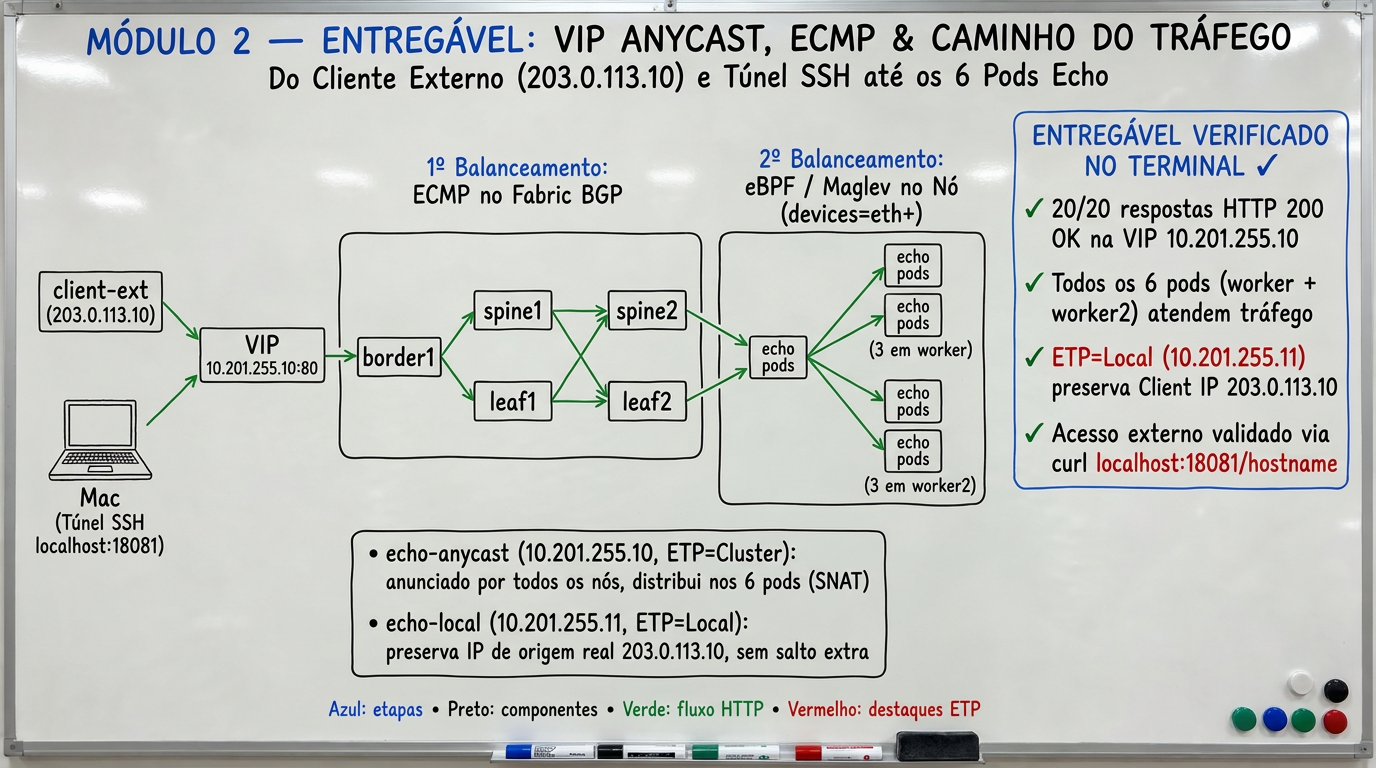
\includegraphics[width=\textwidth,height=0.72\textheight,keepaspectratio]{diagramas/m02-whiteboard-entregavel.png}
\fonte{elaborada pelo autor (2026).}
\end{figure}

\section{Requisições a partir do client-ext}\label{requisiuxe7uxf5es-a-partir-do-client-ext}

\begin{verbatim}
k01 get svc echo-anycast echo-local -o wide
for i in $(seq 1 20); do
  $C1 curl -fsS --max-time 5 http://10.201.255.10/hostname; echo
done | sort | uniq -c
\end{verbatim}

Esperado: \texttt{echo-{}\allowbreak{}anycast} com \texttt{10.\allowbreak{}201.\allowbreak{}255.\allowbreak{}10} e \texttt{external\allowbreak{}Traffic\allowbreak{}Policy:\allowbreak{} Cluster}; \texttt{echo-{}\allowbreak{}local} com \texttt{10.\allowbreak{}201.\allowbreak{}255.\allowbreak{}11} e \texttt{Local}. Vinte amostras não
garantem que todos os seis backends apareçam: ECMP e Maglev (Eisenbud et al., 2016) usam hashing. A
execução de referência registrou 20/20 HTTP 200 e seis pods distintos.

ICMP para a VIP não é respondido: o balanceador BPF atende TCP; \texttt{ping} na VIP
não é sinal de falha.

\section{O túnel para o Mac}\label{o-tuxfanel-para-o-mac}

No \textbf{Mac}:

\begin{verbatim}
export VM_CILIUM_HOST="${VM_CILIUM_HOST:-IP_DA_VM}"
curl --silent --fail --max-time 2 http://127.0.0.1:18081/hostname || \
ssh -i ~/.ssh/id_rsa -o IdentityAgent=SSH_AUTH_SOCK -o ExitOnForwardFailure=yes -N \
  -L 127.0.0.1:18081:10.201.255.10:80 ubuntu@"${VM_CILIUM_HOST}"
\end{verbatim}

O túnel termina no host da VM e encaminha uma porta local para a VIP. Ele não
publica a VIP na Internet. A rota do host que permite ao próprio host alcançar
a VIP é criada pelo instrutor com \texttt{scripts/\allowbreak{}06-{}\allowbreak{}expor-{}\allowbreak{}vip-{}\allowbreak{}na-{}\allowbreak{}vpc.\allowbreak{}sh}.

\section{O caminho e o fix que o tornou possível}\label{o-caminho-e-o-fix-que-o-tornou-possuxedvel}

\begin{verbatim}
Mac → túnel SSH → vm-cilium → clab-ext → border1/FRR → leaf3
    → spine → leaf do rack → nó Kubernetes → Cilium bpf-lb → Service → pod
\end{verbatim}

O balanceador BPF precisa estar anexado à interface do fabric (\texttt{eth1} no nó
kind). O controlador de devices do Cilium 1.20.1 pula veths sem rota default,
então o kit fixa \texttt{devices=\allowbreak{}eth+} nos values. Sem isso a VIP era roteada de volta
ao fabric em loop. Um \texttt{helm upgrade} que regenere o ConfigMap remove a chave;
o apêndice do instrutor mostra a verificação condicional.

Quando o cliente está fora da VM, na mesma VPC, o caminho é assimétrico: a
requisição entra pelo fabric e a resposta volta pela bridge docker do host,
porque o nó kind roteia a VPC por \texttt{eth0}. É uma propriedade da topologia, não
uma falha.

\chapter{Dual-stack IPv6 no plano de controle}\label{dual-stack-ipv6-no-plano-de-controle}

Ambiente: lab \texttt{k01} reconstruído com \texttt{values-{}\allowbreak{}dualstack.\allowbreak{}yaml}. Origem: P002-S001. A Figura 5 sintetiza o entregável do módulo.

\begin{figure}[!htbp]
\caption{Síntese visual do entregável do Módulo 3: Dual-Stack IPv6 no plano de
controle BGP e fronteira do underlay L3}
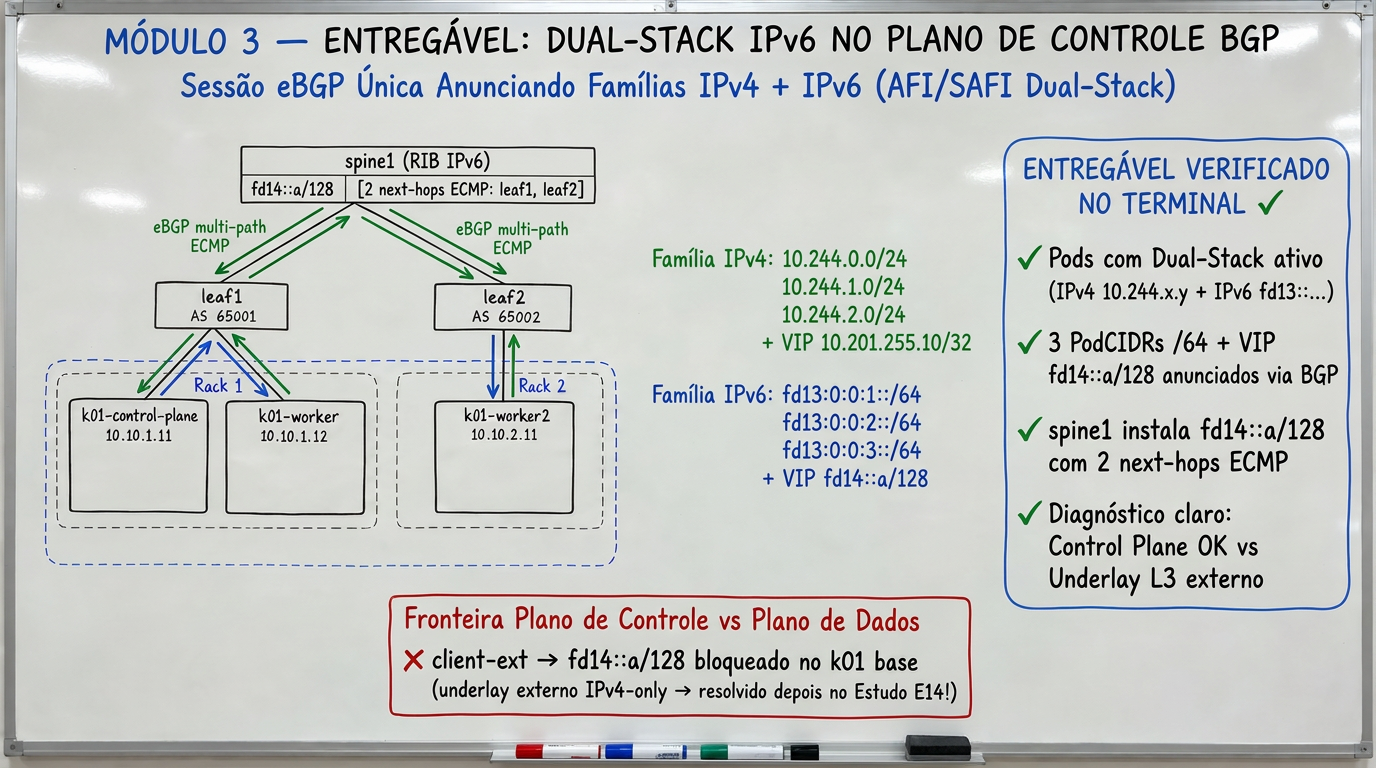
\includegraphics[width=\textwidth,height=0.72\textheight,keepaspectratio]{diagramas/m03-whiteboard-entregavel.png}
\fonte{elaborada pelo autor (2026).}
\end{figure}

\section{Ler o que foi provado}\label{ler-o-que-foi-provado}

\begin{verbatim}
k01 get nodes -o custom-columns=NODE:.metadata.name,PODCIDRS:.spec.podCIDRs
sudo KUBECONFIG="$K01_KUBECONFIG" cilium --context kind-k01 bgp routes advertised ipv6 unicast
sudo docker exec clab-poc-k8s-kind-spine1 sr_cli \
  "show network-instance default route-table ipv6-unicast prefix fd14::a/128 detail"
\end{verbatim}

Esperado: cada nó com dois PodCIDRs (\texttt{10.\allowbreak{}244.\allowbreak{}x.\allowbreak{}0/\allowbreak{}24} e \texttt{fd13:\allowbreak{}0:\allowbreak{}0:\allowbreak{}x:\allowbreak{}:\allowbreak{}/\allowbreak{}64}), os
três \texttt{/\allowbreak{}64} no spine e a VIP \texttt{fd14:\allowbreak{}:\allowbreak{}a/\allowbreak{}128} com dois próximos saltos. Uma única
sessão BGP transporta as duas famílias; a convergência do plano de controle
vale para ambas.

\section{O que a topologia não entrega}\label{o-que-a-topologia-nuxe3o-entrega}

A VIP IPv6 não é alcançável do \texttt{client-{}\allowbreak{}ext}: o underlay externo do lab é
IPv4-only e next-hops IPv4-mapped não encaminham IPv6. O tráfego pod→pod IPv6
cross-node flui pela rede kind, não pelo fabric. São limites do lab em
containers, não do Cilium nem do SR Linux. Não apresente alcance IPv6 fim a fim
como demonstrado.

Quatro configurações são obrigatórias e ficaram no kit: \texttt{ipv6.\allowbreak{}enabled:\allowbreak{} true}
nos values, \texttt{ip\allowbreak{}Family:\allowbreak{} dual} com dois \texttt{pod\allowbreak{}Subnet} no kind, \texttt{afi-{}\allowbreak{}safi ipv6-{}\allowbreak{}unicast} nos grupos \texttt{rack*-{}\allowbreak{}k8s} dos leaves e \texttt{multipath ipv6-{}\allowbreak{}unicast} nos
spines.

\chapter{Falhas, Graceful Restart e convergência}\label{falhas-graceful-restart-e-converguxeancia}

Ambiente: lab \texttt{k01}. Origem: P001 REQ-011, P002-S002 e P002-S004. Os gatilhos
de falha são tarefa do instrutor; a pessoa estudante lê e interpreta. A Figura 6 sintetiza o entregável do módulo.

\begin{figure}[!htbp]
\caption{Síntese visual do entregável do Módulo 4: Resiliência a falhas de
fabric, BGP Graceful Restart e convergência ECMP}
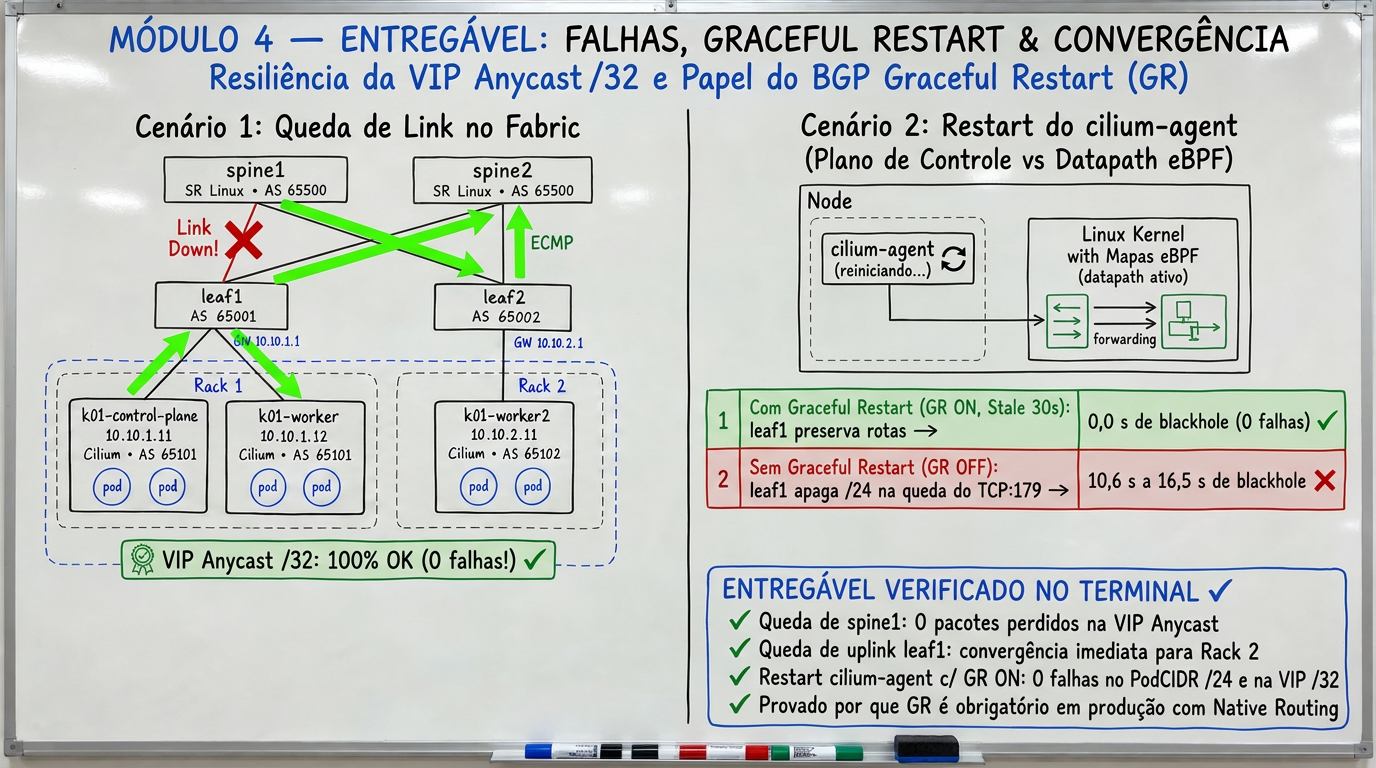
\includegraphics[width=\textwidth,height=0.72\textheight,keepaspectratio]{diagramas/m04-whiteboard-entregavel.png}
\fonte{elaborada pelo autor (2026).}
\end{figure}

\section{Como se mede um blackhole}\label{como-se-mede-um-blackhole}

Três loops de \texttt{curl} com timeout de 2 s rodam no \texttt{client-{}\allowbreak{}ext} contra a VIP
anycast, um pod do rack 1 (caminho único) e um pod do rack 2. Blackhole real é
o \textbf{maior intervalo sem nenhum OK}; timeouts encadeados não contam (lição L4).
Falhas de SR Linux são provocadas com \texttt{admin-{}\allowbreak{}state disable} via \texttt{sr\_\allowbreak{}cli},
nunca com \texttt{docker stop}, que destrói a wiring veth (lição L2).

\section{Resultados medidos}\label{resultados-medidos}

\begin{table}[!htbp]
\caption{Efeito das falhas de fabric e de agente sobre a VIP anycast e o PodCIDR}
\footnotesize
\begin{tabularx}{\textwidth}{>{\raggedright\arraybackslash\hsize=0.942\hsize}X>{\raggedright\arraybackslash\hsize=1.008\hsize}X>{\raggedright\arraybackslash\hsize=1.149\hsize}X>{\raggedright\arraybackslash\hsize=0.901\hsize}X}
\toprule
\textbf{Falha} & \textbf{VIP anycast} & \textbf{PodCIDR do rack afetado} & \textbf{Reconvergência} \\
\midrule
Restart do agent, GR ON & 0 falhas & sem blackhole & datapath BPF pinado sobrevive \\
Restart do agent, GR OFF & 0 falhas (outros nós anunciam) & blackhole 10,6 s (P001) a 16,5 s (P002) & até o novo agent reanunciar \\
Drain do nó & blip de 50 a 300 ms no início da evicção & pods evictados & GR irrelevante: a sessão não cai \\
1 spine de 2 & 100\% OK em 28,7 mil amostras & n/a & BGP re-up 33 a 38 s \\
1 leaf & 100\% OK (anycast segue pelo outro rack) & blackhole total do rack por 107 a 138 s & dados +44 a 48 s após enable \\
Spine 2 + leaf 1 juntos & 100\% OK em 34 mil amostras & blackhole total do rack 1 & lab sobrevive degradado \\
Flap simultâneo de 2 workers, GR ON & 0 de 19451 falhas & 2,4\% a 4,4\% de falhas, maxgap 2 a 4 s, sem blackhole & agents \textasciitilde52 s, estável \textasciitilde82 s \\
\bottomrule
\end{tabularx}
\fonte{elaborada pelo autor com dados de P001 (REQ-011), P002-S002 e P002-S004
(2026).}
\end{table}

Leituras que a pessoa estudante deve conseguir explicar:

\begin{itemize}
\tightlist
\item
  a VIP anycast \texttt{/\allowbreak{}32} com ECMP foi imune a todas as falhas de fabric testadas;
\item
  o PodCIDR é caminho único por rack quando o nó é single-homed; a falha do leaf isola o rack;
\item
  Graceful Restart elimina o blackhole de PodCIDR no restart do agent, em um nó ou em vários;
\item
  dual-homing do nó daria ECMP ao PodCIDR; o simulador SR Linux não estabelece TCP/179 em porta adicionada em runtime, então isso fica para um cluster real.
\end{itemize}

\section{O que a API do Cilium não expõe}\label{o-que-a-api-do-cilium-nuxe3o-expuxf5e}

\texttt{Cilium\allowbreak{}BGPPeer\allowbreak{}Config} v2 na versão 1.20.x tem \texttt{timers}, \texttt{graceful\allowbreak{}Restart},
\texttt{ebgp\allowbreak{}Multihop}, \texttt{families} e \texttt{auth\allowbreak{}Secret\allowbreak{}Ref}. Não há campo BFD (Katz; Ward, 2010). A detecção de
falha de sessão hoje é hold 9 s e keepalive 3 s, o menor valor aceito na
validação do lab. Essa lacuna é o ponto de partida de um dos próximos estudos.

\chapter{Escala e desempenho}\label{escala-e-desempenho}

Ambiente: lab \texttt{k01}. Origem: P002-S003. A Figura 7 sintetiza o entregável do módulo.

\begin{figure}[!htbp]
\caption{Síntese visual do entregável do Módulo 5: Escala 6 a 40 pods sem crescer
a RIB, burst de +30 VIPs e throughput Native vs VXLAN}
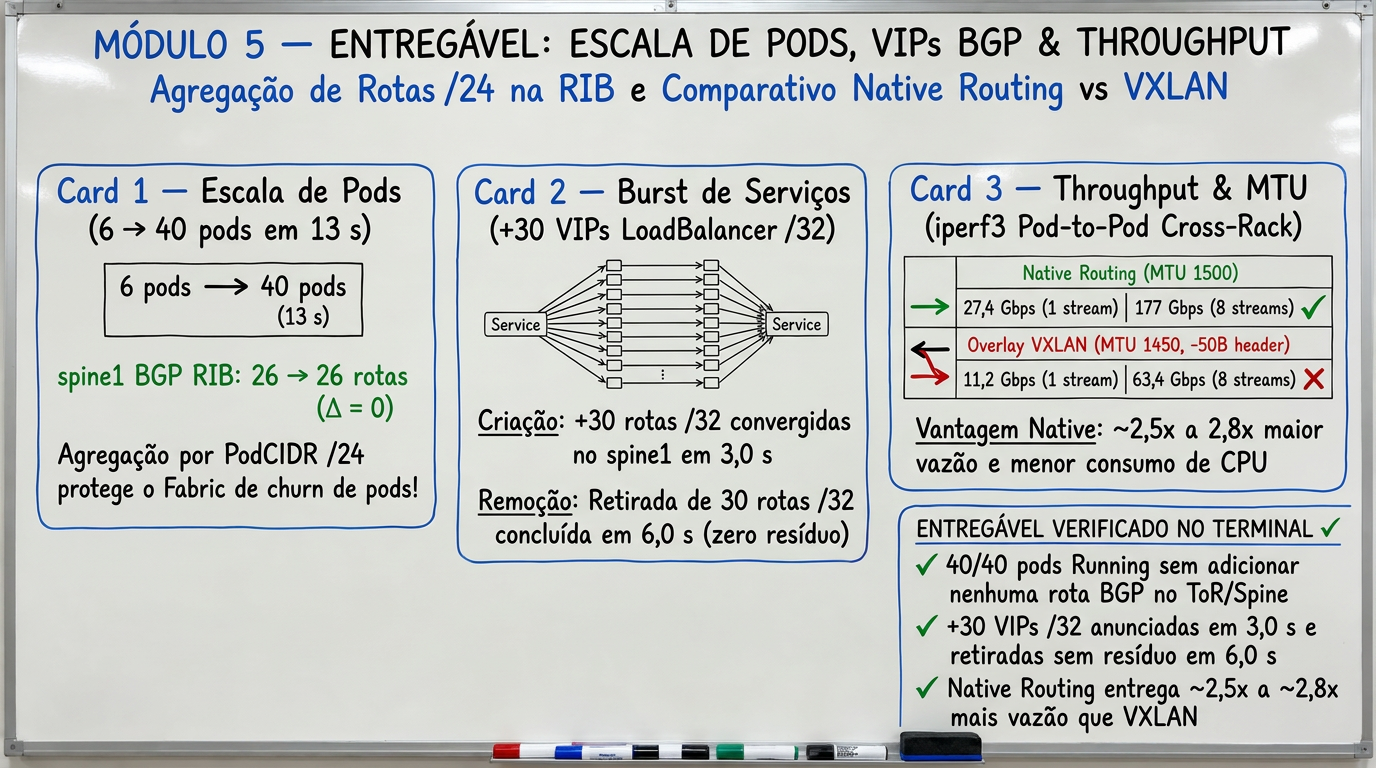
\includegraphics[width=\textwidth,height=0.72\textheight,keepaspectratio]{diagramas/m05-whiteboard-entregavel.png}
\fonte{elaborada pelo autor (2026).}
\end{figure}

\section{O que a pessoa estudante confere}\label{o-que-a-pessoa-estudante-confere}

\begin{verbatim}
sudo docker exec clab-poc-k8s-kind-spine1 sr_cli \
  "show network-instance default route-table ipv4-unicast summary"
k01 get deploy echo
\end{verbatim}

Anote o total de rotas IPv4 no spine e o número de réplicas. O instrutor pode
escalar o \texttt{echo} de 6 para 40 réplicas; repita o primeiro comando e compare.

\section{Resultados medidos}\label{resultados-medidos-1}

\begin{table}[!htbp]
\caption{Resultados de escala e desempenho no lab \texttt{k01}}
\footnotesize
\begin{tabularx}{\textwidth}{>{\raggedright\arraybackslash\hsize=0.773\hsize}X>{\raggedright\arraybackslash\hsize=1.227\hsize}X}
\toprule
\textbf{Eixo} & \textbf{Resultado} \\
\midrule
Pods 6 → 40 & 13 s até Ready; RIB do fabric inalterado (26 = 26): o
\texttt{/\allowbreak{}24} agrega \\
+10 VIPs \texttt{/\allowbreak{}32} & primeira no spine em 1,3 s; 10/10 em 4,2 s; ECMP de 2 next-hops por VIP \\
Burst de +30 VIPs & 30/30 em 3,0 s; withdrawal completo em 6,0 s \\
Throughput pod→pod cross-node & 27,5 Gb/s com 1 fluxo; 177 Gb/s com 8 fluxos; 193 Gb/s no sentido
reverso \\
Latência pod→pod & 0,094 ms ocioso; 0,039 ms sob 177 Gb/s, 0\% perda \\
VIP sob carga & 0 falhas em \textasciitilde24,7 mil requisições \\
Overlay VXLAN versus native & MTU 1450 versus 1500; 11,2 versus 27,4 Gb/s com 1 fluxo \\
\bottomrule
\end{tabularx}
\fonte{elaborada pelo autor com dados de P002-S003 (2026).}
\end{table}

A propriedade de escala é a agregação: pods escalam sem tocar no BGP e a RIB
cresce apenas com VIPs vezes nós, de forma linear. Os números absolutos vêm de
SR Linux em container e veths do kind; use apenas as relações.

\chapter{Gateway API HTTP, TCP e UDP por VIP BGP}\label{gateway-api-http-tcp-e-udp-por-vip-bgp}

Ambiente: sandbox \texttt{p003-{}\allowbreak{}gw}. Origem: P003-S003 e P003-S004. A implementação
da Gateway API pelo Cilium segue a documentação do projeto (Cilium Authors, 2026c). A Figura 8 sintetiza o entregável do módulo.

\begin{figure}[!htbp]
\caption{Síntese visual do entregável do Módulo 6: Gateway API HTTP, TCP e UDP
sobre a VIP BGP 10.202.255.10/32}
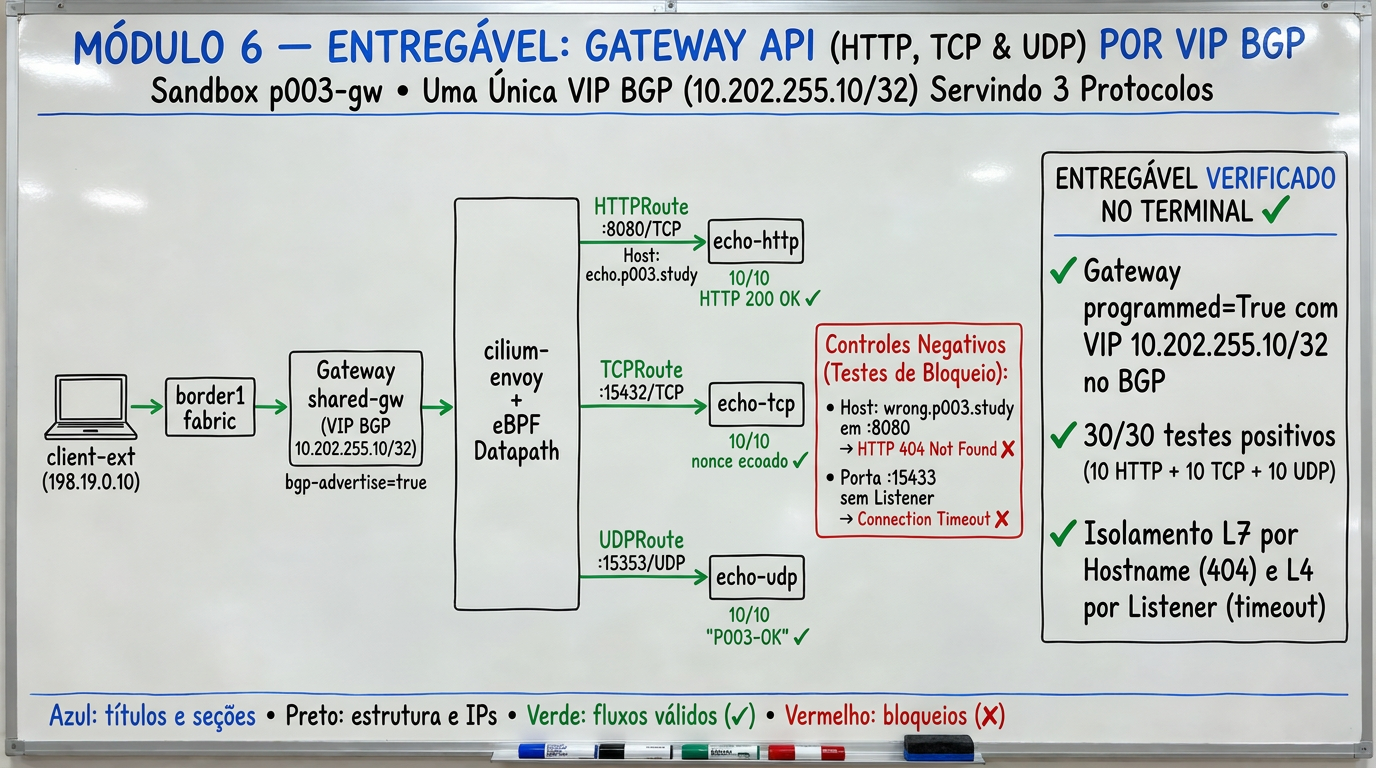
\includegraphics[width=\textwidth,height=0.72\textheight,keepaspectratio]{diagramas/m06-whiteboard-entregavel.png}
\fonte{elaborada pelo autor (2026).}
\end{figure}

\section{O Gateway e seu Service}\label{o-gateway-e-seu-service}

\begin{verbatim}
ks -n p003-gateway get gateway p003-main -o wide
ks -n p003-gateway get httproutes,tcproutes,udproutes
ks -n p003-gateway get svc -l bgp-advertise=true
sudo KUBECONFIG="$STUDY_KUBECONFIG" cilium --context kind-p003-gw \
  bgp routes advertised ipv4 unicast
\end{verbatim}

Esperado: Gateway \texttt{Programmed=\allowbreak{}True} com \texttt{IPAddress 10.\allowbreak{}202.\allowbreak{}255.\allowbreak{}10}; o Service
gerado pelo Cilium com \texttt{EXTERNAL-{}\allowbreak{}IP 10.\allowbreak{}202.\allowbreak{}255.\allowbreak{}10} e o label
\texttt{bgp-{}\allowbreak{}advertise=\allowbreak{}true}, que vem de \texttt{spec.\allowbreak{}infrastructure.\allowbreak{}labels} do Gateway, não
de \texttt{metadata.\allowbreak{}labels}. A VIP aparece nos anúncios BGP dos três nós.

\section{Um listener por protocolo, com controle negativo}\label{um-listener-por-protocolo-com-controle-negativo}

\begin{verbatim}
VIP=10.202.255.10
$C2 curl -sS --retry 0 --max-time 5 -H 'Host: echo.p003.study' \
  -w '\n%{http_code}\n' "http://$VIP:8080/hostname"
$C2 curl -sS --retry 0 --max-time 5 -H 'Host: wrong.example' \
  -o /dev/null -w '%{http_code}\n' "http://$VIP:8080/hostname"
$C2 sh -c "echo P003-nonce-1 | nc -w 3 $VIP 15432"
$C2 dig @"$VIP" -p 15353 study.p003 TXT +short +notcp +tries=1 +time=2
$C2 sh -c "echo P003-gw04 | nc -w 3 $VIP 15433"
\end{verbatim}

\begin{quadro}[!htbp]
\caption{Registro do Módulo 6: listeners e controle negativo}
\footnotesize
\begin{tabularx}{\textwidth}{|>{\raggedright\arraybackslash\hsize=1.034\hsize}X|>{\raggedright\arraybackslash\hsize=1.304\hsize}X|>{\raggedright\arraybackslash\hsize=0.661\hsize}X|}
\hline
\textbf{Caso} & \textbf{Esperado} & \textbf{Observado} \\
\hline
HTTP com Host correto & 200 e hostname de um pod
\texttt{http-{}\allowbreak{}echo-{}\allowbreak{}*} &  \\
\hline
HTTP com Host errado & 404 do Envoy &  \\
\hline
TCP 15432 & o nonce volta idêntico &  \\
\hline
UDP 15353 & \texttt{"P003-{}\allowbreak{}OK"} &  \\
\hline
TCP 15433 sem listener & timeout, nenhuma chegada na fixture &  \\
\hline
\end{tabularx}
\fonte{elaborado pelo autor (2026).}
\end{quadro}

A matriz de referência registrou 30/30 em cada listener, 503 com
EndpointSlice vazio quando o backend foi escalado a zero e recuperação
completa ao restaurar. Quando o instrutor troca o \texttt{Cilium\allowbreak{}BGPAdvertisement}
por um selector que não casa, a \texttt{/\allowbreak{}32} some do spine em cerca de 15 s, a VIP
para de responder e o IP direto do pod continua funcionando: é o controle que
separa ``anúncio'' de ``serviço''.

\section{\texorpdfstring{Achado: \texttt{host\allowbreak{}Network} do Gateway não expõe listener no nó}{Achado:  do Gateway não expõe listener no nó}}\label{achado-hostnetwork-do-gateway-nuxe3o-expuxf5e-listener-no-nuxf3}

\texttt{gateway\allowbreak{}API.\allowbreak{}host\allowbreak{}Network.\allowbreak{}enabled} no Cilium 1.20.2 é uma feature dos listeners
Envoy (L7), controlada por \texttt{nodes.\allowbreak{}match\allowbreak{}Labels}. Com o seletor vazio, nenhum
socket abre no IP do nó nas portas 8080, 15432 ou 15353. Os probes ao nó
nessas portas deram 180/180 falhas; os \texttt{node\allowbreak{}Port} do Service gerado deram
180/180 sucessos. Para expor TCP/UDP no nó, o caminho suportado é o NodePort
ou a VIP por BGP.

\chapter{Autorização externa na borda}\label{autorizauxe7uxe3o-externa-na-borda}

Ambiente: sandbox \texttt{p003-{}\allowbreak{}gw}. Origem: P003-S005, P003-S006 e P003-S009 (T05).
O ExternalAuth do Gateway API é experimental na 1.20.2; o CRD \texttt{HTTPRoute}
recebeu o schema experimental por um patch de spec, porque o
\texttt{experimental-{}\allowbreak{}install.\allowbreak{}yaml} estoura o limite de annotations no Kubernetes
1.35.0. A Figura 9 sintetiza o entregável do módulo.

\begin{figure}[!htbp]
\caption{Síntese visual do entregável do Módulo 7: ExternalAuth HTTP e gRPC na
borda Envoy e garantia 100\% Fail-Closed}
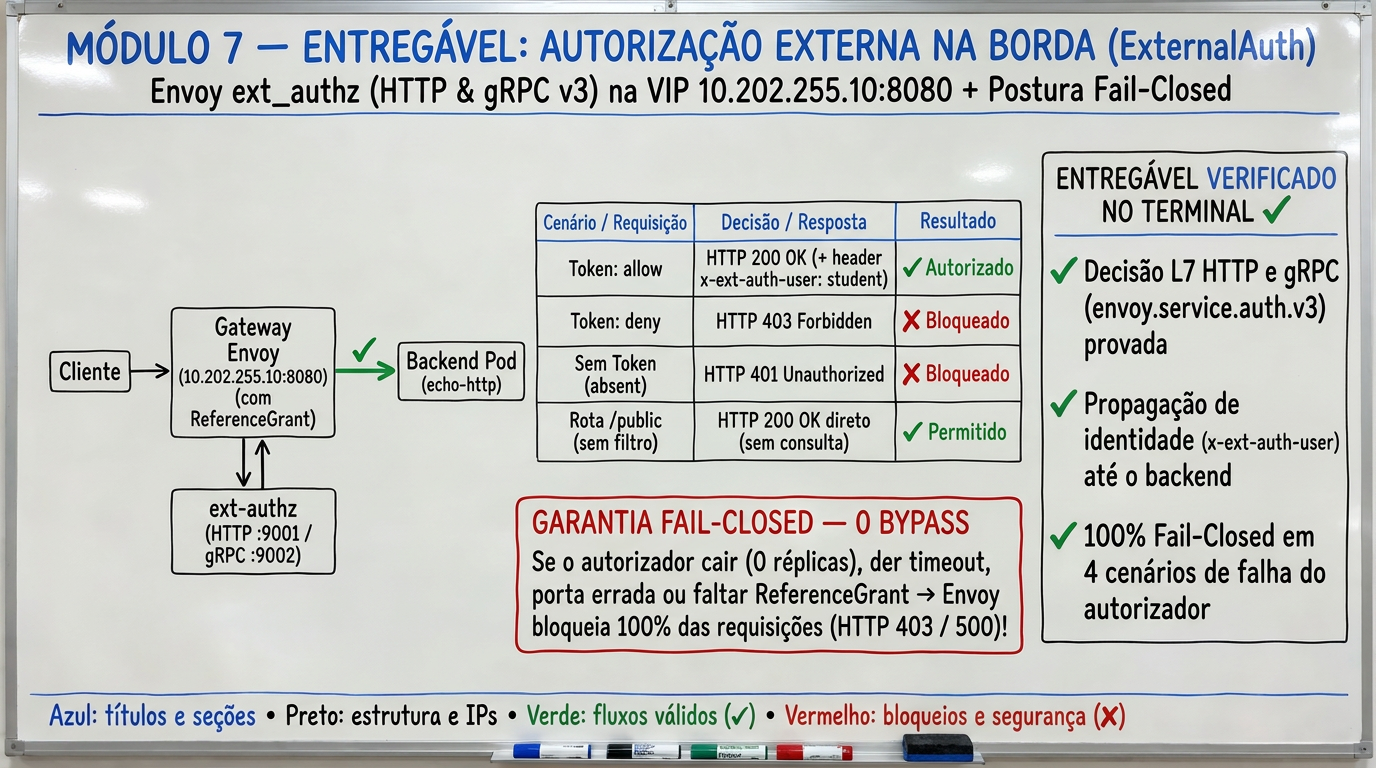
\includegraphics[width=\textwidth,height=0.72\textheight,keepaspectratio]{diagramas/m07-whiteboard-entregavel.png}
\fonte{elaborada pelo autor (2026).}
\end{figure}

\section{A fixture}\label{a-fixture}

Um serviço Go em \texttt{studies/\allowbreak{}p003/\allowbreak{}fixtures/\allowbreak{}auth/\allowbreak{}} decide \texttt{allow}, \texttt{deny} ou
\texttt{absent} a partir do header \texttt{X-{}\allowbreak{}Lab-{}\allowbreak{}Decision} e registra cada consulta com o
\texttt{X-{}\allowbreak{}Lab-{}\allowbreak{}Request-{}\allowbreak{}ID}. Ele fala HTTP e gRPC (\texttt{envoy.\allowbreak{}service.\allowbreak{}auth.\allowbreak{}v3}). Não é um
IdP; serve para observar a decisão, não para autenticar pessoas.

\section{Três decisões, dois protocolos}\label{truxeas-decisuxf5es-dois-protocolos}

\begin{verbatim}
for d in allow deny ""; do
  $C2 curl -sS --retry 0 --max-time 15 -H 'Host: echo.p003.study' \
    ${d:+-H "X-Lab-Decision: $d"} -H "X-Lab-Request-ID: aluno-$RANDOM" \
    -o /dev/null -w "decisao=${d:-absent} http=%{http_code}\n" \
    "http://10.202.255.10:8080/protected-http"
done
$C2 curl -sS --retry 0 -o /dev/null -w 'public http=%{http_code}\n' \
  -H 'Host: echo.p003.study' http://10.202.255.10:8080/public
\end{verbatim}

\begin{table}[!htbp]
\caption{Código HTTP por decisão do autorizador externo}
\footnotesize
\begin{tabularx}{\textwidth}{>{\raggedright\arraybackslash\hsize=1.602\hsize}X>{\raggedright\arraybackslash\hsize=0.699\hsize}X>{\raggedright\arraybackslash\hsize=0.699\hsize}X}
\toprule
\textbf{Decisão} & \textbf{HTTP} & \textbf{gRPC} \\
\midrule
allow & 200 & 200 \\
deny & 403 & 403 \\
absent & 401 & 401 \\
rota pública sem auth & 200 & 200 \\
\bottomrule
\end{tabularx}
\fonte{elaborada pelo autor com dados de P003-S005 e P003-S006, matriz A01--A10
(2026).}
\end{table}

A matriz A01--A10 executou 900 requisições com esse resultado. O header
forjado \texttt{X-{}\allowbreak{}Lab-{}\allowbreak{}User} enviado pelo cliente não aparece na resposta (A08). A
rota pública não consulta o autorizador (A09).

\section{Fail-closed sob degradação}\label{fail-closed-sob-degradauxe7uxe3o}

\begin{table}[!htbp]
\caption{Comportamento fail-closed do ExternalAuth sob degradação}
\footnotesize
\begin{tabularx}{\textwidth}{>{\raggedright\arraybackslash\hsize=1.069\hsize}X>{\raggedright\arraybackslash\hsize=0.872\hsize}X>{\raggedright\arraybackslash\hsize=0.872\hsize}X>{\raggedright\arraybackslash\hsize=1.187\hsize}X}
\toprule
\textbf{Cenário} & \textbf{HTTP} & \textbf{gRPC} & \textbf{Conclusão} \\
\midrule
autorizador escalado a zero & 403 em 2 ms & 403 & fail-closed \\
autorizador com atraso de 15 s & 403 após 10 s & 403 após \textasciitilde200 ms & timeout do Envoy difere por protocolo \\
\texttt{backend\allowbreak{}Ref} inexistente & 500 & 500 & \texttt{Resolved\allowbreak{}Refs=\allowbreak{}False} \\
porta errada & 403 & 403 & \texttt{Backend\allowbreak{}Not\allowbreak{}Found} \\
cross-namespace sem \texttt{Reference\allowbreak{}Grant} & 500 & 500 & \texttt{Ref\allowbreak{}Not\allowbreak{}Permitted} \\
\texttt{Reference\allowbreak{}Grant} removido durante probes & 403 → 500 em até 2 s & 200 → 500 em até 2 s & revogação sem bypass \\
\bottomrule
\end{tabularx}
\fonte{elaborada pelo autor com dados de P003-S005, P003-S006 e P003-S009
(2026).}
\end{table}

Nenhum cenário liberou a aplicação. Dois defeitos ficaram registrados na
1.20.2: com Grant válido, a rota HTTP cross-namespace com decisão allow pendura
(gRPC funciona), e um bloco \texttt{http:\allowbreak{} \{\}} vazio devolve 401 para todas as
decisões. \texttt{allowed\allowbreak{}Response\allowbreak{}Headers} não encaminhou os headers do autorizador ao
cliente.

\chapter{WireGuard em native routing e VXLAN}\label{wireguard-em-native-routing-e-vxlan}

Ambiente: sandbox \texttt{p003-{}\allowbreak{}gw}. Origem: P003-S007 e P003-S008. Os perfis são
trocados pelo instrutor com \texttt{helm upgrade}; a pessoa estudante confere
interfaces e capturas. O Cilium usa o WireGuard (Donenfeld, 2017) na interface
\texttt{cilium\_\allowbreak{}wg0}, na porta UDP 51871 (Cilium Authors, 2026i). A Figura 10 sintetiza o entregável do módulo.

\begin{figure}[!htbp]
\caption{Síntese visual do entregável do Módulo 8: WireGuard W0/W1/W2 em
UDP/51871 e fronteira de criptografia do hostns no Native Routing}
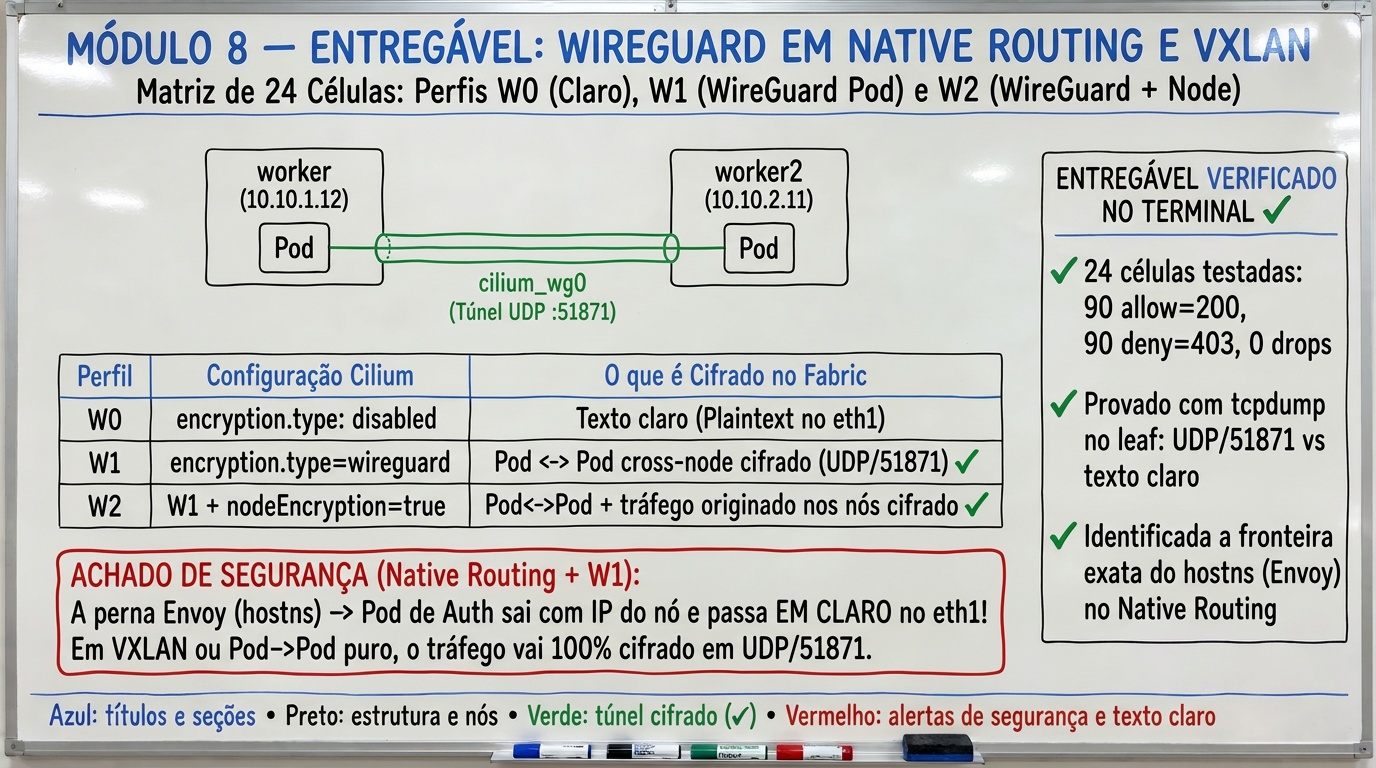
\includegraphics[width=\textwidth,height=0.72\textheight,keepaspectratio]{diagramas/m08-whiteboard-entregavel.png}
\fonte{elaborada pelo autor (2026).}
\end{figure}

\section{Três perfis}\label{truxeas-perfis}

\begin{quadro}[!htbp]
\caption{Perfis de criptografia W0, W1 e W2}
\footnotesize
\begin{tabularx}{\textwidth}{|>{\raggedright\arraybackslash\hsize=0.489\hsize}X|>{\raggedright\arraybackslash\hsize=0.937\hsize}X|>{\raggedright\arraybackslash\hsize=1.573\hsize}X|}
\hline
\textbf{Perfil} & \textbf{Configuração} & \textbf{Sinal na bridge do underlay} \\
\hline
W0 & criptografia desligada & native: payload em claro; VXLAN: UDP/8472 com payload em claro \\
\hline
W1 & \texttt{encryption.\allowbreak{}type=\allowbreak{}wireguard} & UDP/51871 para o tráfego pod→pod remoto \\
\hline
W2 & W1 +
\texttt{node\allowbreak{}Encryption.\allowbreak{}enabled=\allowbreak{}true} & UDP/51871 também para tráfego de nó \\
\hline
\end{tabularx}
\fonte{elaborado pelo autor (2026).}
\end{quadro}

\begin{verbatim}
ks -n kube-system exec ds/cilium -- cilium-dbg encrypt status
ks -n kube-system exec ds/cilium -- ip -br link show cilium_wg0
\end{verbatim}

\section{O que as 24 células mostraram}\label{o-que-as-24-cuxe9lulas-mostraram}

Quatro placements (auth e app no nó A ou no nó B, ingress fixo no nó A) vezes
três perfis vezes duas topologias (native e VXLAN): 90 allow com 200 e 90 deny
com 403 em cada célula, zero drops no \texttt{cilium-{}\allowbreak{}dbg monitor}. O handshake
Envoy→autorizador relatado na issue 46768 (Devantler, 2026) não se reproduziu na 1.20.2 em nenhuma
combinação.

O achado de segurança é outro: em native routing, a perna Envoy→pod de auth
por IP direto \textbf{atravessa em claro} no underlay mesmo com WireGuard de pod
ativo (20 IDs de requisição legíveis por célula com auth remoto). Em VXLAN a
mesma perna sai cifrada em W1 e W2. A exposição depende da topologia, não da
decisão de auth. Ao desenhar criptografia, trate o tráfego originado pelo
Envoy do nó como tráfego de nó.

\chapter{Tenants: rede, borda e configuração}\label{tenants-rede-borda-e-configurauxe7uxe3o}

Ambiente: sandbox \texttt{p003-{}\allowbreak{}gw}. Origem: P003-S009, matriz T01--T17. A Figura 11 sintetiza o entregável do módulo.

\begin{figure}[!htbp]
\caption{Síntese visual do entregável do Módulo 9: Isolamento Multi-Tenant
T01--T17 em 3 camadas (Rede CNP, Borda ExternalAuth/TLS e Governança
K8s)}
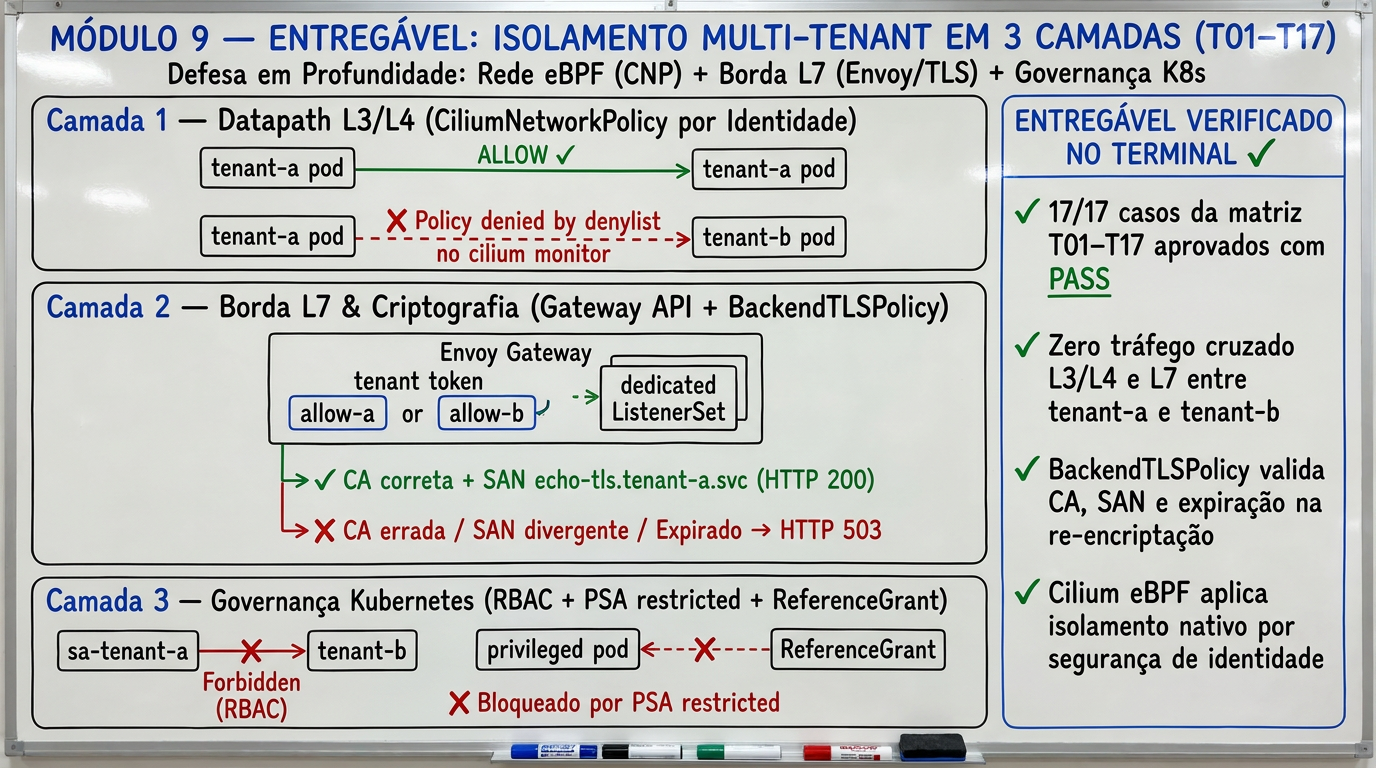
\includegraphics[width=\textwidth,height=0.72\textheight,keepaspectratio]{diagramas/m09-whiteboard-entregavel.png}
\fonte{elaborada pelo autor (2026).}
\end{figure}

\section{Três controles diferentes}\label{truxeas-controles-diferentes}

\begin{quadro}[!htbp]
\caption{Controles de isolamento de tenant}
\footnotesize
\begin{tabularx}{\textwidth}{|>{\raggedright\arraybackslash\hsize=0.588\hsize}X|>{\raggedright\arraybackslash\hsize=0.914\hsize}X|>{\raggedright\arraybackslash\hsize=1.499\hsize}X|}
\hline
\textbf{Controle} & \textbf{Mecanismo} & \textbf{O que impede} \\
\hline
Rede & \texttt{Cilium\allowbreak{}Network\allowbreak{}Policy} por identidade e
porta & A alcançar B e vice-versa em conexões novas \\
\hline
Borda & ExternalAuth no listener HTTP & usuário sem credencial na rota protegida \\
\hline
Configuração & RBAC + \texttt{allowed\allowbreak{}Routes} +
\texttt{allowed\allowbreak{}Listeners} +
\texttt{Reference\allowbreak{}Grant} + PSA \texttt{restricted} & tenant editar policy alheia, criar Gateway de contorno, subir pod
privilegiado \\
\hline
\end{tabularx}
\fonte{elaborado pelo autor (2026).}
\end{quadro}

\section{Ler um drop de policy}\label{ler-um-drop-de-policy}

\begin{verbatim}
ks get ciliumnetworkpolicies -A
ks -n kube-system exec ds/cilium -- \
  cilium-dbg monitor -t drop --related-to 0 2>/dev/null | head -20
\end{verbatim}

Com o instrutor gerando tráfego A→B, você deve ver drops com \texttt{Policy denied} e
o log da aplicação de destino vazio: o pacote não chega. Isso é diferente de
um 403 na borda, que é gerado pelo Envoy antes da aplicação.

\section{Resultados}\label{resultados}

Todos os 17 casos passaram. Os negativos foram reais: chamadas de API
impersonadas devolveram \texttt{Forbidden} (não apenas \texttt{can-{}\allowbreak{}i}), o PSA
\texttt{restricted:\allowbreak{}v1.\allowbreak{}35} rejeitou \texttt{host\allowbreak{}Network}, \texttt{privileged}, \texttt{host\allowbreak{}PID} e
\texttt{host\allowbreak{}Path}, e labels de tenant ausentes ou forjados não executaram. A TLS do
backend (\texttt{Backend\allowbreak{}TLSPolicy}) falhou antes do request HTTP com CA errada, SAN
errado ou certificado expirado.

Um detalhe que muda desenho: o ExternalAuth protege apenas o listener HTTP.
O listener TCP sob a mesma VIP respondeu 200 para o tenant errado até uma CNP
L4 ser aplicada (T07). Autorização L7 não é política L4.

\chapter{Multi-Pool IPAM: /24 versus /32}\label{multi-pool-ipam-24-versus-32}

Ambiente: sandbox \texttt{p003-{}\allowbreak{}gw}, com IPAM trocado para \texttt{multi-{}\allowbreak{}pool} pelo instrutor
e restaurado ao final. Origem: P003-S010, matriz I01--I10. A Figura 12 sintetiza o entregável do módulo.

\begin{figure}[!htbp]
\caption{Síntese visual do entregável do Módulo 10: Multi-Pool IPAM /24 vs /32,
BGP Communities e retenção preAllocate=8}
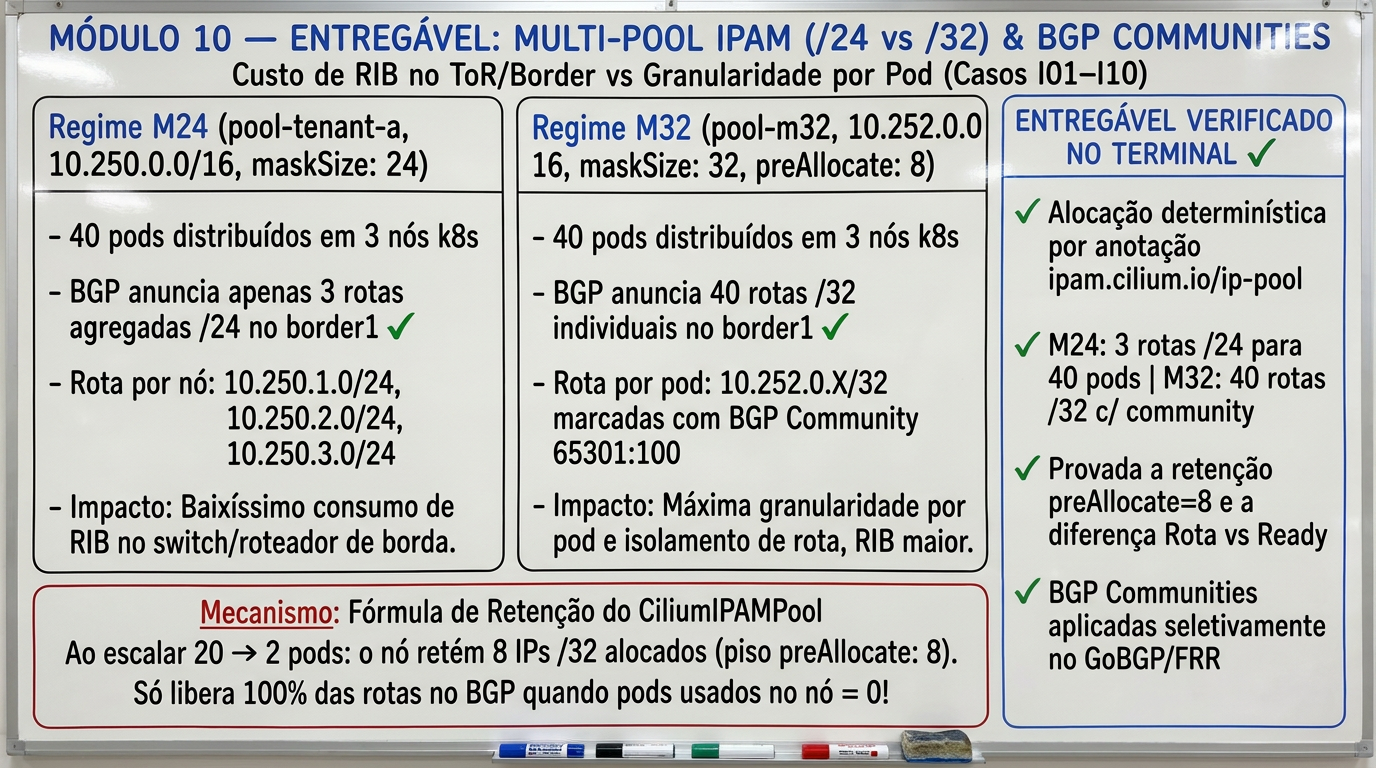
\includegraphics[width=\textwidth,height=0.72\textheight,keepaspectratio]{diagramas/m10-whiteboard-entregavel.png}
\fonte{elaborada pelo autor (2026).}
\end{figure}

\section{Dois braços com a mesma variável}\label{dois-brauxe7os-com-a-mesma-variuxe1vel}

\begin{quadro}[!htbp]
\caption{Braços M24 e M32 do estudo Multi-Pool IPAM}
\footnotesize
\begin{tabularx}{\textwidth}{|>{\raggedright\arraybackslash\hsize=0.923\hsize}X|>{\raggedright\arraybackslash\hsize=0.826\hsize}X|>{\raggedright\arraybackslash\hsize=0.826\hsize}X|>{\raggedright\arraybackslash\hsize=0.826\hsize}X|>{\raggedright\arraybackslash\hsize=1.599\hsize}X|}
\hline
\textbf{Braço} & \textbf{Pool} & \textbf{\texttt{mask\allowbreak{}Size}} & \textbf{\texttt{pre\allowbreak{}Allocate}} & \textbf{Anúncio} \\
\hline
M24 & \texttt{10.\allowbreak{}250.\allowbreak{}0.\allowbreak{}0/\allowbreak{}16} & 24 & 8 & \texttt{Cilium\allowbreak{}Pod\allowbreak{}IPPool} com community
\texttt{65301:\allowbreak{}100} \\
\hline
M32 & \texttt{10.\allowbreak{}252.\allowbreak{}0.\allowbreak{}0/\allowbreak{}16} & 32 & 8 & idem \\
\hline
\end{tabularx}
\fonte{elaborado pelo autor (2026).}
\end{quadro}

\begin{verbatim}
ks get ciliumpodippools -o wide
ks get ciliumnodes -o custom-columns=NODE:.metadata.name,POOLS:.spec.ipam.pools.allocated
sudo docker exec clab-p003-gw-fabric-border1 vtysh -c 'show ip bgp' | grep -E '10\.25[02]\.'
\end{verbatim}

\section{\texorpdfstring{O que muda entre \texttt{/\allowbreak{}24} e \texttt{/\allowbreak{}32}}{O que muda entre  e }}\label{o-que-muda-entre-24-e-32}

\begin{quadro}[!htbp]
\caption{Comportamento dos blocos \texttt{/\allowbreak{}24} e
\texttt{/\allowbreak{}32} no Multi-Pool IPAM}
\footnotesize
\begin{tabularx}{\textwidth}{|>{\raggedright\arraybackslash\hsize=0.727\hsize}X|>{\raggedright\arraybackslash\hsize=1.157\hsize}X|>{\raggedright\arraybackslash\hsize=1.116\hsize}X|}
\hline
\textbf{Pergunta} & \textbf{M24} & \textbf{M32} \\
\hline
Pod novo & cai num \texttt{/\allowbreak{}24} já alocado; zero eventos de bloco & cada pod ganha um \texttt{/\allowbreak{}32}; alocado e anunciado em 1 a
2 s \\
\hline
40 pods & 3 rotas no border & 40 rotas no border, uma por pod \\
\hline
Pod \texttt{Not\allowbreak{}Ready} sem delete & bloco e rota permanecem; IP direto responde 200; o Service exclui o pod & idêntico \\
\hline
Apagar 1 pod & bloco retido:
\texttt{round\allowbreak{}Up(\allowbreak{}in\allowbreak{}Use+8,\allowbreak{} 8)}
não encolhe & idêntico; o piso de \texttt{pre\allowbreak{}Allocate} domina \\
\hline
Voltar a zero pods & blocos \texttt{/\allowbreak{}24} retidos por mais de 120 s & encolhe em 42 s no operador e 48 s na RIB, até o piso de 8
\texttt{/\allowbreak{}32} por nó \\
\hline
Recriar pod no mesmo nó & IP novo dentro do mesmo \texttt{/\allowbreak{}24} & alterna entre \texttt{/\allowbreak{}32} recém-liberados; sem IP estável \\
\hline
Peer BGP do border desligado & prefixos somem em \textasciitilde10 s; pod e VIP dão 000 & idêntico \\
\hline
\end{tabularx}
\fonte{elaborado pelo autor com dados de P003-S010, matriz I01--I10 (2026).}
\end{quadro}

Duas lições. O datapath não gateia readiness: rota e alcance direto ao pod
existem enquanto o IP existir, e só o Service respeita \texttt{Ready}. A retirada de
um bloco depende de \texttt{pre\allowbreak{}Allocate}, não da morte do pod; um \texttt{/\allowbreak{}32} não é
``retirado quando o pod morre''.

\chapter{Tenant híbrido: pods e VMs OpenStack}\label{tenant-huxedbrido-pods-e-vms-openstack}

Ambiente: sandbox \texttt{p003-{}\allowbreak{}gw} + testbed OpenStack + VM em KVM real. Origem:
P003-S011 a S016. As sínteses públicas completas estão em
E08 e C5. A Figura 13 sintetiza o entregável do módulo.

\begin{figure}[!htbp]
\caption{Síntese visual do entregável do Módulo 11: Tenant híbrido Pod K8s ↔ VM
KVM/OpenStack e contraste Identidade (fromEndpoints) vs IP (fromCIDR)}
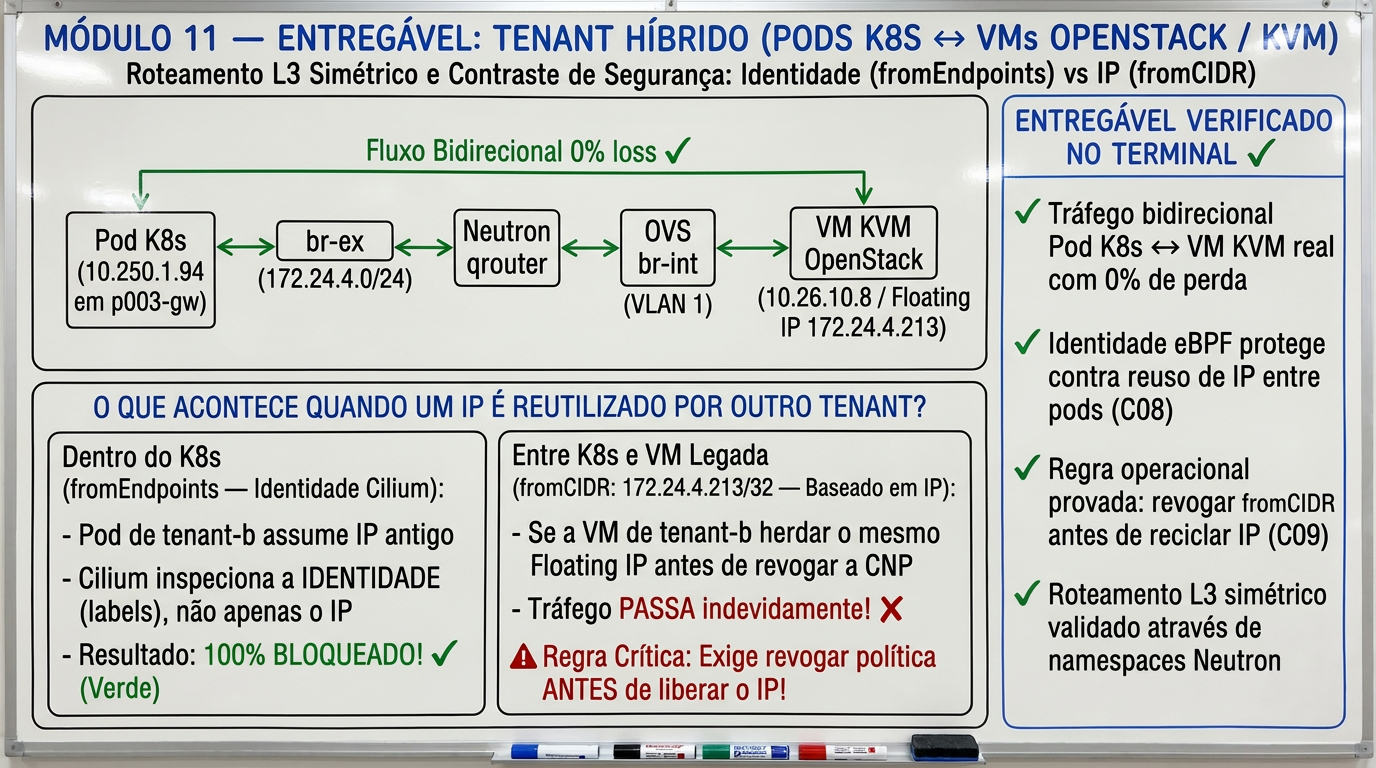
\includegraphics[width=\textwidth,height=0.72\textheight,keepaspectratio]{diagramas/m11-whiteboard-entregavel.png}
\fonte{elaborada pelo autor (2026).}
\end{figure}

\section{A pergunta}\label{a-pergunta}

Um IP pode mudar de dono. Se a autorização for por endereço, o novo dono herda
a concessão. A matriz C01--C09 responde: \textbf{a autorização segue a identidade ou
o endereço?}

\section{O caminho VM → pod}\label{o-caminho-vm-pod}

\begin{verbatim}
VM (tap) → OVS br-int (VLAN 1) → qrouter netns → br-ex → veth para o host
  → FORWARD do host → fabric do sandbox → nó worker → CNP ingress → pod
\end{verbatim}

O testbed incluiu o serviço \texttt{neutron-{}\allowbreak{}dynamic-{}\allowbreak{}routing} (OpenStack, {[}2026{]}) para a
ligação eBGP com o \texttt{border1}. Há dois pontos de decisão: o Security Group na porta da VM (plano de controle
do Neutron) e a CNP no pod (drop antes do pod; os contadores do pod ficam
flat). Para provar que o deny foi na policy e não na rede, use \texttt{cilium-{}\allowbreak{}dbg monitor} no worker do pod e os contadores \texttt{/\allowbreak{}proc/\allowbreak{}net/\allowbreak{}snmp} dentro do pod.

\section{O contraste que importa}\label{o-contraste-que-importa}

\begin{quadro}[!htbp]
\caption{Autorização por identidade versus por endereço (C03 e C05)}
\footnotesize
\begin{tabularx}{\textwidth}{|>{\raggedright\arraybackslash\hsize=0.985\hsize}X|>{\raggedright\arraybackslash\hsize=0.969\hsize}X|>{\raggedright\arraybackslash\hsize=1.046\hsize}X|}
\hline
\textbf{Aspecto} & \textbf{C03: pods, \texttt{from\allowbreak{}Endpoints}} & \textbf{C05: VM, \texttt{from\allowbreak{}CIDR}} \\
\hline
Âncora da autorização & label do endpoint (identidade) & IP da origem (endereço) \\
\hline
IP reaproveitado por outro dono & negado, 100\% de perda & permitido, o novo dono herda \\
\hline
Reautorizar após IP novo (C04) & n/a & efetivo em 4 a 9 s \\
\hline
Revogar (C05) & n/a & efetivo em 1 a 7 s \\
\hline
Conclusão & seguro & seguro só sob sequenciamento manual \\
\hline
\end{tabularx}
\fonte{elaborado pelo autor com dados de P003-S011 a P003-S016 (2026).}
\end{quadro}

Sequenciamento manual testado: revogar o CIDR, confirmar o bloqueio por
conexões novas, só então reutilizar o IP e reautorizar o novo dono. Nenhum
controlador sincroniza identidade Kubernetes com Security Group Neutron nesta
trilha.

Três armadilhas do Cilium 1.20.2 nesse desenho: \texttt{egress:\allowbreak{} []} não é default
deny (use \texttt{egress\allowbreak{}Deny}), \texttt{ingress:\allowbreak{} []} é inválido (revogue apontando o
\texttt{from\allowbreak{}CIDR} para um IP que a VM não tem) e uma \texttt{HTTPRoute} ampla com \texttt{path:\allowbreak{} /\allowbreak{}}
faz fallback quando a rota específica é removida, tornando a revogação por
rota ineficaz.

\section{Caso C5: a VM precisa de KVM real}\label{caso-c5-a-vm-precisa-de-kvm-real}

Com a VM dentro do container do testbed (KVM aninhado), a TX funciona e a RX
morre: o sentido pod→VM dava timeout. Movendo a VM para \texttt{qemu -{}\allowbreak{}enable-{}\allowbreak{}kvm} no
host e ligando sua NIC ao \texttt{br-{}\allowbreak{}int} do container por um par veth com
\texttt{tag=\allowbreak{}1}, os dois sentidos deram 0\% de perda, o IP veio do \texttt{qdhcp}, o egress
passou pelo \texttt{qrouter} e o SG ficou ativo. A CNP no pod de teste permitiu com
\texttt{from\allowbreak{}CIDR} igual ao IP da VM e negou com 100\% de perda ao retirá-la.

A pessoa estudante confere, com o instrutor:

\begin{verbatim}
ks -n p003-test get pods -o wide
ks -n p003-test exec echo-0 -- ping -c 3 -W 2 10.30.0.50
ks -n p003-test get cnp -o yaml | grep -A3 fromCIDR
\end{verbatim}

Se a VM cair em \texttt{169.\allowbreak{}254.\allowbreak{}x.\allowbreak{}x}, a causa está em uma de duas coisas: falta a tag
VLAN no veth do container, ou o dnsmasq do \texttt{qdhcp} não recarregou o
\texttt{dhcp-{}\allowbreak{}hostsfile} (\texttt{kill -{}\allowbreak{}HUP}). Capture o DHCP nas duas pontas para isolar.

\chapter{Nós reais na nuvem: o que muda}\label{nuxf3s-reais-na-nuvem-o-que-muda}

Origem: P002-S005 e P002-S006. Este módulo é leitura; a infraestrutura de
nuvem não faz parte da aula. A Figura 14 sintetiza o entregável do módulo.

\begin{figure}[!htbp]
\caption{Síntese visual do entregável do Módulo 12: Nós reais na nuvem, eBGP na
VPC e impacto do IP Spoofing Guard da NIC}
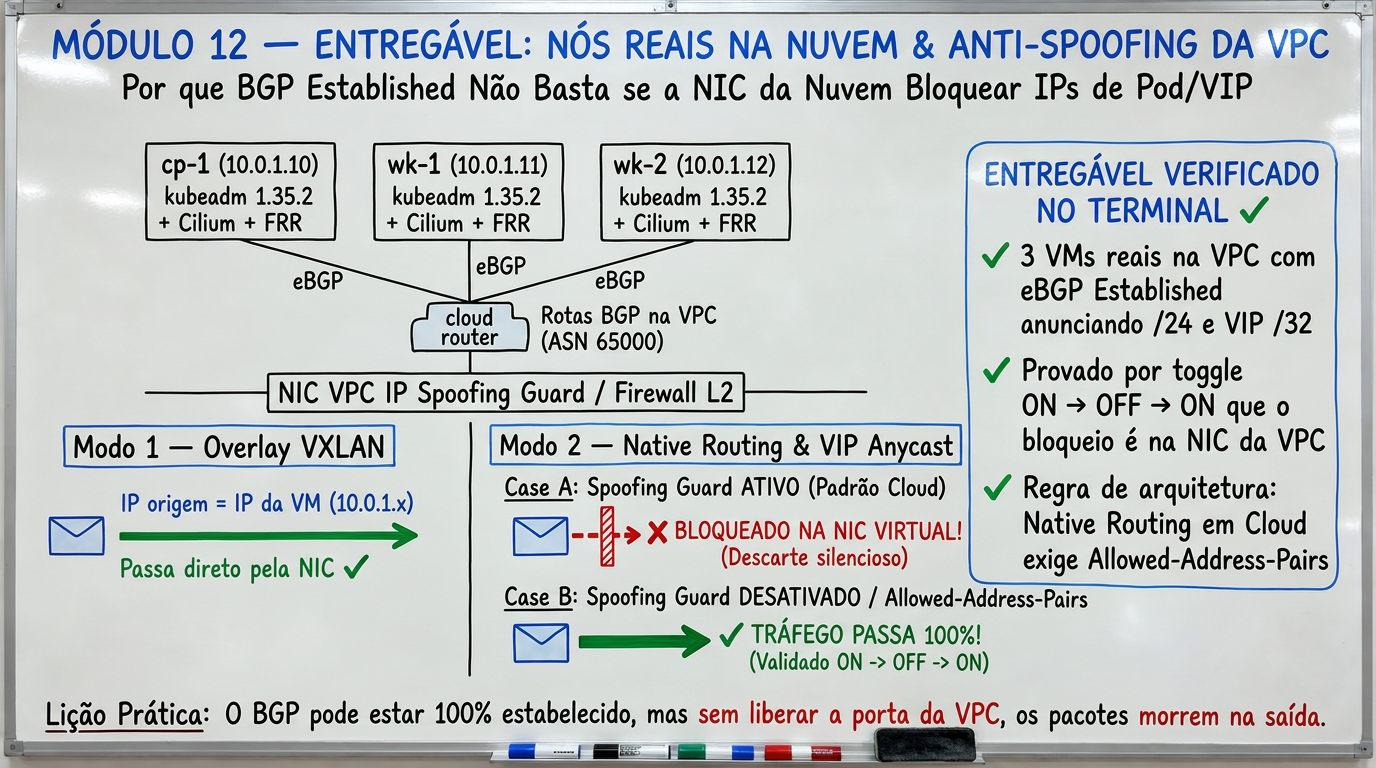
\includegraphics[width=\textwidth,height=0.72\textheight,keepaspectratio]{diagramas/m12-whiteboard-entregavel.png}
\fonte{elaborada pelo autor (2026).}
\end{figure}

Em três VMs reais da nuvem, \texttt{kubeadm} 1.35.2 sem kube-proxy e Cilium 1.20.1
funcionaram 1:1 com overlay VXLAN (MTU 1450, RTT \textasciitilde0,9 ms). Um FRR externo na
mesma VPC recebeu por eBGP os três PodCIDR \texttt{/\allowbreak{}24} e a VIP anycast \texttt{/\allowbreak{}32} com
ECMP de três next-hops: o cenário do lab reproduziu-se em fabric real.

O que a plataforma bloqueou é a lição: com o guard de spoofing de IP da porta
ligado, SYNs com origem de pod saíam da NIC e não voltavam, e pacotes com
destino que não é o IP da porta (VIP anycast, IP de pod) eram descartados
antes do nó. A prova causal foi um toggle ON→OFF→ON na porta de um único nó:
com OFF, pod direto, VIP por BGP, VIP por rota estática e conexão nova
pod→FRR sem SNAT funcionaram; com ON, apenas NodePort. A API reportou \texttt{false}
antes de o datapath aceitar; um canário FRR→pod é o único readiness confiável.

Para native routing ou VIP anycast em nós reais, a porta precisa aceitar
origens e destinos além do seu próprio IP, por allowed-address-pairs ou guard
desligado. Isso é uma decisão de postura de segurança da VPC, não um ajuste
do Cilium.

\chapter{DCI, OVN, FRR e EVPN: o que os resultados provam}\label{dci-ovn-frr-e-evpn-o-que-os-resultados-provam}

Este módulo é uma leitura guiada dos resultados históricos de \texttt{P004-{}\allowbreak{}S001} a
\texttt{P004-{}\allowbreak{}S008}, todas concluídas com \textbf{PASS}. Os perfis do \texttt{labctl} e os
artefatos de \texttt{studies/\allowbreak{}p004/\allowbreak{}} ficam no repositório como referência do
instrutor. A atividade aqui é interpretar as medições comparadas, sem depender
do estado atual da VM. A Figura 15 sintetiza o entregável do módulo.

\begin{figure}[!htbp]
\caption{Síntese visual do entregável do Módulo 13: Síntese P004 (DCI Connect,
OVN-Kubernetes + EVPN, Braços Cilium A/B + KubeVirt, R6=0 e
INV-PoC-01..06)}
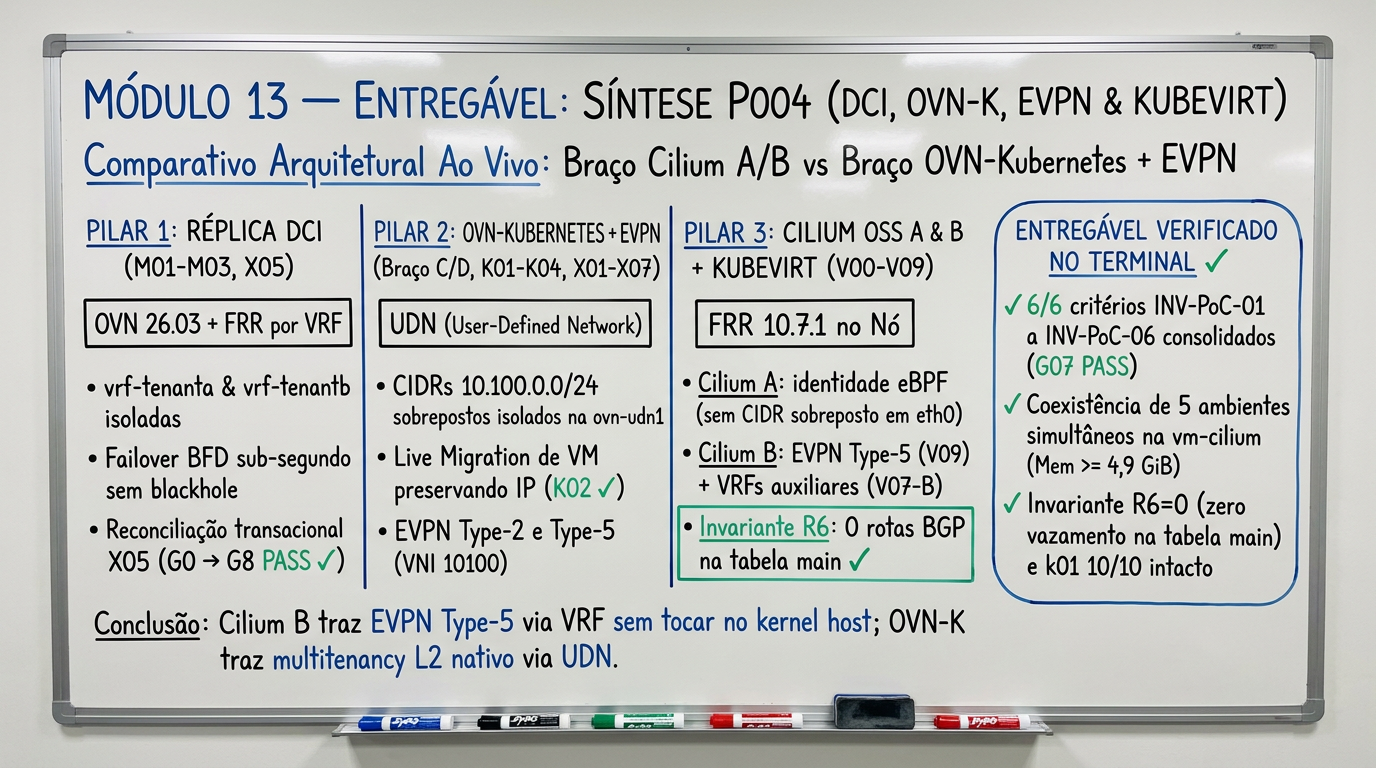
\includegraphics[width=\textwidth,height=0.72\textheight,keepaspectratio]{diagramas/m13-whiteboard-entregavel.png}
\fonte{elaborada pelo autor (2026).}
\end{figure}

\section{Plano DCI Connect (P004-S002): OVN, FRR multi-VRF e X05}\label{plano-dci-connect-p004-s002-ovn-frr-multi-vrf-e-x05}

\begin{figure}[!htbp]
\caption{Caminhos históricos da réplica DCI, com o cliente legado e o peer EVPN
separados}
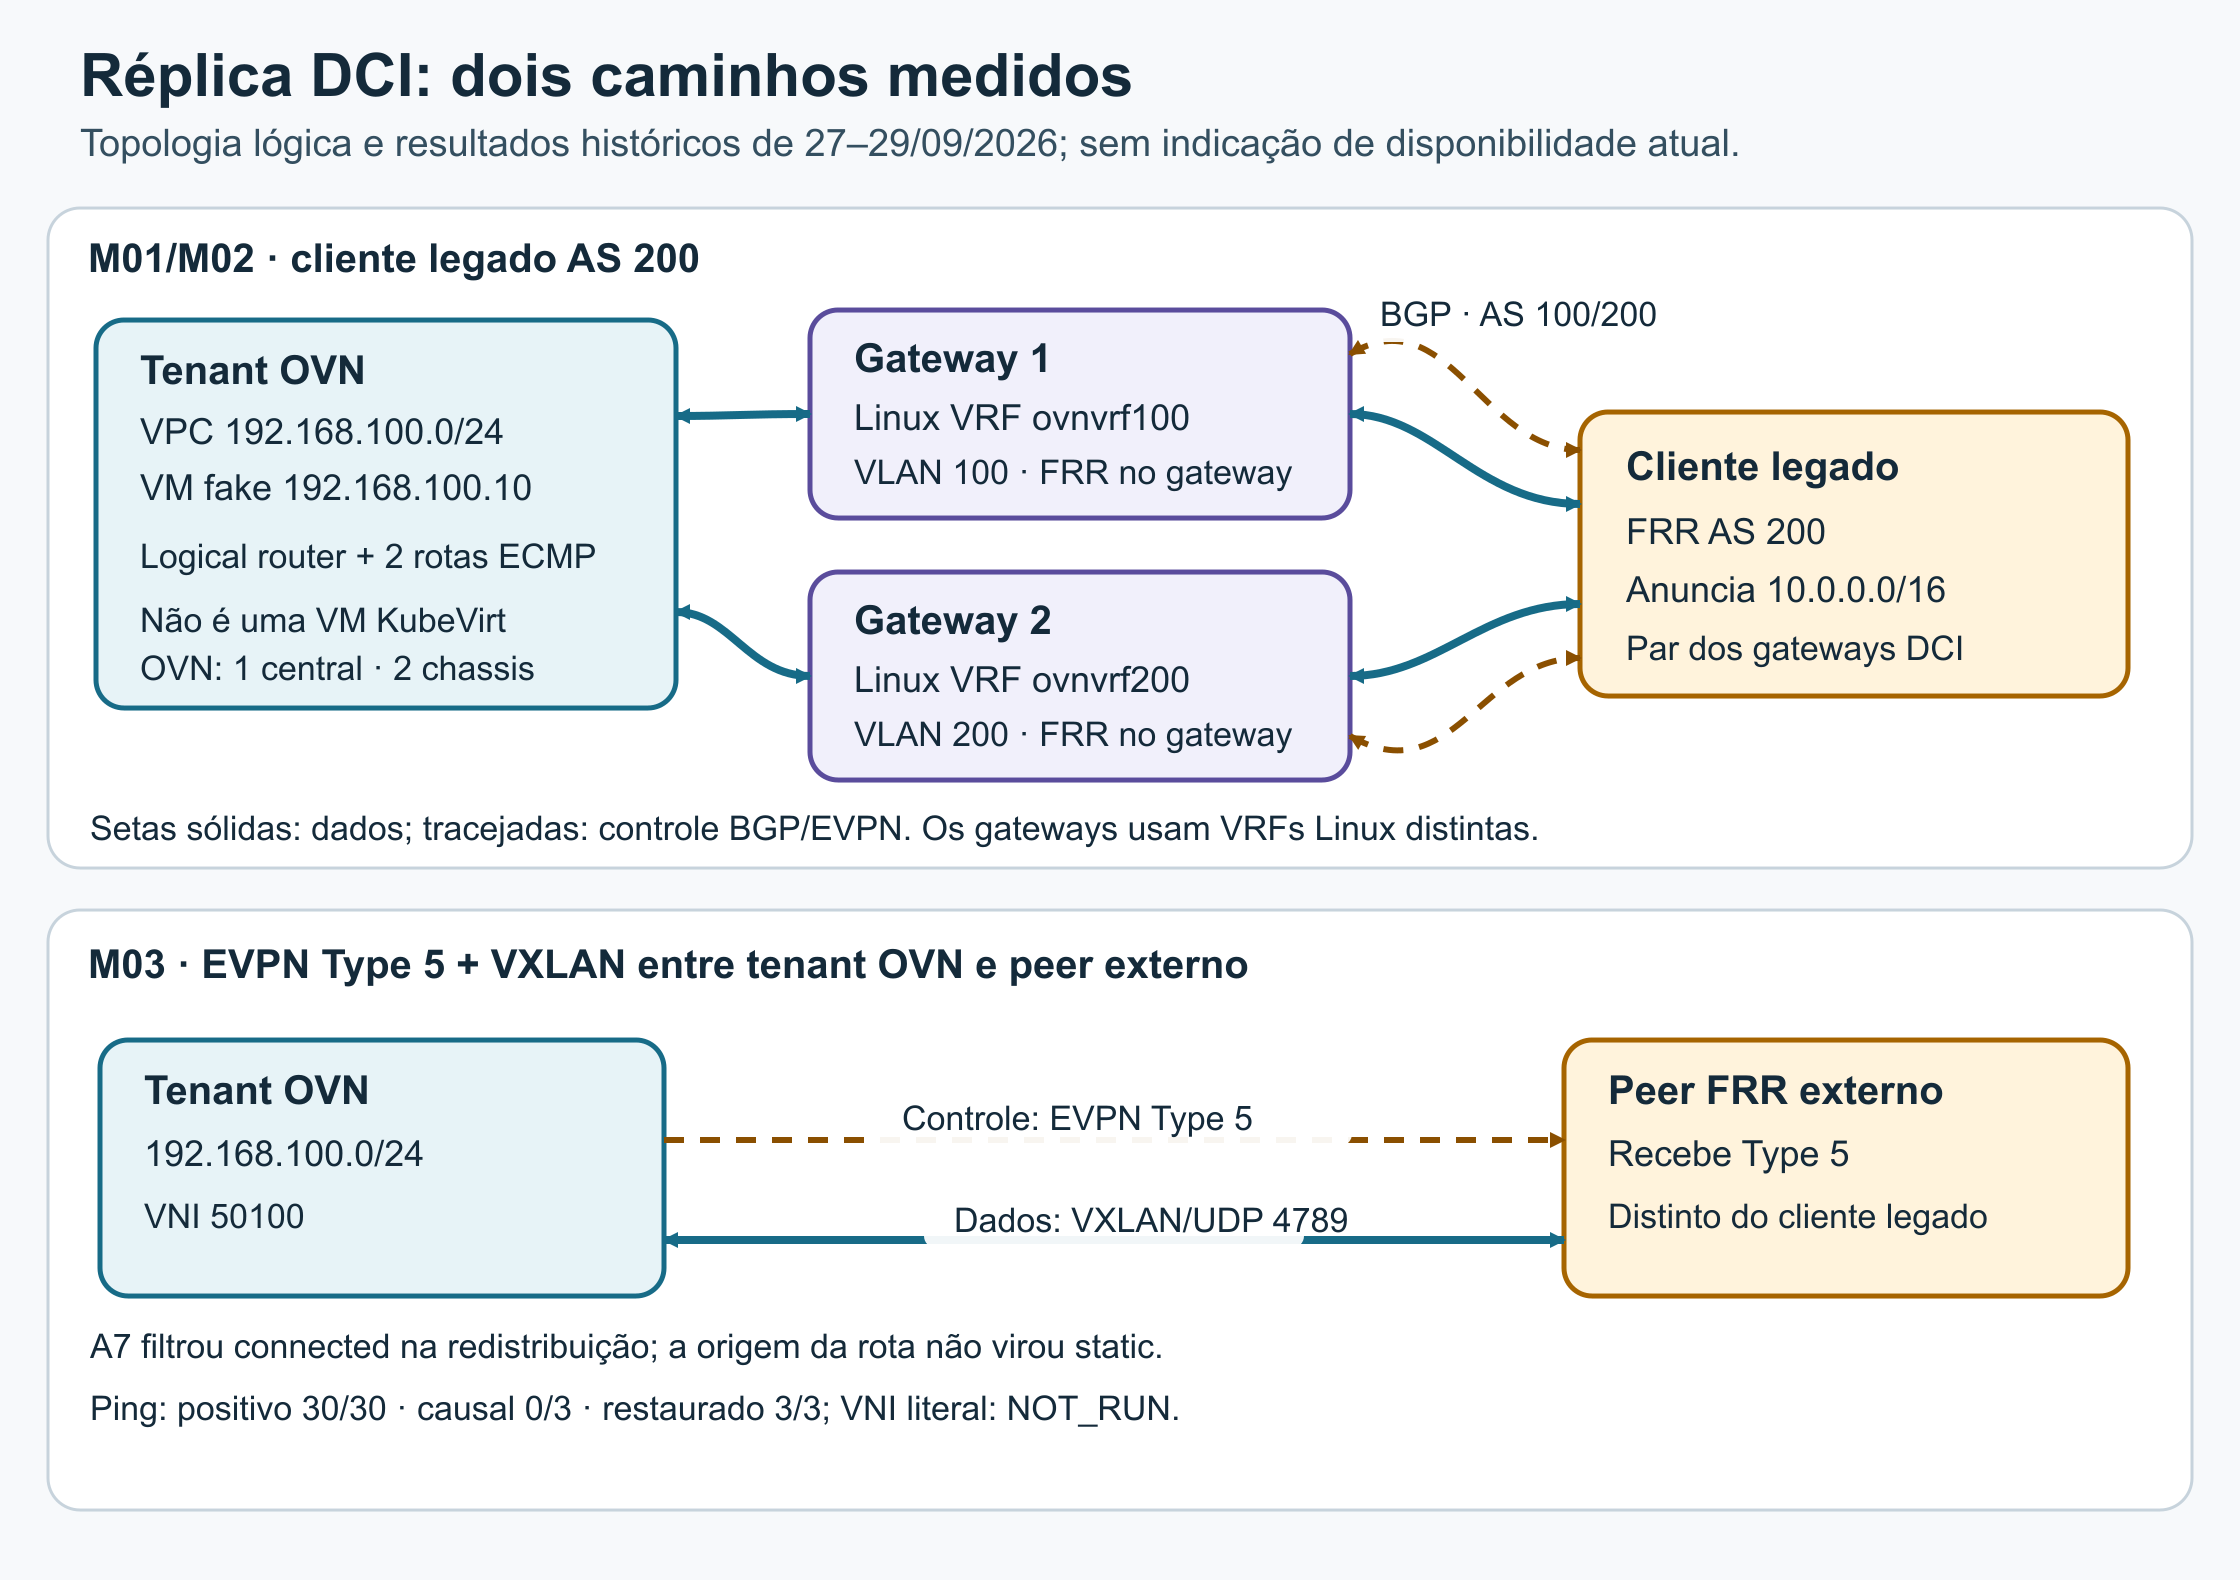
\includegraphics[width=\textwidth,height=0.72\textheight,keepaspectratio]{diagramas/07-dci-caminhos.png}
\fonte{elaborada pelo autor (2026).}
\nota{topologia lógica dos caminhos medidos na réplica DCI; o desenho não
representa um inventário ou estado operacional atual.}
\end{figure}

A réplica tem dois caminhos distintos, e cada caso usa um deles:

\begin{itemize}
\tightlist
\item
  \textbf{Caminho do cliente legado (M01 e M02):} o tenant OVN usou a rede \texttt{192.\allowbreak{}168.\allowbreak{}100.\allowbreak{}0/\allowbreak{}24}, com uma VM simulada. Dois Connect Gateways tinham as VRFs Linux \texttt{ovnvrf100} e \texttt{ovnvrf200}, com FRR dentro dos próprios gateways. Cada gateway mantinha uma sessão BGP com o cliente legado AS 200, que anunciava \texttt{10.\allowbreak{}0.\allowbreak{}0.\allowbreak{}0/\allowbreak{}16}.
\item
  \textbf{Caminho do peer EVPN (M03 e X05):} um peer externo recebeu as rotas EVPN Type 5 (Rabadan et al., 2021) dos tenants, identificadas pelo VNI 50100 (tenant A) e pelo VNI 50200 (tenant B, em X05). Esse peer não era o cliente legado das VLANs 100 e 200.
\end{itemize}

\begin{figure}[!htbp]
\caption{Estado histórico consolidado das trilhas e gates de P004 (S001 a S008
PASS)}
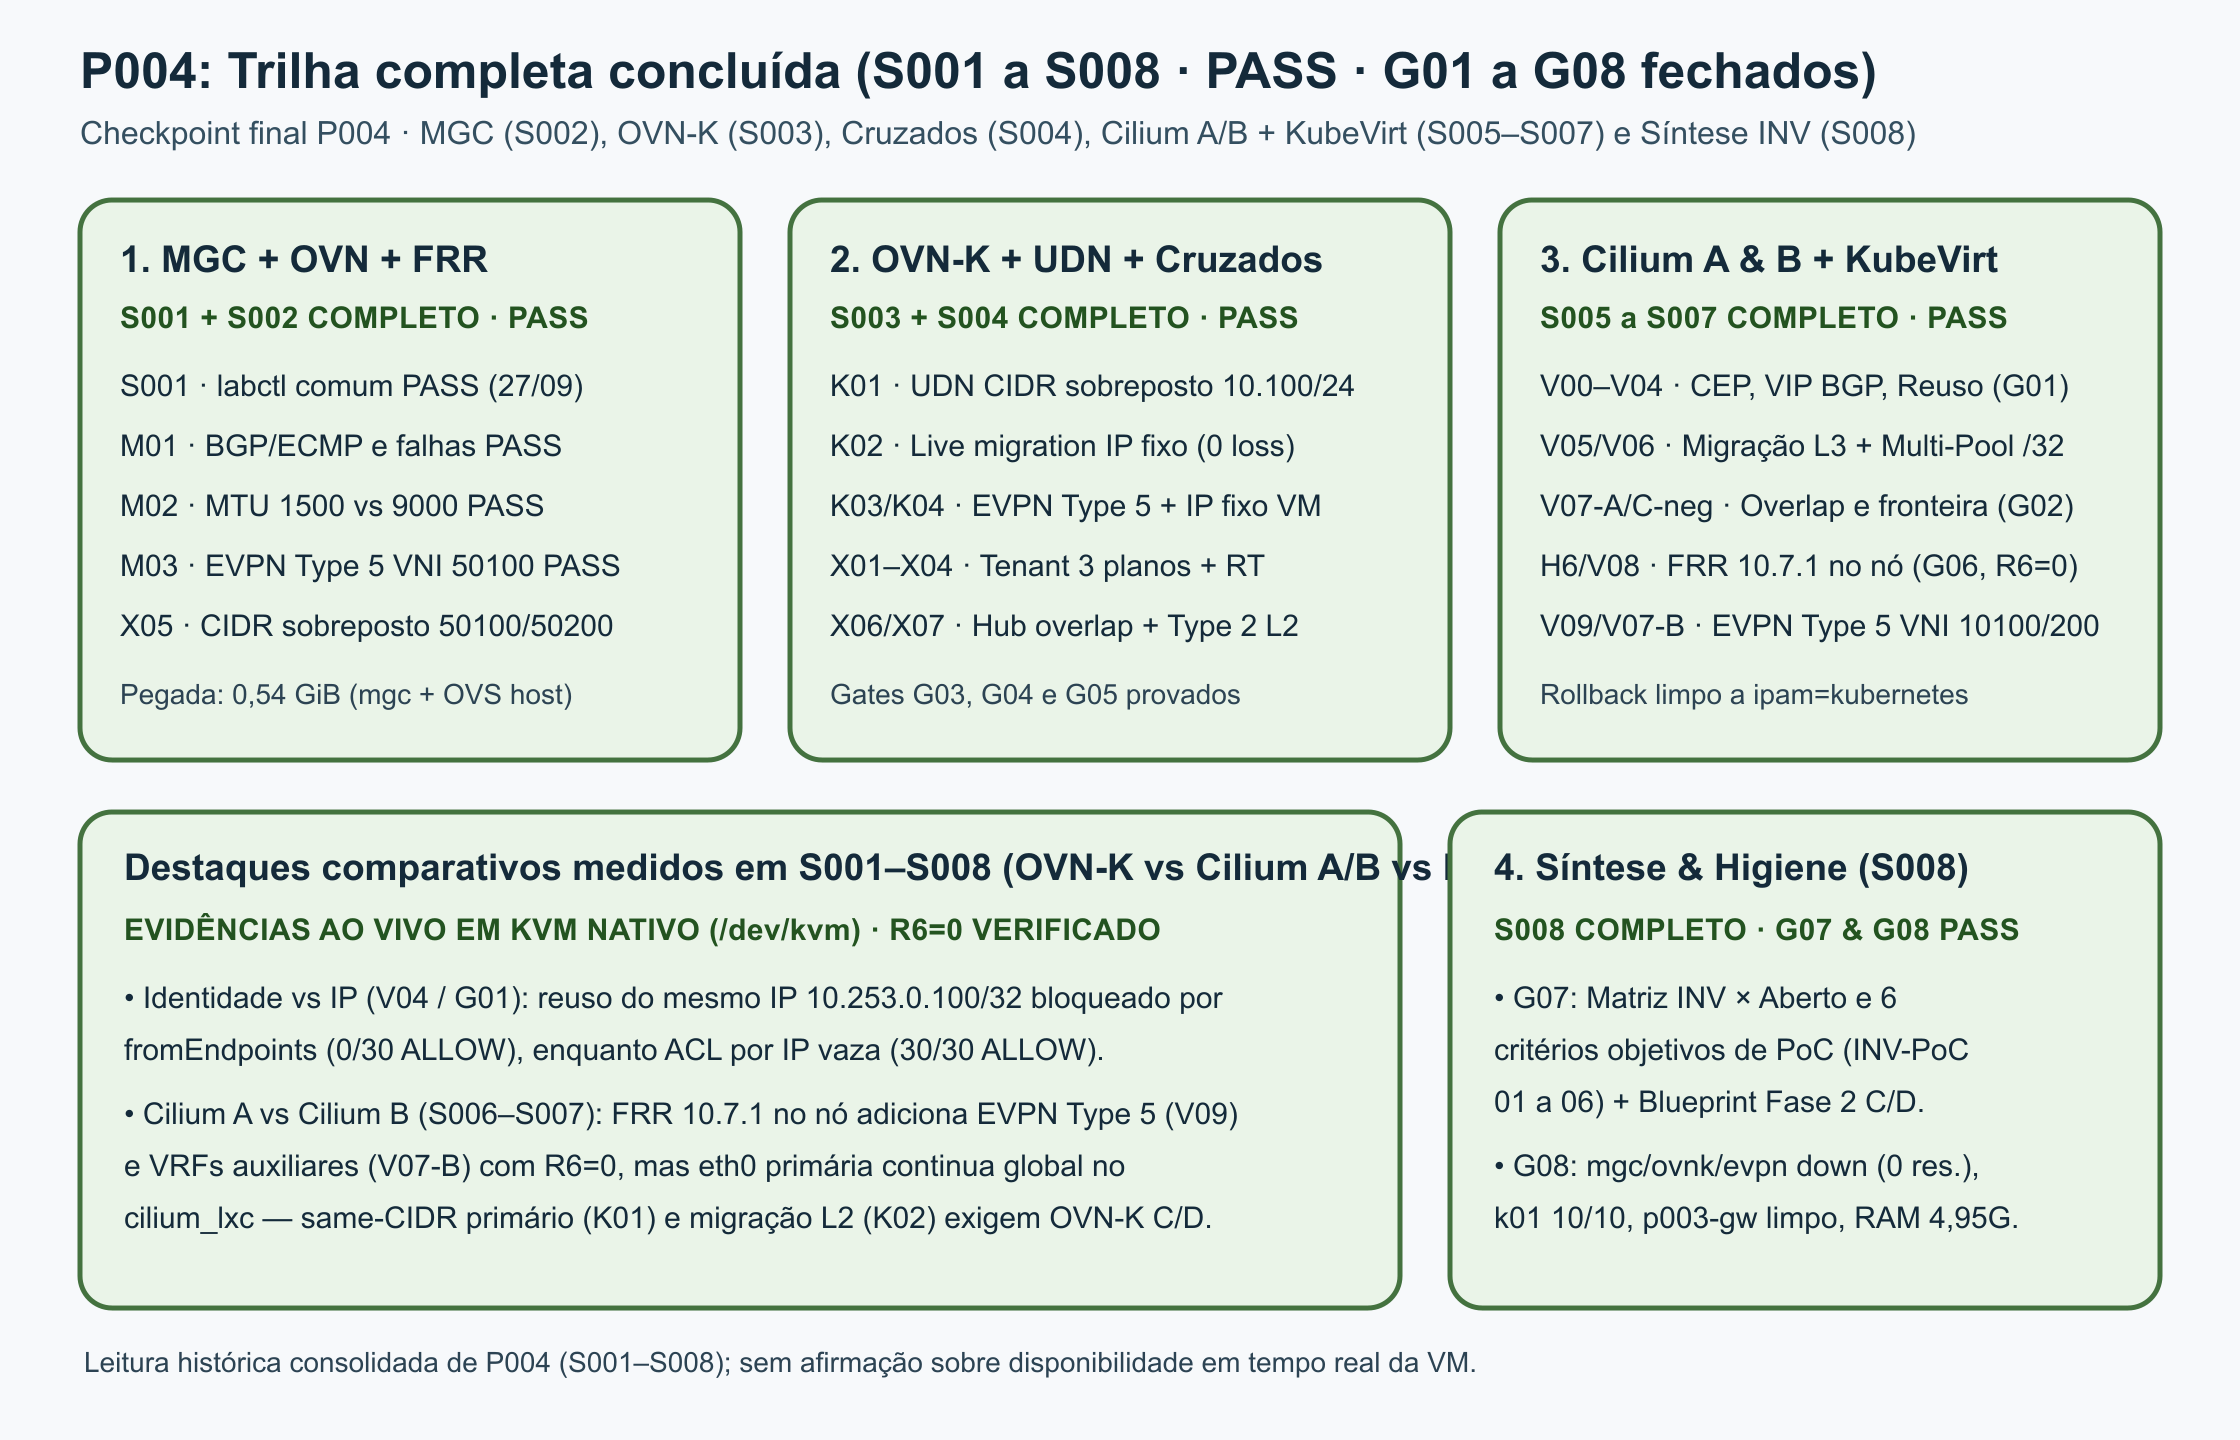
\includegraphics[width=\textwidth,height=0.72\textheight,keepaspectratio]{diagramas/08-p004-estado.png}
\fonte{elaborada pelo autor (2026).}
\nota{trilha P004 concluída com PASS de S001 a S008 (\texttt{G01} a
\texttt{G08} fechados).}
\end{figure}

Os quatro casos do plano DCI:

\begin{itemize}
\tightlist
\item
  \textbf{M01 --- falhas no plano de controle:} withdraws e falhas controladas preservaram o tráfego medido. Há uma ressalva de escopo: a falha de FRR parou \texttt{bgpd}, \texttt{bfdd} e \texttt{zebra} dentro do gateway \texttt{ovn-{}\allowbreak{}gw-{}\allowbreak{}1}, e não um contêiner FRR separado. Os gateways usaram FRR 10.7.0, e o cliente, 8.4.1\_git. A falha do chassis \texttt{ovn-{}\allowbreak{}chassis-{}\allowbreak{}1}, que hospedava a VM simulada, não foi testada.
\item
  \textbf{M02 --- MTU:} com MTU 1500, pacotes pequenos passaram 30/30, mas o pacote IPv4 jumbo de 9000 B com DF não teve resposta (0/30) e o roteador devolveu ICMP Frag Needed com MTU 1500. Com MTU 9000, pacotes pequenos e jumbo passaram 30/30. As MTUs foram restauradas a 1500 ao final. A reprodução literal da fragmentação no tap físico da PoC ficou parcial.
\item
  \textbf{M03 --- anúncio EVPN Type 5 com controle causal:} o positivo alcançou \texttt{192.\allowbreak{}168.\allowbreak{}100.\allowbreak{}0/\allowbreak{}24} como Type 5 no VNI 50100, e o ping respondeu 30/30. No controle causal, a chave \texttt{dynamic-{}\allowbreak{}routing-{}\allowbreak{}redistribute=\allowbreak{}static} na LRP do tenant excluiu as rotas \texttt{connected} dos anúncios. Com isso, a rota saiu do SB, da tabela do tenant, do Type 5 e da FIB, e o ping teve 0/3 respostas; BGP e VTEP continuaram ativos. Ao remover a chave, o ping voltou a 3/3. O controle negativo literal do VNI ficou NOT\_RUN, por falta de causalidade com o withdraw da rota.
\item
  \textbf{X05 --- dois tenants com a mesma sub-rede:} concluído com \textbf{PASS} em 23/10/2026. O tenant B reutilizou a sub-rede \texttt{192.\allowbreak{}168.\allowbreak{}100.\allowbreak{}0/\allowbreak{}24} e o mesmo \texttt{/\allowbreak{}30} de trânsito \texttt{169.\allowbreak{}254.\allowbreak{}254.\allowbreak{}0/\allowbreak{}30}, isolado no VRF \texttt{ovnvrf50200} (VNI 50200). O alcance dentro de cada tenant passou 30/30, e as quatro direções entre tenants tiveram 0/3 respostas, sem nenhum pacote capturado no destino. Para o peer desencapsular o Type 5, o \texttt{Router MAC} anunciado precisou coincidir com o MAC de \texttt{br-{}\allowbreak{}vxlan50200}. O rollback retirou primeiro os anúncios BGP/EVPN e depois os objetos OVN e os VRFs, sem deixar resíduos.
\end{itemize}

\section{OVN-Kubernetes, UDN/EVPN, KubeVirt e casos cruzados (P004-S003 e P004-S004)}\label{ovn-kubernetes-udnevpn-kubevirt-e-casos-cruzados-p004-s003-e-p004-s004}

\begin{figure}[!htbp]
\caption{Arquitetura comparada de P004 (S002 a S008): OVN-K, Fabric EVPN e Braços
Cilium A e B + KubeVirt}
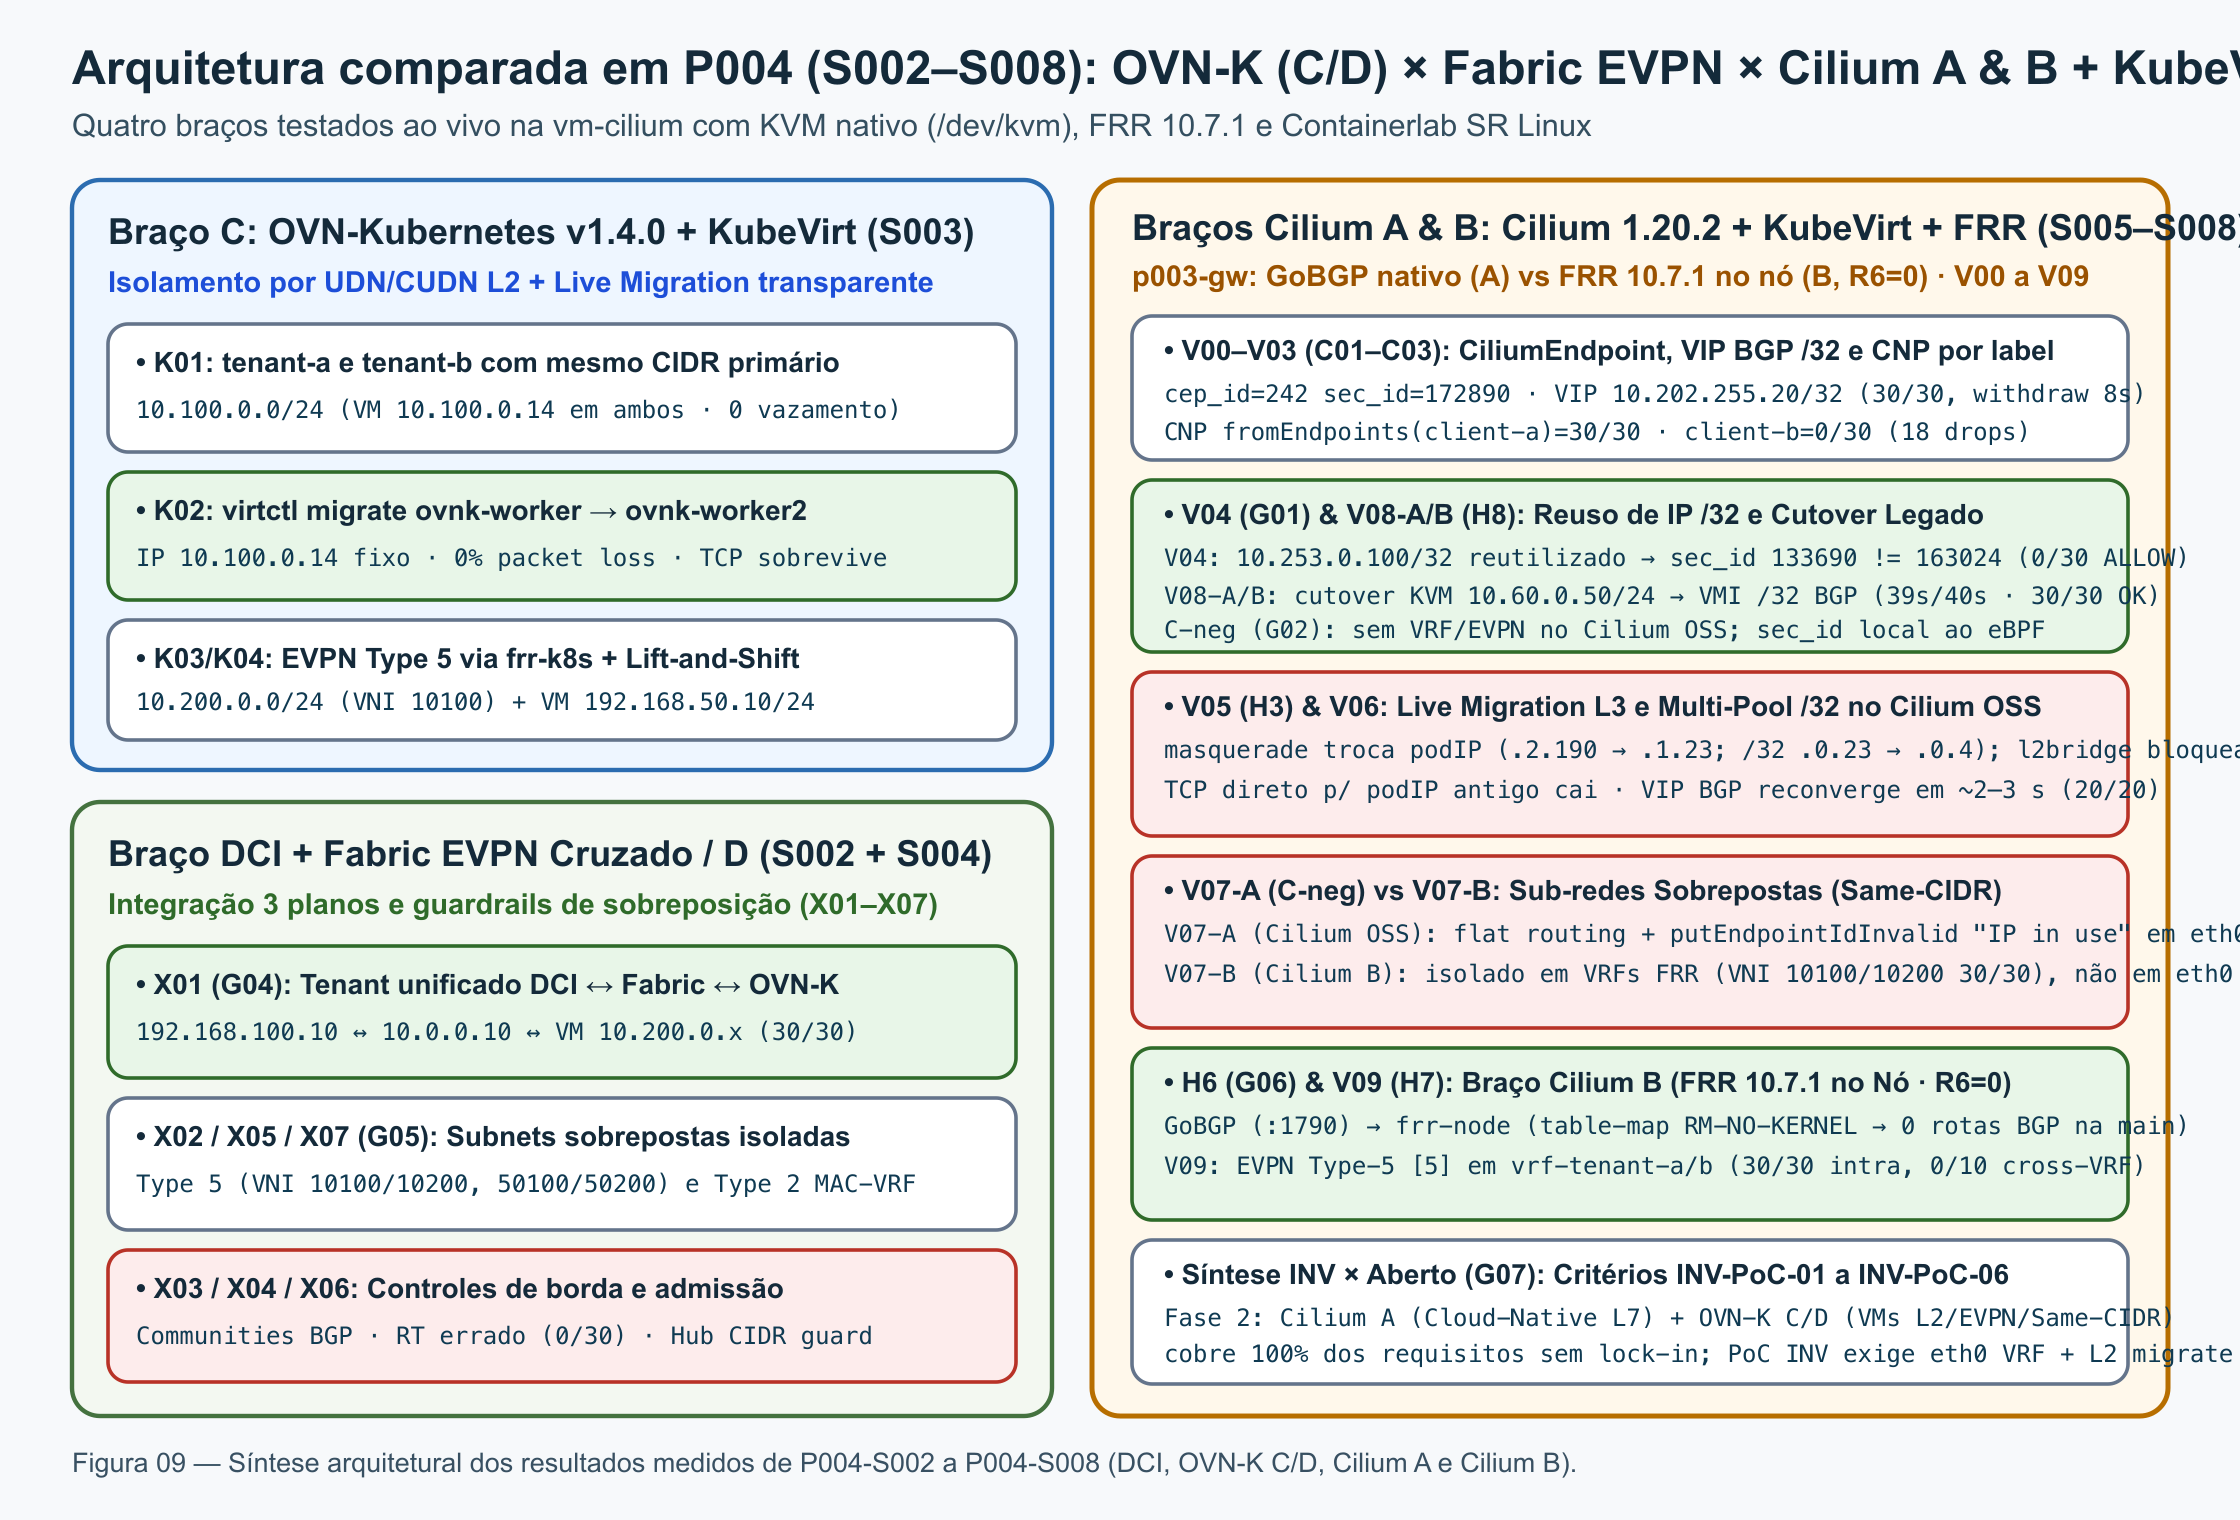
\includegraphics[width=\textwidth,height=0.72\textheight,keepaspectratio]{diagramas/09-p004-tres-planos-kubevirt.png}
\fonte{elaborada pelo autor (2026).}
\nota{comparação experimental entre os braços testados em P004-S002 a
P004-S008 com KVM nativo (\texttt{/\allowbreak{}dev/\allowbreak{}kvm}),
EVPN, Cilium 1.20.2 e FRR 10.7.1 (\texttt{R6=\allowbreak{}0}).}
\end{figure}

A sessão \texttt{P004-{}\allowbreak{}S003} (\textbf{PASS} em 23/10/2026) subiu um cluster kind de 3 nós
com OVN-Kubernetes \texttt{v1.\allowbreak{}4.\allowbreak{}0} (OVN-Kubernetes, {[}2026{]}), KubeVirt \texttt{v1.\allowbreak{}9.\allowbreak{}0}
(KubeVirt, {[}2026{]}) em KVM nativo e \texttt{frr-{}\allowbreak{}k8s} \texttt{v0.\allowbreak{}0.\allowbreak{}27}. Ela provou o gate
\textbf{\texttt{G03}} com quatro casos:

\begin{itemize}
\tightlist
\item
  \textbf{K01 --- CIDR sobreposto:} duas \texttt{User\allowbreak{}Defined\allowbreak{}Network} primárias usaram o mesmo CIDR \texttt{10.\allowbreak{}100.\allowbreak{}0.\allowbreak{}0/\allowbreak{}24}. As VMs dos dois tenants receberam o \textbf{mesmo IP \texttt{10.\allowbreak{}100.\allowbreak{}0.\allowbreak{}14}}, responderam 30/30 dentro do próprio tenant e tiveram 0/30 entre tenants.
\item
  \textbf{K02 --- live migration:} \texttt{virtctl migrate} moveu a VM entre dois workers em \textasciitilde16 s. O IP \texttt{10.\allowbreak{}100.\allowbreak{}0.\allowbreak{}14/\allowbreak{}24} foi preservado, a perda ICMP foi de \textbf{0\%} (60/60) e a \textbf{sessão TCP longa sobreviveu}.
\item
  \textbf{K03 e K04 --- EVPN Type 5 e lift-and-shift:} uma \texttt{Cluster\allowbreak{}User\allowbreak{}Defined\allowbreak{}Network} (\texttt{10.\allowbreak{}200.\allowbreak{}0.\allowbreak{}0/\allowbreak{}24}) foi anunciada ao fabric EVPN via \texttt{Route\allowbreak{}Advertisements} e \texttt{frr-{}\allowbreak{}k8s} (VNI 10100), com 30/30 no positivo e 0/10 no negativo. O K04 preservou o IP fixo legado \texttt{192.\allowbreak{}168.\allowbreak{}50.\allowbreak{}10/\allowbreak{}24}.
\end{itemize}

A sessão \texttt{P004-{}\allowbreak{}S004} (\textbf{PASS} em 24/10/2026) integrou os planos \texttt{dci},
\texttt{evpn-{}\allowbreak{}fabric} e \texttt{ovnk} com KubeVirt ao mesmo tempo e provou os gates \textbf{\texttt{G04}} e
\textbf{\texttt{G05}}:

\begin{itemize}
\tightlist
\item
  \textbf{X01 --- conectividade do tenant unificado:} 30/30 fim a fim.
\item
  \textbf{X02 --- isolamento em três planos:} com \texttt{10.\allowbreak{}200.\allowbreak{}0.\allowbreak{}0/\allowbreak{}24} e \texttt{10.\allowbreak{}0.\allowbreak{}0.\allowbreak{}0/\allowbreak{}24} sobrepostos, nenhum pacote vazou.
\item
  \textbf{X03 e X04 --- filtros:} a filtragem por BGP community funcionou, e um Route-Target incorreto bloqueou o tráfego (0/30).
\item
  \textbf{X06 e X07 --- colisão e extensão L2:} o X06 detectou colisão de CIDR em VRF hub. O X07 estendeu L2 em \texttt{MAC-{}\allowbreak{}VRF} EVPN Type 2 (Sajassi et al., 2015) com o mesmo CIDR \texttt{172.\allowbreak{}16.\allowbreak{}50.\allowbreak{}0/\allowbreak{}24} em VNIs diferentes (20100 e 20200).
\end{itemize}

\section{Braço Cilium A: Cilium 1.20.2 com KubeVirt v1.9.0 (P004-S005)}\label{brauxe7o-cilium-a-cilium-1.20.2-com-kubevirt-v1.9.0-p004-s005}

A sessão \texttt{P004-{}\allowbreak{}S005} (\textbf{PASS} em 24/10/2026) instalou o KubeVirt \texttt{v1.\allowbreak{}9.\allowbreak{}0} no
sandbox \texttt{p003-{}\allowbreak{}gw}, com Cilium 1.20.2. Antes, os perfis \texttt{ovnk}, \texttt{evpn-{}\allowbreak{}fabric} e
\texttt{dci} foram desligados para cumprir \texttt{Mem\allowbreak{}Available \textgreater{}=\allowbreak{} 4 Gi\allowbreak{}B}. Os casos
\texttt{V00}--\texttt{V06} foram medidos ao vivo:

\begin{itemize}
\tightlist
\item
  \textbf{V00 e V01 --- datapath da VM:} uma VM CirrOS sobre \texttt{/\allowbreak{}dev/\allowbreak{}kvm} comunicou-se com pods nos dois sentidos (30/30); com a VM parada, 0/30. No Cilium, o pod \texttt{virt-{}\allowbreak{}launcher} aparece como um \texttt{Cilium\allowbreak{}Endpoint} comum, com IP do PodCIDR do nó, enquanto o guest usa um endereço interno próprio.
\item
  \textbf{V02 e V03 --- VIP BGP e política:} um \texttt{Service} LoadBalancer da VM foi anunciado por BGP (\texttt{10.\allowbreak{}202.\allowbreak{}255.\allowbreak{}20/\allowbreak{}32}) e respondeu 30/30 ao cliente externo; após o withdraw, caiu para 0/30 em 8 s. Uma \texttt{Cilium\allowbreak{}Network\allowbreak{}Policy} por label permitiu 30/30 do cliente autorizado e bloqueou o outro (0/30), com 18 drops \texttt{Policy denied}.
\item
  \textbf{V04 --- reuso de IP versus identidade (gate \texttt{G01}):} um pool de IP único (\texttt{10.\allowbreak{}253.\allowbreak{}0.\allowbreak{}100/\allowbreak{}32}) forçou duas VMs a usar o mesmo IP, uma após a outra. A primeira obteve 30/30. A segunda herdou o IP, mas recebeu outra identidade de segurança e obteve \textbf{0/30} sob \texttt{from\allowbreak{}Endpoints}, com 25 drops \texttt{Policy denied}. Já uma ACL baseada só no IP concedeu 30/30 à segunda VM.
\item
  \textbf{V05 --- live migration no Cilium OSS:} a migração entre workers levou 22 s, trocou o IP do \texttt{virt-{}\allowbreak{}launcher} e derrubou a sessão TCP aberta para o IP antigo. A VIP BGP \texttt{10.\allowbreak{}202.\allowbreak{}255.\allowbreak{}20/\allowbreak{}32} reconvergiu sozinha, com intervalo máximo de 3000.0ms.
\item
  \textbf{V06 --- Multi-Pool \texttt{/\allowbreak{}32} com migração:} com \texttt{ipam.\allowbreak{}mode=\allowbreak{}multi-{}\allowbreak{}pool} e \texttt{mask\allowbreak{}Size:\allowbreak{} 32}, a VM recebeu \texttt{10.\allowbreak{}252.\allowbreak{}0.\allowbreak{}23/\allowbreak{}32} e respondeu 30/30 a probes diretos. Após migrar, recebeu \texttt{10.\allowbreak{}252.\allowbreak{}0.\allowbreak{}4/\allowbreak{}32} (30/30), enquanto o bloco antigo ficou retido no nó de origem pelo piso \texttt{multi\allowbreak{}Pool\allowbreak{}Pre\allowbreak{}Allocation}. O rollback devolveu o cluster a \texttt{ipam.\allowbreak{}mode=\allowbreak{}kubernetes} sem pools residuais.
\end{itemize}

\section{Negativos do Braço A, Braço Cilium B e síntese INV × aberto (P004-S006 a P004-S008)}\label{negativos-do-brauxe7o-a-brauxe7o-cilium-b-e-suxedntese-inv-aberto-p004-s006-a-p004-s008}

As sessões \texttt{P004-{}\allowbreak{}S006} a \texttt{P004-{}\allowbreak{}S008} (\textbf{PASS}) fecharam a comparação entre
\textbf{Cilium A}, \textbf{Cilium B}, \textbf{OVN-Kubernetes (\texttt{C/\allowbreak{}D})} e \textbf{INV}.

Limites do Braço Cilium A (\texttt{P004-{}\allowbreak{}S006}, gate \texttt{G02}):

\begin{itemize}
\tightlist
\item
  \textbf{V07-A --- sub-redes sobrepostas:} dois namespaces com o mesmo CIDR caem na mesma tabela de roteamento, sem isolamento L3 (\texttt{vrf\_\allowbreak{}count=\allowbreak{}0}). Dois pods que pedem o mesmo IP \texttt{/\allowbreak{}32} no mesmo nó falham no segundo, com \texttt{is already in use}, por colisão no mapa BPF global \texttt{cilium\_\allowbreak{}lxc}.
\item
  \textbf{V08-A --- cutover de VM legada:} uma VM QEMU/KVM legada (30/30 HTTP) foi substituída por uma VM KubeVirt que anuncia o mesmo IP como \texttt{10.\allowbreak{}60.\allowbreak{}0.\allowbreak{}50/\allowbreak{}32}. O \texttt{/\allowbreak{}32} prevaleceu sobre o \texttt{/\allowbreak{}24} no \texttt{border1} em 25 s, e o cutover completo levou 39 s, com 30/30 HTTP.
\item
  \textbf{C-neg --- o que a API BGP do Cilium não aceita:} a API BGP v2 rejeita \texttt{vrf}, \texttt{evpn} e \texttt{l2vpn} (\texttt{strict decoding error}), não instala rotas recebidas no kernel (\texttt{proto bgp =\allowbreak{} 0}) e não leva a identidade eBPF no cabeçalho IP externo.
\end{itemize}

Braço Cilium B, com FRR 10.7.1 no nó sob o invariante \texttt{R6=\allowbreak{}0} (\texttt{P004-{}\allowbreak{}S006} e
\texttt{P004-{}\allowbreak{}S007}):

\begin{itemize}
\tightlist
\item
  \textbf{H6 --- FRR ao lado do Cilium (gate \texttt{G06}):} um \texttt{Daemon\allowbreak{}Set} com FRR 10.7.1 pareia com o GoBGP do Cilium e com os switches ToR. O \texttt{table-{}\allowbreak{}map RM-{}\allowbreak{}NO-{}\allowbreak{}KERNEL} mantém \textbf{zero rotas BGP} na tabela \texttt{main}, protegendo o datapath eBPF.
\item
  \textbf{V09 e V07-B --- EVPN Type 5 em VRFs do nó:} em VRFs Linux do nó (VNIs 10100 e 10200), o FRR anuncia e importa rotas EVPN Type 5 e isola CIDRs e IPs idênticos: 30/30 dentro do VRF, 0/10 entre VRFs, com \texttt{R6=\allowbreak{}0}. A interface primária \texttt{eth0} dos pods e VMs, porém, continua presa ao mapa global \texttt{cilium\_\allowbreak{}lxc}.
\item
  \textbf{V08-B --- cutover via FRR no nó:} o mesmo cutover de \texttt{10.\allowbreak{}60.\allowbreak{}0.\allowbreak{}50/\allowbreak{}32}, agora pelo caminho GoBGP do Cilium → FRR no nó → \texttt{border1}, levou 40 s no total, com 30/30 HTTP e \texttt{R6=\allowbreak{}0}.
\end{itemize}

Síntese e higiene final (\texttt{P004-{}\allowbreak{}S008}, gates \texttt{G07} e \texttt{G08}):

\begin{itemize}
\tightlist
\item
  \textbf{Combinação aberta:} o blueprint da Fase 2 mostra que Cilium A, para clusters cloud-native e L7, somado ao OVN-Kubernetes \texttt{C/\allowbreak{}D}, para clusters KubeVirt com CIDR sobreposto (K01), live migration L2 (K02) e EVPN Type-2/Type-5 (K03, X01, X07), atende 100\% dos requisitos sem lock-in.
\item
  \textbf{Avaliação comercial:} uma PoC do \textbf{INV} deve ser julgada pelos seis critérios objetivos \texttt{INV-{}\allowbreak{}Po\allowbreak{}C-{}\allowbreak{}01} a \texttt{INV-{}\allowbreak{}Po\allowbreak{}C-{}\allowbreak{}06}, documentados em \texttt{20-{}\allowbreak{}dci-{}\allowbreak{}estado-{}\allowbreak{}parcial.\allowbreak{}md} §4.2.
\end{itemize}

\section{Exercícios de interpretação}\label{exercuxedcios-de-interpretauxe7uxe3o}

\begin{enumerate}
\def\labelenumi{\arabic{enumi}.}
\tightlist
\item
  Por que a limitação ``sem VRF'' dos módulos Cilium OSS não descreve o braço DCI (\texttt{S002}) nem o plano OVN-Kubernetes (\texttt{S003–S004})?
\item
  Por que a Live Migration preservou o IP \texttt{10.\allowbreak{}100.\allowbreak{}0.\allowbreak{}14} e a sessão TCP no OVN-Kubernetes (\texttt{K02}), mas trocou o IP do \texttt{virt-{}\allowbreak{}launcher} no Cilium OSS (\texttt{V05} e \texttt{V06})?
\item
  Como \texttt{V04} provou com o pool de IP único \texttt{10.\allowbreak{}253.\allowbreak{}0.\allowbreak{}100/\allowbreak{}32} que \texttt{from\allowbreak{}Endpoints} revoga o acesso no reuso de IP entre duas VMs, ao contrário de uma regra baseada apenas no endereço IP?
\item
  Por que o \texttt{table-{}\allowbreak{}map RM-{}\allowbreak{}NO-{}\allowbreak{}KERNEL} (invariante \texttt{R6=\allowbreak{}0}) é indispensável no Braço Cilium B (\texttt{H6}/\texttt{V09}), e por que mesmo com FRR \texttt{10.\allowbreak{}7.\allowbreak{}1} no nó a interface primária \texttt{eth0} do Cilium não suporta \texttt{same-{}\allowbreak{}CIDR} entre dois tenants (\texttt{V07-{}\allowbreak{}A} vs \texttt{V07-{}\allowbreak{}B})?
\end{enumerate}

As respostas comentadas, a matriz comparativa completa (\texttt{Cilium A} × \texttt{Cilium B} × \texttt{OVN-{}\allowbreak{}K C/\allowbreak{}D} × \texttt{INV}), os critérios de aceite \texttt{INV-{}\allowbreak{}Po\allowbreak{}C-{}\allowbreak{}01} a \texttt{INV-{}\allowbreak{}Po\allowbreak{}C-{}\allowbreak{}06} (\texttt{G07}) e o mapa de evidências estão em DCI, OVN-K e Cilium + KubeVirt em P004: consolidação completa de S001--S008.

\chapter{Estudos avançados P005: conexão dedicada eBGP e datapath eBPF}\label{estudos-avanuxe7ados-p005-conexuxe3o-dedicada-ebgp-e-datapath-ebpf}

A trilha P005 reúne 16 estudos (\texttt{E09}--\texttt{E19} e \texttt{E21}--\texttt{E25}), executados em
quatro ondas. Cada onda tem dois braços: o Braço A trata da borda eBGP de uma
conexão dedicada (Direct Connect), e o Braço B, do datapath eBPF, da escala e
da observabilidade. A Figura 19 sintetiza o entregável do módulo.

\begin{figure}[!htbp]
\caption{Síntese visual do entregável do Módulo 14: Estudos Avançados P005 (16/16
PASS --- Borda eBGP Dedicada ∥ Datapath eBPF, Observabilidade e DRA)}
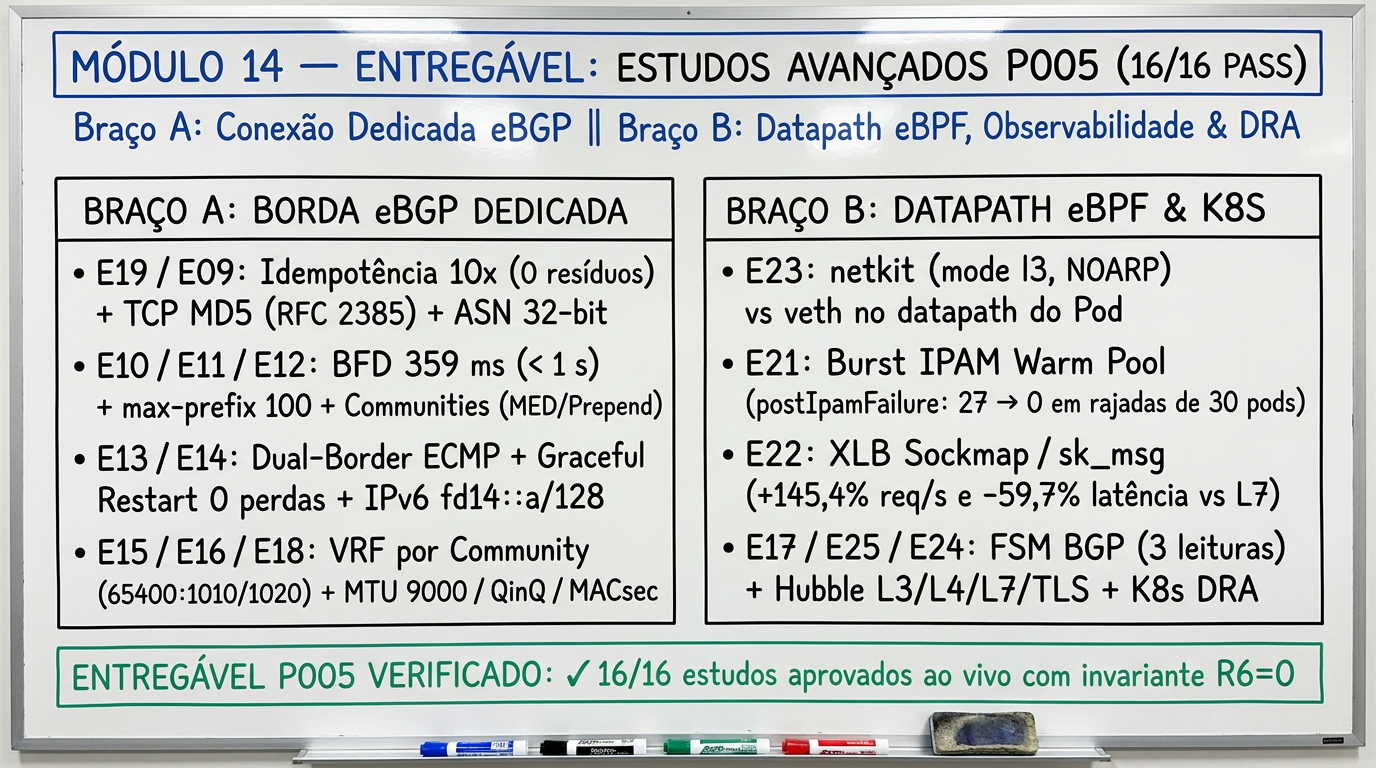
\includegraphics[width=\textwidth,height=0.72\textheight,keepaspectratio]{diagramas/m14-whiteboard-entregavel.png}
\fonte{elaborada pelo autor (2026).}
\end{figure}

\section{Onda 1 (P005-S001): idempotência BGP, TCP MD5, netkit e burst IPAM}\label{onda-1-p005-s001-idempotuxeancia-bgp-tcp-md5-netkit-e-burst-ipam}

Onda concluída com \textbf{PASS}; estudos \texttt{E19}, \texttt{E09}, \texttt{E23} e \texttt{E21}. O \texttt{E09} aplica a autenticação TCP MD5 da RFC 2385 (Heffernan, 1998).

\begin{itemize}
\tightlist
\item
  \textbf{Braço A, conexão dedicada eBGP (\texttt{19-{}\allowbreak{}bgp-{}\allowbreak{}idempotency-{}\allowbreak{}md5-{}\allowbreak{}asn32.\allowbreak{}md}):}

  \begin{itemize}
  \tightlist
  \item
    \textbf{E19 --- idempotência BGP e reuso de VIP:} o estudo aplicou 10 vezes seguidas os mesmos recursos BGP com \texttt{kubectl apply}. O resultado foi \textbf{0 diferenças} nas políticas, nas rotas anunciadas e na RIB do \texttt{border1}. Ou seja, um loop de GitOps não gera flaps nem \texttt{UPDATE}s espúrios. A remoção limpou 100\% das rotas em 11 s, com \texttt{R6=\allowbreak{}0}, e a mesma VIP, reaproveitada por outro Service, respondeu 30/30 HTTP 200 sem nenhuma resposta antiga.
  \item
    \textbf{E09 --- sessão eBGP com TCP MD5 e ASN de 32 bits:} um nó do cluster formou sessão autenticada por \texttt{auth\allowbreak{}Secret\allowbreak{}Ref} com um roteador FRR de ASN 4200000001. A sessão convergiu em 3 s, e o \texttt{tcpdump} mostrou a opção TCP 19 (MD5). Uma senha errada derrubou apenas o peer inválido, sem afetar as 3/3 sessões do fabric. Um \texttt{Secret} ausente falhou de forma segura, e a troca de senha em produção restabeleceu a sessão em \textbf{9,39 s}.
  \end{itemize}
\item
  \textbf{Braço B, datapath eBPF e escala de alocação (\texttt{21-{}\allowbreak{}netkit-{}\allowbreak{}vs-{}\allowbreak{}veth-{}\allowbreak{}ipam-{}\allowbreak{}burst.\allowbreak{}md}):}

  \begin{itemize}
  \tightlist
  \item
    \textbf{E23 --- \texttt{netkit} contra \texttt{veth}:} o estudo comparou os dois tipos de interface de pod no Cilium \texttt{1.\allowbreak{}20.\allowbreak{}2} com kernel 6.8. O \texttt{cilium-{}\allowbreak{}agent} recusou a troca enquanto havia pods \texttt{veth} ativos no nó, o que é uma proteção fail-closed. Com os pods recriados em \texttt{netkit}, o \texttt{iperf3} \textbf{eliminou 100\% das retransmissões TCP} (\texttt{47 -{}\allowbreak{}\textgreater{} 0} no mesmo nó, \texttt{11 -{}\allowbreak{}\textgreater{} 0} entre nós). Os softirqs \texttt{NET\_\allowbreak{}RX} caíram \textbf{-8,9\%} no mesmo nó e \textbf{-20,5\%} entre nós, e a \texttt{Cilium\allowbreak{}Network\allowbreak{}Policy} continuou bloqueando o tráfego proibido.
  \item
    \textbf{E21 --- rajada de pods e pool pré-aquecido:} o estudo criou 16 pods ao mesmo tempo em três configurações de IPAM. O modo \texttt{kubernetes} convergiu em 5,40 s, sem falhas. O \texttt{multi-{}\allowbreak{}pool} sem reserva sofreu \textbf{27 falhas} de alocação enquanto o operador criava blocos. Com o pool pré-aquecido por \texttt{multi\allowbreak{}Pool\allowbreak{}Pre\allowbreak{}Allocation}, as falhas caíram de 27 para 0 (-100\%). No controle negativo, um pool \texttt{/\allowbreak{}29}, com 6 IPs para 10 pods, deixou \texttt{6 Running} e \texttt{4 Pending} sem afetar os outros pools.
  \end{itemize}
\end{itemize}

\section{Onda 2 (P005-S002): limite de prefixos, communities, BFD e XLB}\label{onda-2-p005-s002-limite-de-prefixos-communities-bfd-e-xlb}

Onda concluída com \textbf{PASS}; estudos \texttt{E11}, \texttt{E12}, \texttt{E10} e \texttt{E22}. Os estudos usam BGP communities (Chandra; Traina; Li, 1996) e BFD (Katz; Ward, 2010).

\begin{itemize}
\tightlist
\item
  \textbf{Braço A, fronteira PE/CE na borda eBGP (\texttt{11-{}\allowbreak{}bgp-{}\allowbreak{}maxprefix-{}\allowbreak{}communities-{}\allowbreak{}bfd.\allowbreak{}md}):}

  \begin{itemize}
  \tightlist
  \item
    \textbf{E11 --- limite de prefixos e filtro de import:} um roteador FRR enviou 50, 200 e 300 prefixos ao Cilium. O Cilium OSS \texttt{1.\allowbreak{}20.\allowbreak{}2} manteve a sessão \texttt{established} e não instalou nenhuma rota no kernel (\texttt{R6=\allowbreak{}0}), porque a API BGP v2 não tem \texttt{max-{}\allowbreak{}prefix} nem filtro de import; o aprendizado de rotas foi recusado na CFP \texttt{\#34841} de Dswaffordcw (2024). No roteador de borda, com \texttt{prefix-{}\allowbreak{}list} e \texttt{maximum-{}\allowbreak{}prefix 100}, os 50 prefixos declarados foram aceitos e um prefixo não declarado foi bloqueado. O envio de 200 e 300 prefixos derrubou a sessão com \texttt{Maximum-{}\allowbreak{}prefix exceeded}.
  \item
    \textbf{E12 --- communities, \texttt{AS-{}\allowbreak{}path prepend} e \texttt{MED}:} a mesma VIP foi anunciada pelos dois racks, cada um com uma community diferente. Sem política na borda, as duas rotas ficaram em ECMP. Com \texttt{route-{}\allowbreak{}map}s que traduzem cada community em \texttt{MED} e prepend, \textbf{10/10 (100\%)} das requisições foram para o rack 1. Ao inverter apenas as communities nos \texttt{Cilium\allowbreak{}BGPAdvertisement}s, \textbf{10/10 (100\%)} migraram para o rack 2 em 4 s, sem tocar na configuração do roteador.
  \item
    \textbf{E10 --- detecção de falha com e sem BFD:} o estudo simulou uma falha silenciosa de enlace, que descarta pacotes sem fechar o TCP. O Cilium, com timers 3/9 s, convergiu em \textbf{8901 ms}. No menor timer que a API aceita (1/3 s), convergiu em \textbf{3045 ms}. Já o par FRR--FRR com \textbf{BFD (\texttt{100 ms × 3})} retirou a rota em \textbf{\texttt{359 ms \textless{} 1000 ms}}, cumprindo o requisito \texttt{RNF05}.
  \end{itemize}
\item
  \textbf{Braço B, interposição L7 eBPF nos sockets contra Envoy (\texttt{22-{}\allowbreak{}xlb-{}\allowbreak{}ebpf-{}\allowbreak{}socket-{}\allowbreak{}lb-{}\allowbreak{}vs-{}\allowbreak{}envoy.\allowbreak{}md}):}

  \begin{itemize}
  \tightlist
  \item
    \textbf{E22 --- XLB com \texttt{sockmap}/\texttt{sk\_\allowbreak{}msg}, \texttt{Socket\allowbreak{}LB L4} e \texttt{Envoy L7}:} o estudo mediu 100 requisições HTTP sequenciais em cada mecanismo. O \texttt{Envoy L7} teve latência média de 1,014 ms e 985,9 req/s. O \texttt{Socket\allowbreak{}LB L4} reduziu a latência em -61,3\%, para 0,392 ms, com 2550,9 req/s. O XLB, que faz a decisão L7 dentro do kernel, atingiu \textbf{0,413 ms (-59,3\% contra o Envoy) e 2418,9 req/s (+145,4\%)}, com o menor consumo de softirqs \texttt{NET\_\allowbreak{}RX} (-27,9\% contra o Envoy e -6,8\% contra o \texttt{Socket\allowbreak{}LB L4}). Ele também bloqueou \texttt{GET /\allowbreak{}deny} já na chamada \texttt{sendmsg(\allowbreak{})}.
  \end{itemize}
\end{itemize}

\section{Onda 3 (P005-S003): dual-border, Graceful Restart, eBGP IPv6 e observabilidade}\label{onda-3-p005-s003-dual-border-graceful-restart-ebgp-ipv6-e-observabilidade}

Onda concluída com \textbf{PASS}; estudos \texttt{E13}, \texttt{E14}, \texttt{E17} e \texttt{E25}. O \texttt{E13} compara o failover com e sem Graceful Restart (Sangli et al., 2007).

\begin{itemize}
\tightlist
\item
  \textbf{Braço A, alta disponibilidade dual-border, Graceful Restart e eBGP IPv6 (\texttt{13-{}\allowbreak{}bgp-{}\allowbreak{}dual-{}\allowbreak{}border-{}\allowbreak{}gr-{}\allowbreak{}ipv6.\allowbreak{}md}):}

  \begin{itemize}
  \tightlist
  \item
    \textbf{E13 --- duas bordas e restart do agente:} cada rack foi ligado a um roteador de borda diferente, e o cliente distribuiu o tráfego em ECMP entre eles. Ao desligar uma das bordas, o tráfego migrou para a outra com \textbf{0 falhas (71/71 HTTP 200, \texttt{max\_\allowbreak{}gap\_\allowbreak{}ms=\allowbreak{}115 ms})}, e o ECMP voltou após a religação. Num caminho único, o restart do \texttt{cilium-{}\allowbreak{}agent} com Graceful Restart manteve a rota e os mapas eBPF: \textbf{139/139 respostas HTTP 200, sem perdas}. Sem Graceful Restart, a rota sumiu na hora e houve \textbf{78 falhas (\texttt{max\_\allowbreak{}gap\_\allowbreak{}ms=\allowbreak{}8879 ms})}.
  \item
    \textbf{E14 --- sessão eBGP IPv6 e VIP \texttt{fd14:\allowbreak{}:\allowbreak{}a/\allowbreak{}128}:} o estudo resolveu a limitação de \texttt{P002-{}\allowbreak{}S001}. Anunciar IPv6 sobre uma sessão TCP IPv4 gera um next-hop IPv4-mapped, que não encaminha IPv6. Com uma sessão BGP puramente IPv6, a borda instalou \texttt{fd14:\allowbreak{}:\allowbreak{}a/\allowbreak{}128} com next-hop IPv6 nativo e serviu \textbf{30/30 requisições HTTP IPv6}. O withdraw bloqueou o acesso em 2 s (5/5), e a restauração voltou a responder 5/5 HTTP 200.
  \end{itemize}
\item
  \textbf{Braço B, observabilidade contínua do BGP e do Hubble (\texttt{17-{}\allowbreak{}bgp-{}\allowbreak{}hubble-{}\allowbreak{}observability.\allowbreak{}md}):}

  \begin{itemize}
  \tightlist
  \item
    \textbf{E17 --- estado BGP por três leituras consecutivas:} o estudo amostrou as métricas e o \texttt{cilium-{}\allowbreak{}dbg bgp peers} a cada 3 s e só mudou de estado após 3 leituras iguais. Um flap curto, de 2 leituras, não gerou alarme falso. Um flap sustentado passou de \texttt{ACTIVE} para \texttt{DOWN} em \textbf{7596 ms} e voltou em \textbf{11166 ms}. Falhas de coleta levaram ao estado \textbf{\texttt{UNKNOWN}}. A inspeção da RIB mostrou que o \texttt{AS\_\allowbreak{}PATH} completo e as communities só são visíveis no roteador de borda.
  \item
    \textbf{E25 --- visibilidade com o Hubble:} o Hubble registrou fluxos L3/L4, incluindo 10 drops por política e o IP externo preservado com \texttt{external\allowbreak{}Traffic\allowbreak{}Policy:\allowbreak{} Local}. No proxy L7, capturou respostas 200, bloqueios 403 e consultas DNS. Em TLS na porta 8443, viu os fluxos com a identidade Cilium e \textbf{0 vazamentos de URL L7}. As métricas no Prometheus continuaram coerentes, e o buffer local seguiu registrando fluxos com o Relay fora do ar.
  \end{itemize}
\end{itemize}

\section{Onda 4 (P005-S004): VRF por tenant, modos de retorno, enlace L2 e DRA}\label{onda-4-p005-s004-vrf-por-tenant-modos-de-retorno-enlace-l2-e-dra}

Onda concluída com \textbf{PASS}; estudos \texttt{E15}, \texttt{E16}, \texttt{E18} e \texttt{E24}. O \texttt{E18} compara QinQ (Institute of Electrical and Electronics Engineers, 2006) e MACsec (Institute of Electrical and Electronics Engineers, 2018) com o WireGuard; o \texttt{E24} usa a Dynamic Resource Allocation do Kubernetes (Kubernetes Authors, 2026).

\begin{itemize}
\tightlist
\item
  \textbf{Braço A, VRF por tenant, terminação PE/CE e camada de enlace (\texttt{15-{}\allowbreak{}bgp-{}\allowbreak{}vrf-{}\allowbreak{}return-{}\allowbreak{}paths-{}\allowbreak{}l2-{}\allowbreak{}mtu-{}\allowbreak{}qinq-{}\allowbreak{}macsec.\allowbreak{}md}):}

  \begin{itemize}
  \tightlist
  \item
    \textbf{E15 --- VRF por tenant a partir de communities:} como o Cilium OSS não tem VRF no BGP, um nó anunciou numa única sessão três VIPs, cada uma com uma community. No roteador de borda, \texttt{route-{}\allowbreak{}map}s importaram cada VIP só na VRF do seu tenant. O tráfego dentro de cada tenant respondeu \textbf{30/30 HTTP 200}. Todas as tentativas entre tenants, e a VIP com community não autorizada, ficaram em \textbf{0/5}, com \texttt{R6=\allowbreak{}0}.
  \item
    \textbf{E16 --- três formas de rota de retorno:} o estudo avaliou como o pod responde a prefixos anunciados pelo cliente.

    \begin{itemize}
    \tightlist
    \item
      \emph{Rota estática no nó:} sem ela, o tráfego falha (\textbf{0/3}) mesmo com a rota visível no BGP do Cilium. Com a rota, responde \textbf{30/30 HTTP 200}, mantendo \texttt{R6=\allowbreak{}0}.
    \item
      \emph{FRR auxiliar no nó com \texttt{prefix-{}\allowbreak{}list}:} o FRR instala a rota no kernel e o serviço responde \textbf{30/30 HTTP 200}; ao encerrar o FRR, \texttt{R6=\allowbreak{}0} volta a valer.
    \item
      \emph{\texttt{Cilium\allowbreak{}Egress\allowbreak{}Gateway\allowbreak{}Policy}:} o pod selecionado sai por um nó gateway com SNAT determinístico (\textbf{30/30 HTTP 200}). O pod não selecionado sai com outro IP e é bloqueado pela ACL da borda (0/5).
    \end{itemize}
  \item
    \textbf{E18 --- MTU 9000, QinQ e MACsec comparados ao WireGuard:}

    \begin{itemize}
    \tightlist
    \item
      \emph{MTU 9000:} \textbf{30/30 pings} de 9000 B com bit DF passaram fim a fim. Com um enlace em MTU 1500, \textbf{0/5} passaram, e o roteador devolveu ICMP \texttt{need to frag}.
    \item
      \emph{QinQ (IEEE 802.1ad):} a sessão eBGP subiu e \textbf{10/10 pings} passaram com dupla etiqueta VLAN. Com a etiqueta interna errada, \textbf{0/5}.
    \item
      \emph{MACsec (IEEE 802.1AE):} a sessão eBGP subiu e \textbf{10/10 pings} passaram, com 100\% dos quadros cifrados e 0 pacotes TCP/179 ou ICMP em claro. Com chave divergente, \textbf{0/5}.
    \end{itemize}
  \end{itemize}
\item
  \textbf{Braço B, Dynamic Resource Allocation no Cilium (\texttt{24-{}\allowbreak{}cilium-{}\allowbreak{}dra-{}\allowbreak{}network-{}\allowbreak{}device.\allowbreak{}md}):}

  \begin{itemize}
  \tightlist
  \item
    \textbf{E24 --- interfaces secundárias por DRA:} o chart estável \texttt{cilium-{}\allowbreak{}1.\allowbreak{}20.\allowbreak{}2.\allowbreak{}tgz} não traz driver DRA, que existe apenas num branch experimental. O Kubernetes \texttt{v1.\allowbreak{}35.\allowbreak{}0} já oferece a API \texttt{resource.\allowbreak{}k8s.\allowbreak{}io/\allowbreak{}v1} estável. Com um \texttt{Resource\allowbreak{}Slice} publicando duas interfaces, o scheduler alocou os claims, e a preparação rodou \textbf{3x de forma idempotente}, sem IPs duplicados. A interface secundária manteve \textbf{10/10 HTTP 200}, enquanto a \texttt{eth0} do Cilium seguiu aplicando política (10/10 permitidos, 5/5 negados) e servindo a VIP BGP. Nos controles negativos, um seletor CEL inválido foi rejeitado, claims acima da capacidade ficaram \texttt{Pending}, e o teardown liberou o dispositivo para o claim seguinte.
  \end{itemize}
\end{itemize}

\section{Exercícios de interpretação}\label{exercuxedcios-de-interpretauxe7uxe3o-1}

\begin{enumerate}
\def\labelenumi{\arabic{enumi}.}
\tightlist
\item
  Por que no estudo \texttt{E11} o Cilium OSS mantém a sessão BGP \texttt{established} ao receber 300 prefixos e continua com 0 rotas \texttt{proto bgp} no kernel (\texttt{R6=\allowbreak{}0}), e por que o \texttt{maximum-{}\allowbreak{}prefix} e o \texttt{prefix-{}\allowbreak{}list} de import precisam residir no roteador de borda FRR/SR Linux?
\item
  Como o estudo \texttt{E13} comprova que \texttt{graceful\allowbreak{}Restart.\allowbreak{}enabled:\allowbreak{} true} no Cilium evita perda de pacotes durante o restart do \texttt{cilium-{}\allowbreak{}agent} (139/139 HTTP 200, 0 falhas vs 78 falhas sem GR), e qual papel os mapas eBPF no kernel Linux desempenham enquanto o agente reinicia?
\item
  No estudo \texttt{E16}, por que a presença de uma rota na \texttt{Adj-{}\allowbreak{}RIB-{}\allowbreak{}In} do GoBGP do Cilium (\texttt{Received \textgreater{} 0}) não permite que o pod responda ao cliente sem uma rota de retorno na FIB do kernel Linux, e quando escolher entre Rota Estática (Modo 1), FRR no Nó (Modo 2) ou \texttt{Cilium\allowbreak{}Egress\allowbreak{}Gateway\allowbreak{}Policy} (Modo 3)?
\item
  Qual é a diferença de camada e escopo entre \textbf{MACsec (\texttt{802.\allowbreak{}1AE}, \texttt{0x88e5})} e \textbf{Cilium WireGuard (\texttt{51871/\allowbreak{}UDP})} demonstrada em \texttt{E18}, e por que o MACsec cifra inclusive a sessão TCP/179 do eBGP entre nó e ToR/PE?
\item
  Como o estudo \texttt{E24} (\texttt{resource.\allowbreak{}k8s.\allowbreak{}io/\allowbreak{}v1} DRA) preserva a governança do Cilium na interface primária \texttt{eth0} (\texttt{Cilium\allowbreak{}Network\allowbreak{}Policy} + BGP VIP) enquanto anexa interfaces secundárias dedicadas (\texttt{net1}/\texttt{net2}) publicadas em \texttt{status.\allowbreak{}devices[].\allowbreak{}network\allowbreak{}Data}?
\end{enumerate}

\chapter{Trilha P006: datapath avançado, multicluster, SRv6 e saneamento}\label{trilha-p006-datapath-avanuxe7ado-multicluster-srv6-e-saneamento}

A trilha P006 encerra a Fase 2 do projeto em quatro ondas e três braços. O
Braço A aprofunda o datapath eBPF e a borda BGP (\texttt{E26}--\texttt{E29}); o Braço B cobre
multicluster, SRv6, segurança em tempo de execução e live migration
(\texttt{E30}--\texttt{E33}); e o Braço C saneia os scripts e a documentação apontados na
revisão técnica de 26/09/2026 (Blocos C1--C4). Ao final, na versão \texttt{v2.\allowbreak{}5.\allowbreak{}0}, o
projeto somava 33 estudos concluídos. A Figura 20 sintetiza o entregável do módulo.

\begin{figure}[!htbp]
\caption{Síntese visual do entregável do Módulo 15: Trilha P006 (E26--E33 +
Saneamento C1--C4 --- Maglev, BIG TCP, EDT/BBR, Unnumbered, Cluster
Mesh, SRv6, Tetragon e Live Migration)}
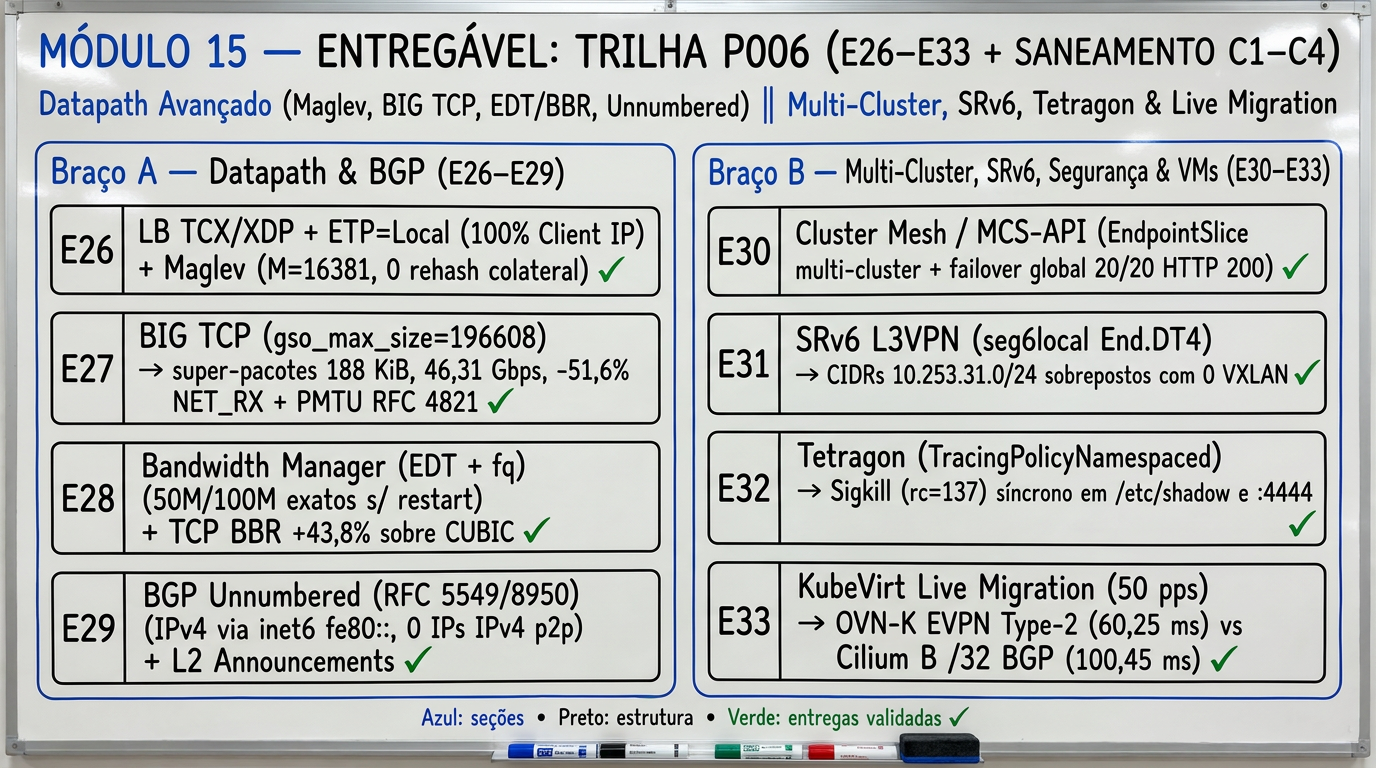
\includegraphics[width=\textwidth,height=0.72\textheight,keepaspectratio]{diagramas/m15-whiteboard-entregavel.png}
\fonte{elaborada pelo autor (2026).}
\end{figure}

\section{Onda 1 (P006-S001): LoadBalancer TCX/XDP com Maglev e Cluster Mesh}\label{onda-1-p006-s001-loadbalancer-tcxxdp-com-maglev-e-cluster-mesh}

Onda concluída com \textbf{PASS}; estudos \texttt{E26} e \texttt{E30} e saneamento do \texttt{Bloco C1}. O \texttt{E26} usa o hashing consistente Maglev (Eisenbud et al., 2016).

\textbf{Braço A --- LoadBalancer TCX/XDP, anúncio BGP seletivo e Maglev (\texttt{26-{}\allowbreak{}lb-{}\allowbreak{}xdp-{}\allowbreak{}dsr-{}\allowbreak{}maglev-{}\allowbreak{}clustermesh.\allowbreak{}md}):}

\begin{itemize}
\tightlist
\item
  \textbf{E26 --- anúncio seletivo e Maglev:} o estudo comparou três VIPs BGP, duas com \texttt{external\allowbreak{}Traffic\allowbreak{}Policy:\allowbreak{} Cluster} e uma com \texttt{external\allowbreak{}Traffic\allowbreak{}Policy:\allowbreak{} Local}. As VIPs \texttt{Cluster} foram anunciadas em ECMP pelos dois workers. A VIP \texttt{Local} foi anunciada só pelo worker que hospeda o backend, o que eliminou o salto intermediário e preservou 100\% (10/10) do IP real do cliente externo; nas VIPs \texttt{Cluster}, o nó aplicou SNAT. No anel Maglev (\texttt{M=\allowbreak{}16381}), a remoção de um backend realocou apenas os slots dele: houve 0 rehash colateral nos backends restantes, e o serviço respondeu 20/20 HTTP 200.
\end{itemize}

\textbf{Braço B --- Cluster Mesh e MCS-API com failover global sobre BGP (\texttt{26-{}\allowbreak{}lb-{}\allowbreak{}xdp-{}\allowbreak{}dsr-{}\allowbreak{}maglev-{}\allowbreak{}clustermesh.\allowbreak{}md}):}

\begin{itemize}
\tightlist
\item
  \textbf{E30 --- serviço global entre dois clusters:} o estudo uniu os clusters \texttt{k01} e \texttt{p003-{}\allowbreak{}gw}, cada um com identidade de cluster própria, e publicou um \texttt{Service} global. O Cilium mesclou os backends locais e remotos nos mapas eBPF de balanceamento. Com os dois clusters ativos, o serviço respondeu 20/20 no tráfego leste-oeste e 20/20 no norte-sul via BGP. Ao escalar o deployment local para 0, o failover global ocorreu sem perda: os mesmos 20/20 passaram a ser servidos pelo cluster remoto.
\item
  \textbf{E30 --- controles negativos:} uma \texttt{Cilium\allowbreak{}Network\allowbreak{}Policy} com \texttt{egress\allowbreak{}Deny} para o cluster remoto bloqueou 5/5 conexões (\texttt{3A}). Retirar a exportação dos backends remotos, com o local em 0, esvaziou o mapa BPF e recusou 5/5 conexões (\texttt{3B}).
\end{itemize}

\textbf{Braço C --- saneamento crítico do Bloco C1 (\texttt{revisao-{}\allowbreak{}projeto-{}\allowbreak{}2026-{}\allowbreak{}09-{}\allowbreak{}26.\allowbreak{}md}):}

\begin{itemize}
\tightlist
\item
  \textbf{Bloco C1:} os 8 itens críticos (\texttt{A4–A8}, \texttt{A10–A12}) foram resolvidos. A lista inclui erros de sintaxe Bash, a unificação de um documento duplicado, a remoção de chaves privadas estáticas e a leitura de senha a partir de arquivo de configuração.
\end{itemize}

\section{Onda 2 (P006-S002): BIG TCP com netkit e SRv6 L3VPN}\label{onda-2-p006-s002-big-tcp-com-netkit-e-srv6-l3vpn}

Onda concluída com \textbf{PASS}; estudos \texttt{E27} e \texttt{E31} e saneamento do \texttt{Bloco C2}. O \texttt{E27} recorre à descoberta de PMTU da RFC 4821 (Mathis; Heffner, 2007), e o \texttt{E31} usa o comportamento \texttt{End.\allowbreak{}DT4} do SRv6 (Filsfils et al., 2021).

\textbf{Braço A --- BIG TCP, \texttt{netkit} e MTU 9000 (\texttt{27-{}\allowbreak{}big-{}\allowbreak{}tcp-{}\allowbreak{}netkit-{}\allowbreak{}srv6-{}\allowbreak{}l3vpn.\allowbreak{}md}):}

\begin{itemize}
\tightlist
\item
  \textbf{E27 --- três regimes de datapath:} no Cilium \texttt{1.\allowbreak{}20.\allowbreak{}2} com kernel 6.8, o estudo comparou \texttt{veth} com MTU 1500 e GSO de 64k, \texttt{veth} com MTU 9000 e BIG TCP de 192k, e \texttt{netkit mode l3} com MTU 9000 e BIG TCP de 192k. Numa transferência TCP de fluxo único de 512 MiB, o throughput IPv4 subiu de 39,20 Gbps para 46,31 Gbps (+18,1\%) com \texttt{veth} e para 46,08 Gbps (+17,6\%) com \texttt{netkit}. Em IPv6, subiu de 41,61 Gbps para 46,60 Gbps (+12,0\%) e 45,73 Gbps (+9,9\%).
\item
  \textbf{E27 --- menos pacotes e menos interrupções:} os pacotes no fio caíram de -59,6\% a -60,8\%, e as interrupções \texttt{NET\_\allowbreak{}RX} caíram de -51,0\% a -51,6\%. O kernel gerou super-pacotes de até 187.974 B em IPv4 e 187.582 B em IPv6.
\item
  \textbf{E27 --- PMTU blackhole:} com MTU assimétrica (\texttt{9000 -{}\allowbreak{}\textgreater{} 1500 -{}\allowbreak{}\textgreater{} 9000}), a conexão convergiu enquanto o ICMP Frag-Needed chegava (5/5, \texttt{3A}). Com esse ICMP filtrado e \texttt{tcp\_\allowbreak{}mtu\_\allowbreak{}probing=\allowbreak{}0}, a conexão travou: 0/5 e timeout na transferência TCP (\texttt{3B}). Com \texttt{tcp\_\allowbreak{}mtu\_\allowbreak{}probing=\allowbreak{}2}, a descoberta de PMTU da RFC 4821 recuperou a transferência sem depender de ICMP (\texttt{3C}).
\end{itemize}

\textbf{Braço B --- SRv6 L3VPN sem VXLAN para sub-redes sobrepostas (\texttt{27-{}\allowbreak{}big-{}\allowbreak{}tcp-{}\allowbreak{}netkit-{}\allowbreak{}srv6-{}\allowbreak{}l3vpn.\allowbreak{}md}):}

\begin{itemize}
\tightlist
\item
  \textbf{E31 --- isolamento com \texttt{End.\allowbreak{}DT4}:} dois tenants usaram a mesma sub-rede \texttt{10.\allowbreak{}253.\allowbreak{}31.\allowbreak{}0/\allowbreak{}24} e os mesmos IPs, cada um na sua VRF. Ambos obtiveram 30/30 HTTP 200 dentro do próprio tenant, sem vazamento e com 0 interfaces VXLAN. A captura mostrou o cabeçalho SRH do SRv6 com um SID por tenant. O teste entre VRFs deu 0/5, e revogar o SID do Tenant B deu 0/5 para ele, enquanto o Tenant A manteve 5/5.
\item
  \textbf{E31 --- três exigências do kernel 6.8:} \texttt{net.\allowbreak{}vrf.\allowbreak{}strict\_\allowbreak{}mode=\allowbreak{}1} é obrigatório para criar \texttt{End.\allowbreak{}DT4}. A rota \texttt{seg6local} precisa indicar \texttt{dev eth0} para que o SID vá para a tabela \texttt{main}. Clientes na mesma \texttt{/\allowbreak{}24} lógica precisam de rota \texttt{/\allowbreak{}32} via gateway.
\end{itemize}

\textbf{Braço C --- saneamento de defaults e configurações do Bloco C2 (\texttt{revisao-{}\allowbreak{}projeto-{}\allowbreak{}2026-{}\allowbreak{}09-{}\allowbreak{}26.\allowbreak{}md}):}

\begin{itemize}
\tightlist
\item
  \textbf{Bloco C2:} os 10 itens (\texttt{A1–A3}, \texttt{A9}, \texttt{M1–M6}) foram concluídos. Os defaults dos scripts foram alinhados, a semântica de \texttt{ingress\allowbreak{}Deny}/\texttt{egress\allowbreak{}Deny} foi documentada, chaves inexistentes saíram dos values do Cilium 1.20 e alguns scripts ganharam detecção automática de interface, \texttt{-{}\allowbreak{}-{}\allowbreak{}dry-{}\allowbreak{}run} e versões fixadas.
\end{itemize}

\section{Onda 3 (P006-S003): Bandwidth Manager com BBR e Tetragon}\label{onda-3-p006-s003-bandwidth-manager-com-bbr-e-tetragon}

Onda concluída com \textbf{PASS}; estudos \texttt{E28} e \texttt{E32} e saneamento do \texttt{Bloco C3}. O \texttt{E28} compara o BBR (Cardwell et al., 2016) com o CUBIC (Xu et al., 2023), e o \texttt{E32} usa o Tetragon (Tetragon Authors, c2024).

\textbf{Braço A --- Bandwidth Manager, pacing por pod e BBR versus CUBIC (\texttt{28-{}\allowbreak{}bandwidth-{}\allowbreak{}edt-{}\allowbreak{}bbr-{}\allowbreak{}tetragon.\allowbreak{}md}):}

\begin{itemize}
\tightlist
\item
  \textbf{E28 --- limite de banda por pod:} no Cilium \texttt{1.\allowbreak{}20.\allowbreak{}2}, o estudo ativou o Bandwidth Manager com \texttt{qdisc fq}. Para isso, foi preciso remontar \texttt{/\allowbreak{}proc/\allowbreak{}sys} como \texttt{rw}, porque os contêineres do \texttt{kind} o montam como \texttt{ro}. A anotação \texttt{kubernetes.\allowbreak{}io/\allowbreak{}egress-{}\allowbreak{}bandwidth} limitou o pod a \texttt{49,\allowbreak{}70 Mbps} e \texttt{49,\allowbreak{}62 Mbps} com teto de \texttt{50M} (\texttt{99,\allowbreak{}2\%–99,\allowbreak{}4\%} de precisão) e a \texttt{97,\allowbreak{}34 Mbps} e \texttt{97,\allowbreak{}70 Mbps} com teto de \texttt{100M} (\texttt{97,\allowbreak{}3\%–97,\allowbreak{}7\%}). Sem limite, o pod alcançou 8,49 Gbps e 8,94 Gbps.
\item
  \textbf{E28 --- remoção dinâmica:} retirar a anotação de \texttt{50M} restaurou 8,40 Gbps e 9,00 Gbps sem reiniciar o pod. Uma anotação inválida não derrubou o \texttt{cilium-{}\allowbreak{}agent}.
\item
  \textbf{E28 --- BBR versus CUBIC:} num enlace WAN degradado (\texttt{delay 10ms loss 0.\allowbreak{}5\% rate 500mbit}), o BBR superou o CUBIC em +37,5\% (\texttt{163,\allowbreak{}20 Mbps} contra \texttt{118,\allowbreak{}71 Mbps}) e em +43,8\% (\texttt{237,\allowbreak{}36 Mbps} contra \texttt{165,\allowbreak{}01 Mbps}).
\end{itemize}

\textbf{Braço B --- Tetragon: observação e bloqueio em tempo de execução (\texttt{28-{}\allowbreak{}bandwidth-{}\allowbreak{}edt-{}\allowbreak{}bbr-{}\allowbreak{}tetragon.\allowbreak{}md}):}

\begin{itemize}
\tightlist
\item
  \textbf{E32 --- política \texttt{Tracing\allowbreak{}Policy\allowbreak{}Namespaced}:} a política, aplicada a um namespace, correlacionou execuções de processo, leituras de arquivos críticos e conexões de saída com o pod e com a identidade Cilium. As tentativas de ler \texttt{/\allowbreak{}etc/\allowbreak{}shadow} e de abrir conexão para a porta 4444 foram encerradas na hora com \texttt{SIGKILL} (\texttt{rc=\allowbreak{}137}), com 0 bytes vazados. O tráfego HTTP legítimo completou 10/10 (100\%) \texttt{HTTP 200 OK}.
\end{itemize}

\textbf{Braço C --- saneamento dos scripts P003 e das fixtures Go/Docker do Bloco C3 (\texttt{revisao-{}\allowbreak{}projeto-{}\allowbreak{}2026-{}\allowbreak{}09-{}\allowbreak{}26.\allowbreak{}md}):}

\begin{itemize}
\tightlist
\item
  \textbf{Bloco C3:} os 9 itens (\texttt{M7–M15}) foram concluídos. Entre eles estão guardas de segurança em scripts do testbed, um contêiner DevStack válido, a fixture de autorização com \texttt{go test .\allowbreak{}/\allowbreak{}.\allowbreak{}.\allowbreak{}.\allowbreak{}} PASS, o código-fonte da fixture TLS, a limpeza de referências privadas e a documentação do \texttt{k8s\allowbreak{}Service\allowbreak{}Host} dinâmico.
\end{itemize}

\section{Onda 4 (P006-S004): BGP unnumbered, L2 Announcements e live migration}\label{onda-4-p006-s004-bgp-unnumbered-l2-announcements-e-live-migration}

Onda concluída com \textbf{PASS} na versão \texttt{v2.\allowbreak{}5.\allowbreak{}0}; estudos \texttt{E29} e \texttt{E33} e saneamento final do \texttt{Bloco C4}. O \texttt{E29} aplica o next hop IPv6 para NLRI IPv4 definido na RFC 5549 e na RFC 8950 (Le Faucheur; Rosen, 2009; Litkowski et al., 2020).

\textbf{Braço A --- BGP unnumbered e L2 Announcements (\texttt{29-{}\allowbreak{}bgp-{}\allowbreak{}unnumbered-{}\allowbreak{}l2-{}\allowbreak{}live-{}\allowbreak{}migration.\allowbreak{}md}):}

\begin{itemize}
\tightlist
\item
  \textbf{E29 --- eBGP unnumbered:} a sessão eBGP entre o ToR e o nó usou apenas endereços IPv6 link-local, com 0 endereços IPv4 nas interfaces ponto a ponto. Mesmo assim, o kernel instalou as rotas IPv4 com próximo salto IPv6 (\texttt{via inet6 fe80:\allowbreak{}:\allowbreak{}.\allowbreak{}.\allowbreak{}.\allowbreak{}}) e respondeu 10/10 pings, com \texttt{RTT avg =\allowbreak{} 0,\allowbreak{}060 ms}.
\item
  \textbf{E29 --- L2 Announcements:} com \texttt{enable-{}\allowbreak{}l2-{}\allowbreak{}announcements=\allowbreak{}true} no Cilium \texttt{1.\allowbreak{}20.\allowbreak{}2}, um nó venceu a eleição de líder pelo objeto \texttt{Lease}. O Cilium programou o mapa \texttt{cilium\_\allowbreak{}l2\_\allowbreak{}responder\_\allowbreak{}v4} e o segmento L2 obteve 10/10 HTTP 200.
\item
  \textbf{E29 --- controles negativos:} desativar a família IPv4 retirou a rota da FIB. Remover a label do Service esvaziou na hora o \texttt{cilium\_\allowbreak{}l2\_\allowbreak{}responder\_\allowbreak{}v4}.
\end{itemize}

\textbf{Braço B --- live migration de VM KubeVirt sob tráfego contínuo (\texttt{29-{}\allowbreak{}bgp-{}\allowbreak{}unnumbered-{}\allowbreak{}l2-{}\allowbreak{}live-{}\allowbreak{}migration.\allowbreak{}md}):}

\begin{itemize}
\tightlist
\item
  \textbf{E33 --- método:} o estudo enviou à VM um fluxo contínuo de 50 pps (20 ms entre pacotes, 150 pacotes UDP numerados por ensaio) durante a migração entre dois workers.
\item
  \textbf{E33 --- Cilium B com \texttt{/\allowbreak{}32} por BGP:} a troca de rota perdeu 5/150 pacotes (3,3\%), com blackout de 100,45 ms.
\item
  \textbf{E33 --- OVN-Kubernetes com EVPN:} preservando MAC e IP e atualizando o FDB VXLAN, a migração perdeu 3/150 pacotes (2,0\%), com blackout de 60,25 ms, uma janela -40,0\% menor.
\item
  \textbf{E33 --- controle negativo:} manter a rota \texttt{/\allowbreak{}32} apontando para o nó de origem após a migração entregou 0/10 pacotes (100\% blackhole); a atualização BGP restaurou 10/10 na hora.
\end{itemize}

\textbf{Braço C --- higiene contínua e fechamento do Bloco C4 (\texttt{revisao-{}\allowbreak{}projeto-{}\allowbreak{}2026-{}\allowbreak{}09-{}\allowbreak{}26.\allowbreak{}md}):}

\begin{itemize}
\tightlist
\item
  \textbf{Bloco C4:} os itens restantes da revisão foram resolvidos (100\%). Os \texttt{Makefile} e \texttt{poc-{}\allowbreak{}k8s-{}\allowbreak{}fabric/\allowbreak{}Makefile} ganharam \texttt{make lint} (204/204 scripts \texttt{.\allowbreak{}sh} sem erro, 0 chaves privadas, \texttt{go vet} OK), \texttt{make test} (\texttt{go test} 4/4 PASS e 23/23 scripts \texttt{-{}\allowbreak{}-{}\allowbreak{}dry-{}\allowbreak{}run} PASS) e \texttt{make pdf}. Também foram criados os índices \texttt{studies/\allowbreak{}p003/\allowbreak{}cases/\allowbreak{}s011/\allowbreak{}README.\allowbreak{}md} e \texttt{studies/\allowbreak{}p003/\allowbreak{}cases/\allowbreak{}s012/\allowbreak{}README.\allowbreak{}md} e atualizado o \texttt{student-{}\allowbreak{}guide-{}\allowbreak{}template.\allowbreak{}md}.
\end{itemize}

\section{Exercícios de interpretação}\label{exercuxedcios-de-interpretauxe7uxe3o-2}

\begin{enumerate}
\def\labelenumi{\arabic{enumi}.}
\tightlist
\item
  No estudo \texttt{E26}, por que a VIP \texttt{10.\allowbreak{}202.\allowbreak{}255.\allowbreak{}28/\allowbreak{}32} (\texttt{external\allowbreak{}Traffic\allowbreak{}Policy:\allowbreak{} Local}) é anunciada por BGP apenas por \texttt{p003-{}\allowbreak{}gw-{}\allowbreak{}worker2} (\texttt{AS 65302}) e preserva 100\% do IP de origem do cliente (\texttt{198.\allowbreak{}19.\allowbreak{}0.\allowbreak{}10}), e como o anel primo \textbf{Maglev (\texttt{M=\allowbreak{}16381})} evita rehash colateral (0 diffs nos backends sobreviventes) quando um backend sai do pool?
\item
  No estudo \texttt{E27} (\textbf{BIG TCP} + \texttt{netkit}) e no estudo \texttt{E31} (\textbf{SRv6 \texttt{End.\allowbreak{}DT4}}), por que bloquear \texttt{ICMP Type 3 Code 4} derruba conexões TCP grandes sob \texttt{tcp\_\allowbreak{}mtu\_\allowbreak{}probing=\allowbreak{}0} mas é contornado automaticamente por \texttt{tcp\_\allowbreak{}mtu\_\allowbreak{}probing=\allowbreak{}2} (\texttt{RFC 4821}), e por que o kernel Linux 6.8 exige \texttt{net.\allowbreak{}vrf.\allowbreak{}strict\_\allowbreak{}mode=\allowbreak{}1} e \texttt{dev eth0} explícito ao instalar rotas locais \texttt{seg6local action End.\allowbreak{}DT4}?
\item
  No estudo \texttt{E28} (\textbf{Bandwidth Manager EDT}) e no estudo \texttt{E32} (\textbf{Tetragon}), como a remoção dinâmica da anotação \texttt{kubernetes.\allowbreak{}io/\allowbreak{}egress-{}\allowbreak{}bandwidth} restaura a vazão de \texttt{49,\allowbreak{}7 Mbps} para \texttt{\textasciitilde{}9 Gbps} sem reiniciar o pod, e qual a diferença entre bloquear conexões no datapath L3/L4 (\texttt{Cilium\allowbreak{}Network\allowbreak{}Policy}) versus terminar sincronicamente o processo infrator (\texttt{Sigkill} \texttt{rc=\allowbreak{}137}) no hook LSM/kprobe (\texttt{security\_\allowbreak{}file\_\allowbreak{}permission} / \texttt{tcp\_\allowbreak{}connect})?
\item
  No estudo \texttt{E29} (\textbf{BGP Unnumbered \texttt{RFC 5549}/8950} + \textbf{L2 Announcements}), como o kernel Linux resolve o endereço MAC de próximo salto para um pacote IPv4 cuja rota aponta para \texttt{via inet6 fe80:\allowbreak{}:\allowbreak{}.\allowbreak{}.\allowbreak{}.\allowbreak{}} em uma interface sem endereço IPv4, e qual é o papel do objeto \texttt{Lease/\allowbreak{}cilium-{}\allowbreak{}l2announce-{}\allowbreak{}*} e do mapa BPF \texttt{cilium\_\allowbreak{}l2\_\allowbreak{}responder\_\allowbreak{}v4}?
\item
  No estudo \texttt{E33} (\textbf{KubeVirt Live Migration sob Tráfego Contínuo}), por que a migração com \textbf{OVN-Kubernetes EVPN Type-2 (\texttt{VNI 10033})} apresentou menor tempo de blackout (60,25 ms, 3 pacotes perdidos) e preservou conexões L2 em comparação ao cutover \textbf{Cilium B L3 \texttt{/\allowbreak{}32} BGP} (100,45 ms, 5 pacotes perdidos), e o que ocorre (0/10) se o anúncio \texttt{/\allowbreak{}32} não acompanhar a VM migrada?
\end{enumerate}

\chapter{Trilha P007: BGP sem perda, SPIFFE com WireGuard, Local Redirect e Multus}\label{trilha-p007-bgp-sem-perda-spiffe-com-wireguard-local-redirect-e-multus}

A trilha P007 encerra a Fase 3 em duas ondas. O Braço A trata da operação BGP
sem perda de pacotes e do roteamento local ao nó (\texttt{E34} e \texttt{E36}); o Braço B, de
segurança zero-trust com SPIFFE e WireGuard e de workloads com duas interfaces
via Multus (\texttt{E35} e \texttt{E37}). Com ela, na versão \texttt{v2.\allowbreak{}6.\allowbreak{}0}, o projeto chegou a 37
estudos. A Figura 21 sintetiza o entregável do módulo.

\begin{figure}[!htbp]
\caption{Síntese visual do entregável do Módulo 16: Trilha P007 (E34--E37 --- BGP
Graceful Shutdown Zero-Loss, SPIFFE mTLS + WireGuard, Local Redirect
eBPF e Multus ipvlan L2/L3)}
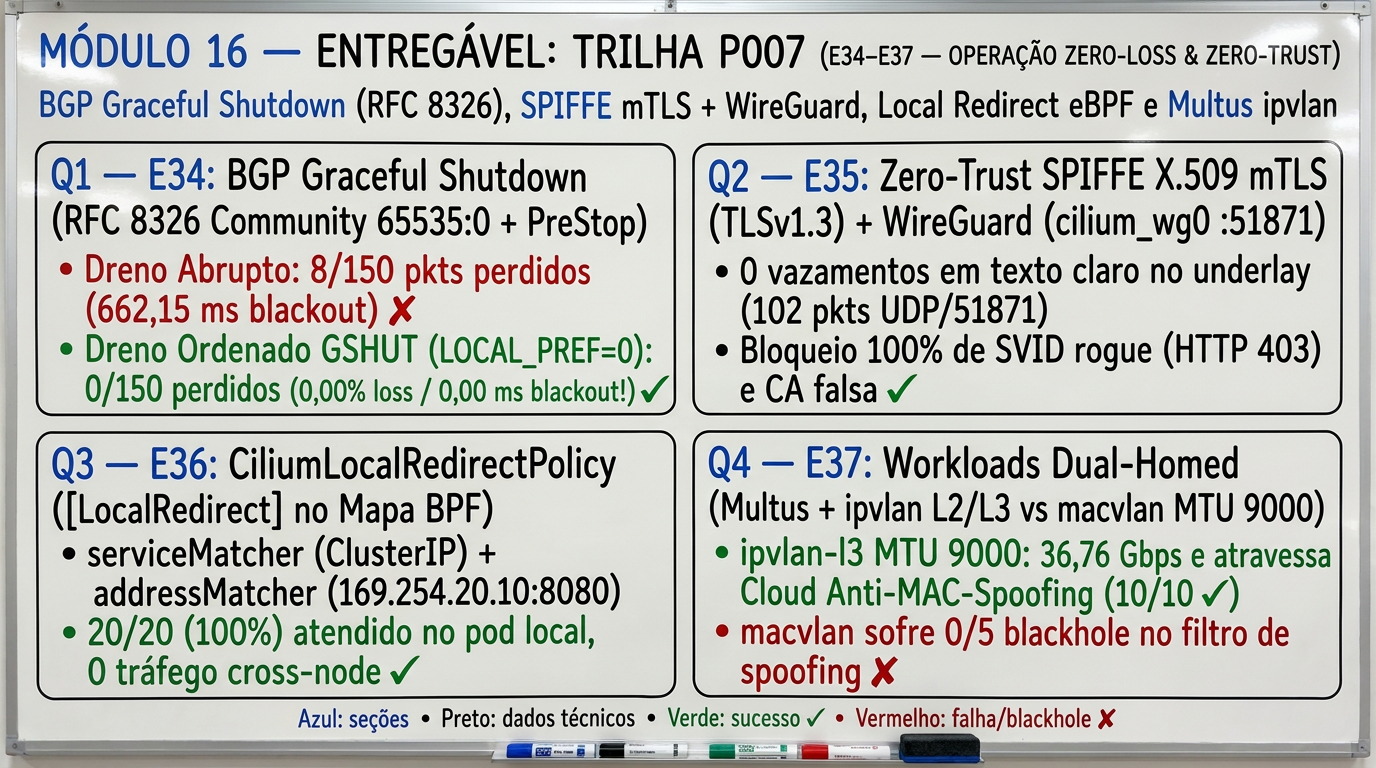
\includegraphics[width=\textwidth,height=0.72\textheight,keepaspectratio]{diagramas/m16-whiteboard-entregavel.png}
\fonte{elaborada pelo autor (2026).}
\end{figure}

\section{Onda 1 (P007-S001): BGP Graceful Shutdown e autenticação mútua SPIFFE}\label{onda-1-p007-s001-bgp-graceful-shutdown-e-autenticauxe7uxe3o-muxfatua-spiffe}

Onda concluída com \textbf{PASS}; estudos \texttt{E34} e \texttt{E35}. O \texttt{E34} aplica a RFC 8326 (Francois et al., 2018), e o \texttt{E35} combina identidades SPIFFE (SPIFFE, {[}2026{]}) com o WireGuard (Donenfeld, 2017).

\begin{itemize}
\tightlist
\item
  \textbf{Braço A --- BGP Graceful Shutdown e dreno de nó sem perda (\texttt{30-{}\allowbreak{}bgp-{}\allowbreak{}gshut-{}\allowbreak{}spiffe-{}\allowbreak{}mtls-{}\allowbreak{}wireguard.\allowbreak{}md}):}

  \begin{itemize}
  \tightlist
  \item
    \textbf{E34 --- dreno sem perda com GSHUT:} dois nós anunciaram a mesma VIP anycast a um ToR, em ECMP. O ToR rebaixa para \texttt{LOCAL\_\allowbreak{}PREF=\allowbreak{}0} qualquer rota marcada com a community well-known \texttt{graceful-{}\allowbreak{}shutdown} (\texttt{65535:\allowbreak{}0}). Sob fluxo contínuo de 50 pps (150 pacotes numerados), o dreno abrupto, que encerra o backend antes de retirar a rota, perdeu 8/150 pacotes (5,33\%) com 662,15 ms de blackout. O dreno ordenado anuncia \texttt{65535:\allowbreak{}0} e mantém o pod vivo em \texttt{Pre\allowbreak{}Stop} por 0,80 s; o ToR desviou 100\% dos novos pacotes para o outro nó e a perda caiu para 0/150 (0,00 ms de blackout).
  \item
    \textbf{E34 --- GSHUT declarativo no Cilium:} no Cilium \texttt{1.\allowbreak{}20.\allowbreak{}2}, um \texttt{Cilium\allowbreak{}BGPAdvertisement} injetou a community \texttt{65535:\allowbreak{}0} e \texttt{local\allowbreak{}Preference:\allowbreak{} 0} na VIP sem configuração manual no roteador.
  \item
    \textbf{E34 --- controles:} uma rota em GSHUT ainda encaminhou 10/10 pacotes como último recurso quando não havia alternativa (\texttt{3A}). Ela caiu para 0/5 quando os dois nós retiraram a rota (\texttt{3B}) e voltou a 10/10 em ECMP ao remover \texttt{65535:\allowbreak{}0} (\texttt{3C}, \texttt{R6=\allowbreak{}0}).
  \end{itemize}
\item
  \textbf{Braço B --- autenticação mútua SPIFFE com criptografia WireGuard (\texttt{30-{}\allowbreak{}bgp-{}\allowbreak{}gshut-{}\allowbreak{}spiffe-{}\allowbreak{}mtls-{}\allowbreak{}wireguard.\allowbreak{}md}):}

  \begin{itemize}
  \tightlist
  \item
    \textbf{E35 --- WireGuard entre nós:} sem túnel, o \texttt{tcpdump} no underlay leu 20 pacotes HTTP em texto claro. Com \texttt{cilium\_\allowbreak{}wg0} (\texttt{UDP :\allowbreak{}51871}), o serviço respondeu 10/10 HTTP 200; a captura mostrou 102 pacotes UDP cifrados e 0 vazamentos em texto claro.
  \item
    \textbf{E35 --- mTLS com identidade SPIFFE:} uma CA SPIFFE emitiu certificados X.509 SVID para cliente e servidor. A \texttt{Cilium\allowbreak{}Network\allowbreak{}Policy} exigiu autenticação (\texttt{authentication.\allowbreak{}mode:\allowbreak{} "required"}). O servidor respondeu 10/10 HTTP 200 com autenticação mútua em \texttt{TLSv1.\allowbreak{}3}.
  \item
    \textbf{E35 --- controles:} o Cilium bloqueou 100\% das tentativas em três casos. Um SVID válido com SPIFFE ID não autorizado recebeu 5/5 HTTP 403 (\texttt{3A}). Um SVID assinado por CA externa falhou no handshake com \texttt{SSLV3\_\allowbreak{}ALERT\_\allowbreak{}BAD\_\allowbreak{}CERTIFICATE} (0/5, \texttt{3B}). Uma regra \texttt{ingress\allowbreak{}Deny} bloqueou 0/5 (\texttt{3C}), e o acesso voltou a 10/10 ao remover a regra (\texttt{R6=\allowbreak{}0}).
  \end{itemize}
\end{itemize}

\section{Onda 2 (P007-S002): Local Redirect Policy e workloads dual-homed com Multus}\label{onda-2-p007-s002-local-redirect-policy-e-workloads-dual-homed-com-multus}

Onda concluída com \textbf{PASS} na versão \texttt{v2.\allowbreak{}6.\allowbreak{}0}; estudos \texttt{E36} e \texttt{E37}.

\begin{itemize}
\tightlist
\item
  \textbf{Braço A --- Local Redirect Policy e atalho local no datapath eBPF (\texttt{31-{}\allowbreak{}local-{}\allowbreak{}redirect-{}\allowbreak{}multus-{}\allowbreak{}ipvlan-{}\allowbreak{}dualhomed.\allowbreak{}md}):}

  \begin{itemize}
  \tightlist
  \item
    \textbf{E36 --- redirecionar um Service para o pod do próprio nó:} sem a política, chamadas ao \texttt{Cluster\allowbreak{}IP} de um cache em \texttt{Daemon\allowbreak{}Set} cruzaram para o outro nó em \textasciitilde40\%--60\% das vezes. Com uma \texttt{Cilium\allowbreak{}Local\allowbreak{}Redirect\allowbreak{}Policy} de \texttt{service\allowbreak{}Matcher}, cada \texttt{cilium-{}\allowbreak{}agent} marcou a entrada do Service no mapa BPF como \texttt{[Local\allowbreak{}Redirect]}. 100\% (20/20) das requisições ficaram no próprio nó, com 0 pacotes entre nós.
  \item
    \textbf{E36 --- redirecionar um endereço sem Service:} com \texttt{address\allowbreak{}Matcher}, o endereço link-local \texttt{169.\allowbreak{}254.\allowbreak{}20.\allowbreak{}10:\allowbreak{}8080/\allowbreak{}TCP} foi entregue ao pod local em 10/10 conexões em cada nó.
  \item
    \textbf{E36 --- controles:} tirar a label de seleção de um nó afetou só esse nó (0/5), e o outro manteve 10/10 (\texttt{3A}). Apagar as duas políticas limpou 100\% das entradas \texttt{[Local\allowbreak{}Redirect]}, com 0 resíduos, e o balanceamento normal voltou (20/20, \texttt{3B}, \texttt{R6=\allowbreak{}0}).
  \end{itemize}
\item
  \textbf{Braço B --- workloads dual-homed com Multus, \texttt{ipvlan} e \texttt{macvlan} (\texttt{31-{}\allowbreak{}local-{}\allowbreak{}redirect-{}\allowbreak{}multus-{}\allowbreak{}ipvlan-{}\allowbreak{}dualhomed.\allowbreak{}md}):}

  \begin{itemize}
  \tightlist
  \item
    \textbf{E37 --- duas interfaces no mesmo pod:} um \texttt{Network\allowbreak{}Attachment\allowbreak{}Definition} deu aos pods uma segunda interface \texttt{net1} (\texttt{ipvlan mode l2}, \texttt{MTU 9000}) ao lado da \texttt{eth0} do Cilium. A \texttt{eth0} continuou protegida por \texttt{Cilium\allowbreak{}Network\allowbreak{}Policy} e respondeu 10/10 HTTP 200. A \texttt{net1} respondeu 10/10 HTTP 200 e 10/10 pings Jumbo de 8972 B com \texttt{DF=\allowbreak{}1}, 0\% de perda e \texttt{RTT avg =\allowbreak{} 0,\allowbreak{}069 ms}.
  \item
    \textbf{E37 --- desempenho:} num fluxo TCP único de 512 MiB, o \texttt{veth 1500} atingiu 33,01 Gbps, o \texttt{macvlan} 32,49 Gbps e o \texttt{ipvlan l2} 30,63 Gbps. O \texttt{ipvlan l3} (\texttt{NOARP}) foi o mais rápido: 36,76 Gbps, +11,4\% sobre o \texttt{veth 1500} e +20,0\% sobre o \texttt{ipvlan l2}.
  \item
    \textbf{E37 --- antispoofing de nuvem:} um filtro que só aceita o MAC da NIC do host imitou a porta de uma nuvem pública. O \texttt{macvlan} usa MAC próprio e perdeu 100\% dos pacotes (0/5); o \texttt{ipvlan mode l2} reaproveita o MAC do host e passou 10/10 (\texttt{3A}). Derrubar a \texttt{net1} não afetou a \texttt{eth0}, que manteve 10/10 (\texttt{3B}, \texttt{R6=\allowbreak{}0}).
  \end{itemize}
\end{itemize}

\section{Exercícios de interpretação}\label{exercuxedcios-de-interpretauxe7uxe3o-3}

\begin{enumerate}
\def\labelenumi{\arabic{enumi}.}
\tightlist
\item
  No estudo \texttt{E34} (\textbf{BGP Graceful Shutdown \texttt{RFC 8326}}), por que anunciar a community well-known \texttt{65535:\allowbreak{}0} (\texttt{GSHUT}, \texttt{LOCAL\_\allowbreak{}PREF=\allowbreak{}0}) antes de iniciar o término do pod reduz a perda de pacotes de 8/150 (662,15 ms de blackout no dreno abrupto) para \textbf{0/150 (0,00 ms)}, e por que manter a rota com \texttt{LOCAL\_\allowbreak{}PREF=\allowbreak{}0} é mais seguro do que retirá-la imediatamente se o segundo nó também falhar (\texttt{3A} vs \texttt{3B})?
\item
  No estudo \texttt{E35} (\textbf{Cilium Mutual Auth SPIFFE + WireGuard}), quais ameaças distintas são mitigadas pelo túnel L3 \texttt{cilium\_\allowbreak{}wg0} (\texttt{UDP :\allowbreak{}51871}) versus o handshake mTLS com SVID X.509 (\texttt{spiffe:\allowbreak{}/\allowbreak{}/\allowbreak{}spiffe.\allowbreak{}cilium/\allowbreak{}ns/\allowbreak{}.\allowbreak{}.\allowbreak{}.\allowbreak{}/\allowbreak{}sa/\allowbreak{}.\allowbreak{}.\allowbreak{}.\allowbreak{}}), e por que um pod com certificado criptograficamente válido assinado pela mesma CA \texttt{spiffe.\allowbreak{}cilium} ainda recebe \texttt{HTTP 403} no controle \texttt{3A} (\texttt{e35-{}\allowbreak{}client-{}\allowbreak{}rogue})?
\item
  No estudo \texttt{E36} (\textbf{\texttt{Cilium\allowbreak{}Local\allowbreak{}Redirect\allowbreak{}Policy}}), qual é a diferença operacional entre usar \texttt{service\allowbreak{}Matcher} (sobrescrevendo um \texttt{Cluster\allowbreak{}IP} existente com \texttt{[Local\allowbreak{}Redirect]} no mapa BPF de cada nó) e \texttt{address\allowbreak{}Matcher} (interceptando um IP link-local como \texttt{169.\allowbreak{}254.\allowbreak{}20.\allowbreak{}10:\allowbreak{}8080/\allowbreak{}TCP} sem criar \texttt{Service}), e o que acontece em um nó específico se o pod local de cache deixar de rodar nele (\texttt{3A})?
\item
  No estudo \texttt{E37} (\textbf{Multus + \texttt{ipvlan L2/\allowbreak{}L3} vs \texttt{macvlan}}), por que switches de nuvem pública (VPC / SDN com \emph{Port-Security} / \emph{MAC Anti-Spoofing}) bloqueiam pacotes de interfaces \texttt{macvlan} (0/5 no controle \texttt{3A}) mas permitem \texttt{ipvlan mode l2/\allowbreak{}l3} (10/10), e por que o \texttt{ipvlan mode l3} (\texttt{NOARP}, \texttt{MTU 9000}) atingiu o maior throughput (36,76 Gbps, +11,4\% sobre \texttt{veth 1500})?
\end{enumerate}

\chapter{Trilha P008: Host Firewall, CiliumEnvoyConfig, Route Reflector e matriz netkit}\label{trilha-p008-host-firewall-ciliumenvoyconfig-route-reflector-e-matriz-netkit}

A trilha P008 encerra a Fase 4 em duas ondas. O Braço A protege o nó com Host
Firewall e XDP e escala o BGP com Route Reflector e SRv6 dual-stack (\texttt{E38} e
\texttt{E40}); o Braço B trata de resiliência L7 com \texttt{Cilium\allowbreak{}Envoy\allowbreak{}Config} e mede a
combinação de \texttt{netkit}, BIG TCP e WireGuard (\texttt{E39} e \texttt{E41}). Com ela, na versão
\texttt{v2.\allowbreak{}7.\allowbreak{}0}, o projeto completou os 41 estudos (\texttt{E01}--\texttt{E41}). A Figura 22 sintetiza o entregável do módulo.

\begin{figure}[!htbp]
\caption{Síntese visual do entregável do Módulo 17: Trilha P008 (E38--E41 ---
Host Firewall + XDP\_DROP, CiliumEnvoyConfig L7, iBGP RR + SRv6
Dual-Stack e Matriz netkit + BIG TCP + WireGuard 5,59x)}
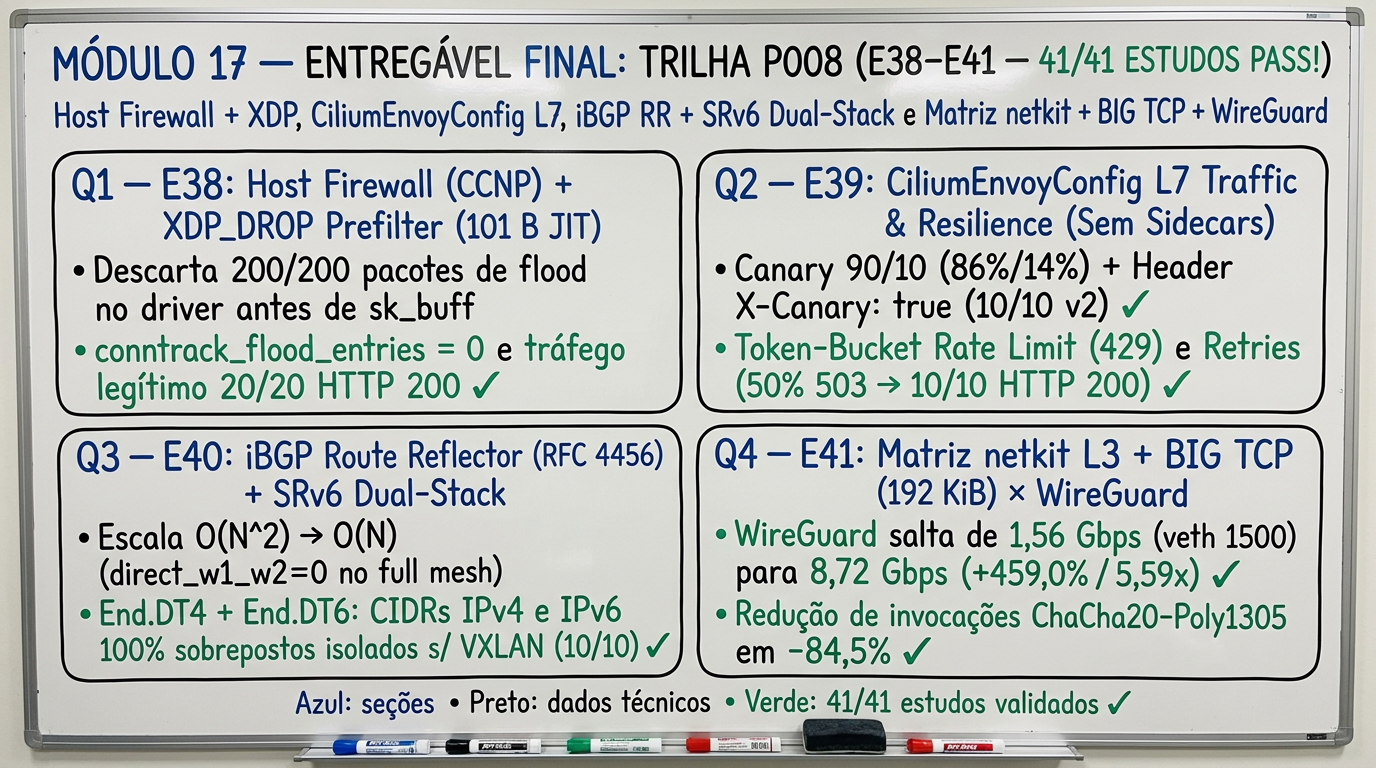
\includegraphics[width=\textwidth,height=0.72\textheight,keepaspectratio]{diagramas/m17-whiteboard-entregavel.png}
\fonte{elaborada pelo autor (2026).}
\end{figure}

\section{Onda 1 (P008-S001): Host Firewall com XDP e resiliência L7 com CiliumEnvoyConfig}\label{onda-1-p008-s001-host-firewall-com-xdp-e-resiliuxeancia-l7-com-ciliumenvoyconfig}

Onda concluída com \textbf{PASS}; estudos \texttt{E38} e \texttt{E39}.

\begin{itemize}
\tightlist
\item
  \textbf{Braço A --- Host Firewall e prefiltro XDP no nó (\texttt{32-{}\allowbreak{}host-{}\allowbreak{}firewall-{}\allowbreak{}xdp-{}\allowbreak{}envoy-{}\allowbreak{}l7-{}\allowbreak{}resilience.\allowbreak{}md}):}

  \begin{itemize}
  \tightlist
  \item
    \textbf{E38 --- Host Firewall e descarte antecipado com XDP:} o estudo ativou \texttt{enable-{}\allowbreak{}host-{}\allowbreak{}firewall=\allowbreak{}true} no Cilium \texttt{1.\allowbreak{}20.\allowbreak{}2} e aplicou uma \texttt{Cilium\allowbreak{}Clusterwide\allowbreak{}Network\allowbreak{}Policy} com \texttt{node\allowbreak{}Selector} para proteger as portas do host (\texttt{:\allowbreak{}10250}, \texttt{:\allowbreak{}6443}, \texttt{:\allowbreak{}4240}, \texttt{:\allowbreak{}179}, \texttt{:\allowbreak{}19100}). Sem a política, tanto o cliente administrativo quanto um host não autorizado alcançaram a porta \texttt{:\allowbreak{}19100} (10/10 cada). Com o Host Firewall ativo, o cliente administrativo e o kubelet em \texttt{:\allowbreak{}10250} mantiveram 10/10 HTTP 200, e o host não autorizado caiu para 0/5 (\texttt{tc\_\allowbreak{}host\_\allowbreak{}fw\_\allowbreak{}drops=\allowbreak{}5}). Em seguida, um programa \texttt{BPF\_\allowbreak{}PROG\_\allowbreak{}TYPE\_\allowbreak{}XDP} de 101 B JIT, anexado no driver, descartou 200/200 (100\%) dos pacotes de um flood UDP em \texttt{XDP\_\allowbreak{}DROP}, antes da alocação de \texttt{sk\_\allowbreak{}buff}. O flood não criou entradas de conntrack (\texttt{conntrack\_\allowbreak{}flood\_\allowbreak{}entries=\allowbreak{}0}), e o cliente legítimo recebeu 20/20 HTTP 200. Os controles confirmaram que, sem o XDP, o bloqueio passa à segunda camada (TC Host Firewall, 0/5 entregues), que os nós dos dois clusters seguiram \texttt{Ready} (3/3 em cada) e que o rollback restaurou 10/10 com \texttt{R6=\allowbreak{}0}.
  \end{itemize}
\item
  \textbf{Braço B --- gestão de tráfego L7 com \texttt{Cilium\allowbreak{}Envoy\allowbreak{}Config} (\texttt{32-{}\allowbreak{}host-{}\allowbreak{}firewall-{}\allowbreak{}xdp-{}\allowbreak{}envoy-{}\allowbreak{}l7-{}\allowbreak{}resilience.\allowbreak{}md}):}

  \begin{itemize}
  \tightlist
  \item
    \textbf{E39 --- canário, roteamento por cabeçalho, limite de taxa e retries no Envoy:} o estudo registrou uma \texttt{Cilium\allowbreak{}Envoy\allowbreak{}Config} no \texttt{cilium-{}\allowbreak{}envoy 1.\allowbreak{}37.\allowbreak{}6}, sem sidecars, na frente de um Service. No canário ponderado 90/10, 100 requisições foram para \texttt{v1=\allowbreak{}86} e \texttt{v2=\allowbreak{}14}, todas com HTTP 200. Com o cabeçalho \texttt{X-{}\allowbreak{}Canary:\allowbreak{} true}, 10/10 chamadas foram para a versão \texttt{v2}. O limite de taxa por token bucket (\texttt{max\_\allowbreak{}tokens:\allowbreak{} 5}) deixou passar 5/15 requisições e devolveu 10/15 HTTP \texttt{429 Too Many Requests}; as excedentes pararam no Envoy do nó, sem chegar à aplicação. Contra um upstream que falha 50\% das vezes com HTTP 503, a rota sem retry entregou 5/10 HTTP 200, e a rota com \texttt{retry\_\allowbreak{}policy} (\texttt{retry\_\allowbreak{}on:\allowbreak{} 5xx}, \texttt{num\_\allowbreak{}retries:\allowbreak{} 3}) entregou 10/10 HTTP 200.
  \end{itemize}
\end{itemize}

\section{Onda 2 (P008-S002): Route Reflector com SRv6 dual-stack e matriz netkit, BIG TCP e WireGuard}\label{onda-2-p008-s002-route-reflector-com-srv6-dual-stack-e-matriz-netkit-big-tcp-e-wireguard}

Onda concluída com \textbf{PASS} na versão \texttt{v2.\allowbreak{}7.\allowbreak{}0}; estudos \texttt{E40} e \texttt{E41}. O \texttt{E40} aplica a reflexão de rotas da RFC 4456 (Bates; Chen; Chandra, 2006) e os comportamentos \texttt{End.\allowbreak{}DT4} e \texttt{End.\allowbreak{}DT6} do SRv6 (Filsfils et al., 2021).

\begin{itemize}
\tightlist
\item
  \textbf{Braço A --- Route Reflector iBGP e SRv6 dual-stack (\texttt{33-{}\allowbreak{}bgp-{}\allowbreak{}rr-{}\allowbreak{}srv6-{}\allowbreak{}dualstack-{}\allowbreak{}netkit-{}\allowbreak{}wg-{}\allowbreak{}matrix.\allowbreak{}md}):}

  \begin{itemize}
  \tightlist
  \item
    \textbf{E40 --- Route Reflector e VPN L3 SRv6 IPv4 e IPv6:} o estudo trocou a malha completa de sessões iBGP (\texttt{O(\allowbreak{}N\textasciicircum{}2)}) por um Route Reflector (\texttt{O(\allowbreak{}N)}), sem nenhuma sessão direta entre os workers (\texttt{direct\_\allowbreak{}w1\_\allowbreak{}w2=\allowbreak{}0}). O refletor repassou as VIPs IPv4 e IPv6, preservou o next hop do worker que as anunciou e marcou as rotas com os atributos anti-loop \texttt{Originator} e \texttt{Cluster list}; o tráfego direto entre os workers passou 10/10 em IPv4 e 10/10 em IPv6. Depois, o plano SRv6 do \texttt{E31} ganhou suporte dual-stack (\texttt{End.\allowbreak{}DT4} e \texttt{End.\allowbreak{}DT6}), sem nenhuma interface VXLAN. Dois tenants com CIDRs IPv4 e IPv6 100\% sobrepostos trocaram tráfego com 10/10 HTTP 200 nas 4 combinações e 0 vazamentos entre tenants. Nos controles, o \texttt{ORIGINATOR\_\allowbreak{}ID} impediu loops (\texttt{self\_\allowbreak{}paths=\allowbreak{}0}), e revogar só o SID \texttt{End.\allowbreak{}DT6} do Tenant A derrubou apenas o IPv6 desse tenant (0/5), mantendo o IPv4 em 10/10.
  \end{itemize}
\item
  \textbf{Braço B --- matriz 2×2 de \texttt{netkit}, BIG TCP e WireGuard (\texttt{33-{}\allowbreak{}bgp-{}\allowbreak{}rr-{}\allowbreak{}srv6-{}\allowbreak{}dualstack-{}\allowbreak{}netkit-{}\allowbreak{}wg-{}\allowbreak{}matrix.\allowbreak{}md}):}

  \begin{itemize}
  \tightlist
  \item
    \textbf{E41 --- matriz netkit, BIG TCP e WireGuard:} o estudo transferiu 2 GiB por um fluxo TCP único em quatro regimes, cruzando o tipo de interface com a presença de criptografia:

    \begin{itemize}
    \tightlist
    \item
      \textbf{\texttt{R1}} (\texttt{veth}, MTU 1500, sem criptografia): 34,55 Gbps;
    \item
      \textbf{\texttt{R2}} (\texttt{veth}, MTU 1500, com \texttt{cilium\_\allowbreak{}wg0}): 1,56 Gbps;
    \item
      \textbf{\texttt{R3}} (\texttt{netkit} L3, MTU 9000, BIG TCP, sem criptografia): 43,91 Gbps, +27,1\% sobre \texttt{R1};
    \item
      \textbf{\texttt{R4}} (\texttt{netkit} L3, MTU 9000, BIG TCP, com \texttt{cilium\_\allowbreak{}wg0} em MTU 8920): 8,72 Gbps.
    \end{itemize}

    Com pacotes maiores, o WireGuard cifra menos pacotes: as invocações de ChaCha20-Poly1305 caíram -84,5\%, e a vazão cifrada subiu +459,0\% (5,59x) de \texttt{R2} para \texttt{R4}. O estudo também mostrou que o driver \texttt{wireguard} do kernel Linux 6.8 limita \texttt{tso\_\allowbreak{}max\_\allowbreak{}size} a 65536, por isso o BIG TCP não se aplica à própria \texttt{cilium\_\allowbreak{}wg0}. Os controles mediram o overhead de 80 B do túnel WireGuard IPv4 (8920 B passa, 8921 B falha) e confirmaram 0 vazamentos em texto claro no underlay.
  \end{itemize}
\end{itemize}

\section{Exercícios de interpretação}\label{exercuxedcios-de-interpretauxe7uxe3o-4}

\begin{enumerate}
\def\labelenumi{\arabic{enumi}.}
\tightlist
\item
  No estudo \texttt{E38} (\textbf{Cilium Host Firewall + XDP Early DDoS Prefilter}), por que descartar um flood L3 no hook \texttt{BPF\_\allowbreak{}PROG\_\allowbreak{}TYPE\_\allowbreak{}XDP} (\texttt{XDP\_\allowbreak{}DROP}) mantém \texttt{conntrack\_\allowbreak{}flood\_\allowbreak{}entries=\allowbreak{}0} e consome menos CPU/memória do que bloqueá-lo apenas na 2ª camada TC Host Firewall (\texttt{Cilium\allowbreak{}Clusterwide\allowbreak{}Network\allowbreak{}Policy}), e por que a política de Host Firewall deve sempre incluir as portas de controle (\texttt{:\allowbreak{}10250}, \texttt{:\allowbreak{}6443}, \texttt{:\allowbreak{}4240}, \texttt{:\allowbreak{}179}) antes da ativação (\texttt{3B})?
\item
  No estudo \texttt{E39} (\textbf{\texttt{Cilium\allowbreak{}Envoy\allowbreak{}Config} L7 Traffic Management}), como o filtro \texttt{envoy.\allowbreak{}filters.\allowbreak{}http.\allowbreak{}local\_\allowbreak{}ratelimit} protege o pod backend durante uma rajada de 15 requisições (5/15 \texttt{200 OK}, 10/15 \texttt{429 Too Many Requests} com \texttt{rl\_\allowbreak{}hits=\allowbreak{}5} no backend), e como \texttt{retry\_\allowbreak{}policy} (\texttt{retry\_\allowbreak{}on:\allowbreak{} 5xx}, \texttt{num\_\allowbreak{}retries:\allowbreak{} 3}) mascara falhas transitórias de 50\% (\texttt{5/\allowbreak{}10 -{}\allowbreak{}\textgreater{} 10/\allowbreak{}10} HTTP 200) sem exigir alterações no código da aplicação?
\item
  No estudo \texttt{E40} (\textbf{iBGP Route Reflector \texttt{RFC 4456} + SRv6 Dual-Stack \texttt{End.\allowbreak{}DT4}/\texttt{End.\allowbreak{}DT6}}), qual é a função dos atributos \texttt{ORIGINATOR\_\allowbreak{}ID} e \texttt{CLUSTER\_\allowbreak{}LIST} ao refletir rotas entre workers sem sessões full-mesh (\texttt{direct\_\allowbreak{}w1\_\allowbreak{}w2=\allowbreak{}0}), e por que a revogação do SID \texttt{End.\allowbreak{}DT6} (\texttt{fc00:\allowbreak{}40:\allowbreak{}2:\allowbreak{}:\allowbreak{}d6a/\allowbreak{}128}) interrompe apenas o tráfego IPv6 do Tenant A (0/5) mantendo seu tráfego IPv4 (\texttt{End.\allowbreak{}DT4}, 10/10) intacto (\texttt{3B})?
\item
  No estudo \texttt{E41} (\textbf{Matriz 2×2 \texttt{netkit} + BIG TCP + \texttt{Wire\allowbreak{}Guard}}), por que o throughput do \texttt{cilium\_\allowbreak{}wg0} cai para 1,56 Gbps sobre \texttt{veth MTU 1500} (\texttt{R2}, \texttt{1.\allowbreak{}569.\allowbreak{}813} pacotes para 2 GiB) mas salta \textbf{+459,0\% (5,59x, para 8,72 Gbps e 243.767 pacotes)} sobre \texttt{netkit L3 MTU 9000} (\texttt{R4}), e por que \texttt{ping -{}\allowbreak{}M do -{}\allowbreak{}s 8892} passa (10/10) enquanto \texttt{-{}\allowbreak{}s 8893} falha (0/5) em um link de underlay com \texttt{MTU 9000}?
\end{enumerate}

\chapter*{Considerações finais}
\addcontentsline{toc}{chapter}{Considerações finais}
\markboth{Considerações finais}{Considerações finais}

\section*{Limites do que foi demonstrado}\label{limites-do-que-foi-demonstrado}
\addcontentsline{toc}{section}{Limites do que foi demonstrado}

\begin{itemize}
\tightlist
\item
  O fabric roda em contêineres com simulação em espaço de usuário; use relações entre medidas, nunca valores absolutos de throughput ou latência.
\item
  A VIP IPv6 e o tráfego pod→pod IPv6 entre nós ficaram limitados pela topologia IPv4 do underlay externo.
\item
  O ExternalAuth é experimental na 1.20.2 e tem os defeitos listados no Módulo 7; a fixture não é um IdP.
\item
  Nos módulos P001--P003 e no Braço Cilium A (\texttt{P004-{}\allowbreak{}S005} e \texttt{P004-{}\allowbreak{}S006}), os tenants foram isolados por identidade eBPF (\texttt{Cilium\allowbreak{}Network\allowbreak{}Policy}). O Cilium OSS não suporta VRF nem CIDR sobreposto na interface primária \texttt{eth0} (\texttt{V07-{}\allowbreak{}A}, \texttt{C-{}\allowbreak{}neg}).
\item
  O Braço Cilium B (\texttt{P004-{}\allowbreak{}S006} e \texttt{P004-{}\allowbreak{}S007}) obteve EVPN Type 5 (\texttt{V09}) e isolou CIDRs sobrepostos apenas em VRFs Linux auxiliares do \texttt{FRR 10.\allowbreak{}7.\allowbreak{}1} no nó (\texttt{V07-{}\allowbreak{}B}), mantendo \texttt{R6=\allowbreak{}0}.
\item
  Os planos DCI (\texttt{P004-{}\allowbreak{}S002}) e OVN-Kubernetes + EVPN (\texttt{P004-{}\allowbreak{}S003} e \texttt{P004-{}\allowbreak{}S004}) isolaram CIDRs sobrepostos na própria interface primária (\texttt{K01}), anunciaram EVPN Type 5 e Type 2 (\texttt{K03}, \texttt{X02}, \texttt{X05}, \texttt{X07}) e migraram VMs sem trocar o IP (\texttt{K02}). No Cilium OSS, a migração troca o IP do \texttt{virt-{}\allowbreak{}launcher} (\texttt{V05}, \texttt{V06}).
\item
  A sincronização entre identidade Kubernetes e Security Group Neutron não foi implementada; a trilha híbrida é segura apenas sob sequenciamento manual.
\item
  Nós reais na nuvem provaram overlay e BGP; native routing e VIP anycast dependem da postura de antispoofing da porta.
\item
  Os 32 estudos das trilhas P005 a P008 (Módulos 14 a 17) foram concluídos com PASS, mas herdam as mesmas ressalvas: laboratório em contêineres, kernel Linux \texttt{6.\allowbreak{}8} e fabric simulado. Os resultados detalhados estão nesses módulos.
\end{itemize}

\section*{Próximos estudos}\label{pruxf3ximos-estudos}
\addcontentsline{toc}{section}{Próximos estudos}

Todas as trilhas, de P003 a P008, estão concluídas com PASS na versão \texttt{v2.\allowbreak{}7.\allowbreak{}0}:
são 41 estudos (\texttt{E01}--\texttt{E41}) e todo o backlog da revisão técnica de
26/09/2026. Os candidatos a próximos estudos estão em
\texttt{docs/\allowbreak{}proximos-{}\allowbreak{}estudos.\allowbreak{}md}, a revisão técnica em
\texttt{docs/\allowbreak{}revisao-{}\allowbreak{}projeto-{}\allowbreak{}2026-{}\allowbreak{}09-{}\allowbreak{}26.\allowbreak{}md} e os
dossiês de cada trilha no Apêndice B.

\postextual
\chapter*{Referências}
\addcontentsline{toc}{chapter}{Referências}
\markboth{Referências}{Referências}
\begin{referenciasabnt}

BATES, T.; CHEN, E.; CHANDRA, R. \textbf{BGP Route Reflection: An Alternative to Full Mesh Internal BGP (IBGP)}. {[}S. l.{]}: IETF, abr. 2006. (Request for Comments, 4456). DOI: 10.17487/RFC4456. Disponível em: \url{https://www.rfc-editor.org/rfc/rfc4456}. Acesso em: 27 out. 2026.

CARDWELL, N. et al.~BBR: Congestion-Based Congestion Control. \textbf{Queue}, New York, v. 14, n.~5, p.~20-53, set./out. 2016. DOI: 10.1145/3012426.3022184. Disponível em: \url{https://queue.acm.org/detail.cfm?id=3022184}. Acesso em: 27 out. 2026.

CHANDRA, R.; TRAINA, P.; LI, T. \textbf{BGP Communities Attribute}. {[}S. l.{]}: IETF, ago. 1996. (Request for Comments, 1997). DOI: 10.17487/RFC1997. Disponível em: \url{https://www.rfc-editor.org/rfc/rfc1997}. Acesso em: 27 out. 2026.

CILIUM AUTHORS. \textbf{BGP Control Plane Resources}. Versão 1.20. {[}S. l.{]}: Cilium Project, 2026a. Disponível em: \url{https://docs.cilium.io/en/v1.20/network/bgp-control-plane/bgp-control-plane-configuration/}. Acesso em: 27 out. 2026.

CILIUM AUTHORS. \textbf{Cilium BGP Control Plane}. Versão 1.20. {[}S. l.{]}: Cilium Project, 2026b. Disponível em: \url{https://docs.cilium.io/en/v1.20/network/bgp-control-plane/bgp-control-plane/}. Acesso em: 27 out. 2026.

CILIUM AUTHORS. \textbf{Gateway API Support}. Versão 1.20. {[}S. l.{]}: Cilium Project, 2026c. Disponível em: \url{https://docs.cilium.io/en/v1.20/network/servicemesh/gateway-api/gateway-api/}. Acesso em: 27 out. 2026.

CILIUM AUTHORS. \textbf{Introduction to Cilium \& Hubble}. Versão 1.20. {[}S. l.{]}: Cilium Project, 2026d. Disponível em: \url{https://docs.cilium.io/en/v1.20/overview/intro/}. Acesso em: 27 out. 2026.

CILIUM AUTHORS. \textbf{Multi-Pool}. Versão 1.20. {[}S. l.{]}: Cilium Project, 2026e. Disponível em: \url{https://docs.cilium.io/en/v1.20/network/concepts/ipam/multi-pool/}. Acesso em: 27 out. 2026.

CILIUM AUTHORS. \textbf{Routing}. Versão 1.20. {[}S. l.{]}: Cilium Project, 2026f. Disponível em: \url{https://docs.cilium.io/en/v1.20/network/concepts/routing/}. Acesso em: 27 out. 2026.

CILIUM AUTHORS. \textbf{System Requirements}. Versão 1.20. {[}S. l.{]}: Cilium Project, 2026g. Disponível em: \url{https://docs.cilium.io/en/v1.20/operations/system_requirements/}. Acesso em: 27 out. 2026.

CILIUM AUTHORS. \textbf{Using Kubernetes Constructs In Policy}. Versão 1.20. {[}S. l.{]}: Cilium Project, 2026h. Disponível em: \url{https://docs.cilium.io/en/v1.20/security/policy/kubernetes/}. Acesso em: 27 out. 2026.

CILIUM AUTHORS. \textbf{WireGuard Transparent Encryption}. Versão 1.20. {[}S. l.{]}: Cilium Project, 2026i. Disponível em: \url{https://docs.cilium.io/en/v1.20/security/network/encryption-wireguard/}. Acesso em: 27 out. 2026.

CLOUD NATIVE COMPUTING FOUNDATION. \textbf{Cloud Native Computing Foundation Announces Cilium Graduation}. San Francisco, 11 out. 2023. Disponível em: \url{https://www.cncf.io/announcements/2023/10/11/cloud-native-computing-foundation-announces-cilium-graduation/}. Acesso em: 27 out. 2026.

DEVANTLER. \textbf{Gateway API ExternalAuth: cross-node ext\_authz request to the backend pod gets no response (WireGuard, tunnel mode)}. {[}S. l.{]}: GitHub, 27 jun. 2026. Issue 46768 do repositório cilium/cilium. Disponível em: \url{https://github.com/cilium/cilium/issues/46768}. Acesso em: 27 out. 2026.

DONENFELD, J. A. WireGuard: Next Generation Kernel Network Tunnel. In: NETWORK AND DISTRIBUTED SYSTEM SECURITY SYMPOSIUM, 2017, San Diego. \textbf{Proceedings} {[}\ldots{]}. Reston: Internet Society, 2017. DOI: 10.14722/ndss.2017.23160. Disponível em: \url{https://www.ndss-symposium.org/ndss2017/ndss-2017-programme/wireguard-next-generation-kernel-network-tunnel/}. Acesso em: 27 out. 2026.

DSWAFFORDCW. \textbf{CFP: BGP Route Learning}. {[}S. l.{]}: GitHub, 12 set. 2024. Issue 34841 do repositório cilium/cilium. Disponível em: \url{https://github.com/cilium/cilium/issues/34841}. Acesso em: 27 out. 2026.

EBPF FOUNDATION. \textbf{What is eBPF?} An Introduction and Deep Dive into the eBPF Technology. {[}S. l.{]}, {[}2026{]}. Disponível em: \url{https://ebpf.io/what-is-ebpf/}. Acesso em: 27 out. 2026.

EISENBUD, D. E. et al.~Maglev: A Fast and Reliable Software Network Load Balancer. In: USENIX SYMPOSIUM ON NETWORKED SYSTEMS DESIGN AND IMPLEMENTATION, 13., 2016, Santa Clara. \textbf{Proceedings} {[}\ldots{]}. Berkeley: USENIX Association, 2016. p.~523-535. Disponível em: \url{https://www.usenix.org/conference/nsdi16/technical-sessions/presentation/eisenbud}. Acesso em: 27 out. 2026.

FILSFILS, C. (ed.) et al.~\textbf{Segment Routing over IPv6 (SRv6) Network Programming}. {[}S. l.{]}: IETF, fev. 2021. (Request for Comments, 8986). DOI: 10.17487/RFC8986. Disponível em: \url{https://www.rfc-editor.org/rfc/rfc8986}. Acesso em: 27 out. 2026.

FRANCOIS, P. (ed.) et al.~\textbf{Graceful BGP Session Shutdown}. {[}S. l.{]}: IETF, mar. 2018. (Request for Comments, 8326). DOI: 10.17487/RFC8326. Disponível em: \url{https://www.rfc-editor.org/rfc/rfc8326}. Acesso em: 27 out. 2026.

HEFFERNAN, A. \textbf{Protection of BGP Sessions via the TCP MD5 Signature Option}. {[}S. l.{]}: IETF, ago. 1998. (Request for Comments, 2385). DOI: 10.17487/RFC2385. Disponível em: \url{https://www.rfc-editor.org/rfc/rfc2385}. Acesso em: 27 out. 2026.

INSTITUTE OF ELECTRICAL AND ELECTRONICS ENGINEERS. \textbf{IEEE Std 802.1ad-2005}: IEEE Standard for Local and Metropolitan Area Networks: Virtual Bridged Local Area Networks: Amendment 4: Provider Bridges. New York: IEEE, 2006. DOI: 10.1109/IEEESTD.2006.6044678.

INSTITUTE OF ELECTRICAL AND ELECTRONICS ENGINEERS. \textbf{IEEE Std 802.1AE-2018}: IEEE Standard for Local and Metropolitan Area Networks: Media Access Control (MAC) Security. New York: IEEE, 2018. DOI: 10.1109/IEEESTD.2018.8585421.

ISOVALENT. \textbf{Cisco Completes Acquisition of Cloud Native Networking \& Security Leader Isovalent}. {[}S. l.{]}, 13 abr. 2024. Disponível em: \url{https://isovalent.com/blog/post/cisco-acquires-isovalent}. Acesso em: 27 out. 2026. Publicado originalmente em 21 dez. 2023.

ISOVALENT. \textbf{Isovalent Networking for Virtualization}: Enterprise-Grade Network Segmentation and Multi-Tenancy for VMs in Kubernetes. {[}S. l.{]}, 2 jun. 2026. Disponível em: \url{https://isovalent.com/blog/post/isovalent-networking-for-virtualization/}. Acesso em: 27 out. 2026.

KATZ, D.; WARD, D. \textbf{Bidirectional Forwarding Detection (BFD)}. {[}S. l.{]}: IETF, jun. 2010. (Request for Comments, 5880). DOI: 10.17487/RFC5880. Disponível em: \url{https://www.rfc-editor.org/rfc/rfc5880}. Acesso em: 27 out. 2026.

KUBERNETES AUTHORS. \textbf{Dynamic Resource Allocation}. {[}S. l.{]}: The Linux Foundation, 2026. Disponível em: \url{https://kubernetes.io/docs/concepts/resource-management/dynamic-resource-allocation/}. Acesso em: 27 out. 2026.

KUBERNETES SIG NETWORK. \textbf{Gateway API}. {[}S. l.{]}: The Linux Foundation, 2026. Disponível em: \url{https://gateway-api.sigs.k8s.io/}. Acesso em: 27 out. 2026.

KUBEVIRT. \textbf{KubeVirt user guide}. {[}S. l.{]}, {[}2026{]}. Disponível em: \url{https://kubevirt.io/user-guide/}. Acesso em: 27 out. 2026.

LAPUKHOV, P.; PREMJI, A.; MITCHELL, J. (ed.). \textbf{Use of BGP for Routing in Large-Scale Data Centers}. {[}S. l.{]}: IETF, ago. 2016. (Request for Comments, 7938). DOI: 10.17487/RFC7938. Disponível em: \url{https://www.rfc-editor.org/rfc/rfc7938}. Acesso em: 27 out. 2026.

LE FAUCHEUR, F.; ROSEN, E. \textbf{Advertising IPv4 Network Layer Reachability Information with an IPv6 Next Hop}. {[}S. l.{]}: IETF, maio 2009. (Request for Comments, 5549). DOI: 10.17487/RFC5549. Disponível em: \url{https://www.rfc-editor.org/rfc/rfc5549}. Acesso em: 27 out. 2026.

LITKOWSKI, S. et al.~\textbf{Advertising IPv4 Network Layer Reachability Information (NLRI) with an IPv6 Next Hop}. {[}S. l.{]}: IETF, nov. 2020. (Request for Comments, 8950). DOI: 10.17487/RFC8950. Disponível em: \url{https://www.rfc-editor.org/rfc/rfc8950}. Acesso em: 27 out. 2026.

MATHIS, M.; HEFFNER, J. \textbf{Packetization Layer Path MTU Discovery}. {[}S. l.{]}: IETF, mar. 2007. (Request for Comments, 4821). DOI: 10.17487/RFC4821. Disponível em: \url{https://www.rfc-editor.org/rfc/rfc4821}. Acesso em: 27 out. 2026.

OPENSTACK. \textbf{BGP Dynamic Routing}: Neutron documentation. {[}S. l.{]}, {[}2026{]}. Disponível em: \url{https://docs.openstack.org/neutron/latest/admin/config-bgp-dynamic-routing.html}. Acesso em: 27 out. 2026.

OVN-KUBERNETES. \textbf{OVN-Kubernetes}: documentation. {[}S. l.{]}, {[}2026{]}. Disponível em: \url{https://ovn-kubernetes.io/}. Acesso em: 27 out. 2026.

RABADAN, J. (ed.) et al.~\textbf{IP Prefix Advertisement in Ethernet VPN (EVPN)}. {[}S. l.{]}: IETF, out. 2021. (Request for Comments, 9136). DOI: 10.17487/RFC9136. Disponível em: \url{https://www.rfc-editor.org/rfc/rfc9136}. Acesso em: 27 out. 2026.

REKHTER, Y.; LI, T.; HARES, S. (ed.). \textbf{A Border Gateway Protocol 4 (BGP-4)}. {[}S. l.{]}: IETF, jan. 2006. (Request for Comments, 4271). DOI: 10.17487/RFC4271. Disponível em: \url{https://www.rfc-editor.org/rfc/rfc4271}. Acesso em: 27 out. 2026.

SAJASSI, A. (ed.) et al.~\textbf{BGP MPLS-Based Ethernet VPN}. {[}S. l.{]}: IETF, fev. 2015. (Request for Comments, 7432). DOI: 10.17487/RFC7432. Disponível em: \url{https://www.rfc-editor.org/rfc/rfc7432}. Acesso em: 27 out. 2026.

SANGLI, S. et al.~\textbf{Graceful Restart Mechanism for BGP}. {[}S. l.{]}: IETF, jan. 2007. (Request for Comments, 4724). DOI: 10.17487/RFC4724. Disponível em: \url{https://www.rfc-editor.org/rfc/rfc4724}. Acesso em: 27 out. 2026.

SPIFFE. \textbf{SPIFFE Overview}. {[}S. l.{]}, {[}2026{]}. Disponível em: \url{https://spiffe.io/docs/latest/spiffe-about/overview/}. Acesso em: 27 out. 2026.

TETRAGON AUTHORS. \textbf{Welcome to Tetragon documentation}. {[}S. l.{]}, c2024. Disponível em: \url{https://tetragon.io/docs/}. Acesso em: 27 out. 2026.

XU, L. et al.~\textbf{CUBIC for Fast and Long-Distance Networks}. {[}S. l.{]}: IETF, ago. 2023. (Request for Comments, 9438). DOI: 10.17487/RFC9438. Disponível em: \url{https://www.rfc-editor.org/rfc/rfc9438}. Acesso em: 27 out. 2026.

\end{referenciasabnt}

\begin{apendicesenv}

\chapter{Roteiro do instrutor}\label{roteiro-do-instrutor}

O laboratório já deve estar rodando. A reconstrução é referência, não
exercício, e só acontece em ambiente vazio confirmado.

\section*{\texorpdfstring{Rebuild do \texttt{k01} em dois terminais}{Rebuild do  em dois terminais}}\label{rebuild-do-k01-em-dois-terminais}
\addcontentsline{toc}{section}{Rebuild do \texttt{k01} em dois terminais}

\begin{verbatim}
sudo apt-get update && sudo apt-get install -y git ca-certificates
sudo git clone https://github.com/reinaldosaraiva/learn-cilium.git /opt/learn-cilium
sudo ln -s /opt/learn-cilium/poc-k8s-fabric /opt/poc-k8s-fabric
export LAB_DIR=/opt/poc-k8s-fabric && cd "$LAB_DIR"
sudo ./scripts/00-prep-vm.sh
sudo sysctl -w net.ipv4.ip_forward=1
sudo docker ps -a --format 'table {{.Names}}\t{{.Status}}'; sudo kind get clusters
\end{verbatim}

Se houver containers \texttt{clab-{}\allowbreak{}poc-{}\allowbreak{}k8s-{}\allowbreak{}kind-{}\allowbreak{}*} ou o cluster \texttt{k01}, pare. No
\textbf{Terminal 1}:

\begin{verbatim}
sudo TOPO=topo/poc-kind.clab.yml ./scripts/01-deploy-fabric.sh
\end{verbatim}

No \textbf{Terminal 2}, assim que a API do kind existir:

\begin{verbatim}
sudo kind export kubeconfig --name k01 --kubeconfig /root/.kube/k01-rebuild.config
sudo KUBECONFIG=/root/.kube/k01-rebuild.config \
  VALUES=k8s/cilium/values-dualstack.yaml ./scripts/02-install-cilium.sh
k01() { sudo kubectl --kubeconfig /root/.kube/k01-rebuild.config --context kind-k01 "$@"; }
DEVICES=$(k01 -n kube-system get cm cilium-config -o jsonpath='{.data.devices}')
if [ "$DEVICES" != "eth+" ]; then
  k01 -n kube-system patch cm cilium-config --type merge \
    -p '{"data":{"devices":"eth+"}}'
  k01 -n kube-system rollout restart ds/cilium
  k01 -n kube-system rollout status ds/cilium --timeout=5m
fi
sudo -E KUBECONFIG=/root/.kube/k01-rebuild.config \
  RACK1_NODES="k01-control-plane k01-worker" RACK2_NODES="k01-worker2" \
  ./scripts/03-apply-bgp.sh
sudo docker exec clab-poc-k8s-kind-client-ext ip -4 addr show dev eth1 \
  | grep -q 203.0.113.10 || echo "GATE L1: restaurar IPv4 do client-ext"
sudo ./scripts/06-expor-vip-na-vpc.sh && curl -fsS --max-time 5 http://10.201.255.10/hostname
\end{verbatim}

Não execute o toggle de guard que o script imprime para usar o túnel SSH
local.

\section*{\texorpdfstring{Sandbox \texttt{p003-{}\allowbreak{}gw}}{Sandbox }}\label{sandbox-p003-gw}
\addcontentsline{toc}{section}{Sandbox \texttt{p003-{}\allowbreak{}gw}}

Os artefatos ficam em \texttt{studies/\allowbreak{}p003/\allowbreak{}}: topologia (\texttt{topo/\allowbreak{}}), configs SR Linux
(\texttt{configs/\allowbreak{}srl/\allowbreak{}}), values e chart fixado (\texttt{base/\allowbreak{}values-{}\allowbreak{}p003.\allowbreak{}yaml},
\texttt{base/\allowbreak{}cilium-{}\allowbreak{}1.\allowbreak{}20.\allowbreak{}2.\allowbreak{}tgz}), BGP (\texttt{base/\allowbreak{}bgp/\allowbreak{}}), Gateway e rotas
(\texttt{base/\allowbreak{}gateway.\allowbreak{}yaml}), fixtures (\texttt{fixtures/\allowbreak{}}) e os casos por sessão (\texttt{cases/\allowbreak{}}).
O diff em relação ao kit está em \texttt{studies/\allowbreak{}p003/\allowbreak{}diff-{}\allowbreak{}vs-{}\allowbreak{}kit.\allowbreak{}md}. O deploy do
containerlab deve rodar com \texttt{nohup} e log, nunca em foreground com timeout de
canal SSH: uma interrupção deixa os SR Linux sem startup-config.

Antes de cada sessão, rode o canário do \texttt{k01}
(\texttt{studies/\allowbreak{}p003/\allowbreak{}cases/\allowbreak{}k01-{}\allowbreak{}canary.\allowbreak{}sh}): 10/10 HTTP 200 na VIP e UID inalterado.
Ao terminar, restaure o baseline (\texttt{helm upgrade} de volta ao perfil W0 native,
IPAM \texttt{kubernetes}, sem pools) e remova objetos de teste por nome exato.

\section*{Lições operacionais}\label{liuxe7uxf5es-operacionais}
\addcontentsline{toc}{section}{Lições operacionais}

\begin{quadro}[!htbp]
\caption{Lições operacionais e gates correspondentes}
\footnotesize
\begin{tabularx}{\textwidth}{|>{\raggedright\arraybackslash\hsize=0.399\hsize}X|>{\raggedright\arraybackslash\hsize=1.262\hsize}X|>{\raggedright\arraybackslash\hsize=1.339\hsize}X|}
\hline
\textbf{\#} & \textbf{Lição} & \textbf{Gate} \\
\hline
L1 & \texttt{client-{}\allowbreak{}ext} pode perder o IPv4 após deploy & validar \texttt{203.\allowbreak{}0.\allowbreak{}113.\allowbreak{}10}
sempre \\
\hline
L2 & \texttt{docker stop} de SR Linux destrói os veths & falhas só com \texttt{admin-{}\allowbreak{}state disable} via
\texttt{sr\_\allowbreak{}cli} \\
\hline
L3 & \texttt{clab destroy} parcial apaga o kind & nunca destroy/redeploy com cluster no ar \\
\hline
L4 & contagem de falhas superestima blackhole & medir por gap entre OKs \\
\hline
L5 & bulk-delete por label leva colaterais & deletar por lista explícita de nomes \\
\hline
L6 & \texttt{helm upgrade} regenera o ConfigMap & reconferir \texttt{devices=\allowbreak{}eth+} \\
\hline
L7 & testbed OpenStack tem cap de 8 GiB & gate de memória antes de cada spawn de VM \\
\hline
L8 & \texttt{journald} dentro dos nós kind acumula \texttt{Shmem} em
\texttt{/\allowbreak{}run/\allowbreak{}log/\allowbreak{}journal} & rodar
\texttt{journalctl -{}\allowbreak{}-{}\allowbreak{}vacuum-{}\allowbreak{}size=\allowbreak{}10M}
nos containers kind para preservar
\texttt{Mem\allowbreak{}Available \textgreater{}=\allowbreak{} 4,\allowbreak{}00 Gi\allowbreak{}B}
(\texttt{R3}) \\
\hline
\end{tabularx}
\fonte{elaborado pelo autor (2026).}
\end{quadro}

\chapter{Documentos complementares do repositório}\label{documentos-complementares-do-reposituxf3rio}

Os documentos abaixo detalham os estudos sintetizados neste guia e acompanham o repositório.

\begin{itemize}
\tightlist
\item
  Resultados resumidos do laboratório: \texttt{poc-{}\allowbreak{}k8s-{}\allowbreak{}fabric/\allowbreak{}docs/\allowbreak{}lab-{}\allowbreak{}results.\allowbreak{}md}
\item
  DCI, OVN-K e Cilium + KubeVirt em P004: consolidação completa de S001--S008: \texttt{poc-{}\allowbreak{}k8s-{}\allowbreak{}fabric/\allowbreak{}docs/\allowbreak{}estudos/\allowbreak{}20-{}\allowbreak{}dci-{}\allowbreak{}estado-{}\allowbreak{}parcial.\allowbreak{}md}
\item
  P005 Onda 1 --- Braço A (\texttt{E19} + \texttt{E09}): Idempotência BGP e TCP MD5 com ASN 32 bits: \texttt{poc-{}\allowbreak{}k8s-{}\allowbreak{}fabric/\allowbreak{}docs/\allowbreak{}estudos/\allowbreak{}19-{}\allowbreak{}bgp-{}\allowbreak{}idempotency-{}\allowbreak{}md5-{}\allowbreak{}asn32.\allowbreak{}md}
\item
  P005 Onda 1 --- Braço B (\texttt{E23} + \texttt{E21}): \texttt{netkit} vs \texttt{veth} e Burst IPAM com Warm Pool: \texttt{poc-{}\allowbreak{}k8s-{}\allowbreak{}fabric/\allowbreak{}docs/\allowbreak{}estudos/\allowbreak{}21-{}\allowbreak{}netkit-{}\allowbreak{}vs-{}\allowbreak{}veth-{}\allowbreak{}ipam-{}\allowbreak{}burst.\allowbreak{}md}
\item
  P005 Onda 2 --- Braço A (\texttt{E11} + \texttt{E12} + \texttt{E10}): Limite de Prefixos, Communities/Prepend/MED e BFD \texttt{\textless{} 1 s}: \texttt{poc-{}\allowbreak{}k8s-{}\allowbreak{}fabric/\allowbreak{}docs/\allowbreak{}estudos/\allowbreak{}11-{}\allowbreak{}bgp-{}\allowbreak{}maxprefix-{}\allowbreak{}communities-{}\allowbreak{}bfd.\allowbreak{}md}
\item
  P005 Onda 2 --- Braço B (\texttt{E22}): XLB Balanceamento L7 eBPF (\texttt{sockmap}/\texttt{sk\_\allowbreak{}msg}) vs \texttt{Socket\allowbreak{}LB L4} e \texttt{Envoy L7}: \texttt{poc-{}\allowbreak{}k8s-{}\allowbreak{}fabric/\allowbreak{}docs/\allowbreak{}estudos/\allowbreak{}22-{}\allowbreak{}xlb-{}\allowbreak{}ebpf-{}\allowbreak{}socket-{}\allowbreak{}lb-{}\allowbreak{}vs-{}\allowbreak{}envoy.\allowbreak{}md}
\item
  P005 Onda 3 --- Braço A (\texttt{E13} + \texttt{E14}): Redundância Dual-Border, Failover com/sem Graceful Restart e eBGP IPv6 Nativo (\texttt{fd14:\allowbreak{}:\allowbreak{}a/\allowbreak{}128}): \texttt{poc-{}\allowbreak{}k8s-{}\allowbreak{}fabric/\allowbreak{}docs/\allowbreak{}estudos/\allowbreak{}13-{}\allowbreak{}bgp-{}\allowbreak{}dual-{}\allowbreak{}border-{}\allowbreak{}gr-{}\allowbreak{}ipv6.\allowbreak{}md}
\item
  P005 Onda 3 --- Braço B (\texttt{E17} + \texttt{E25}): Observabilidade Contínua BGP (\texttt{ACTIVE}/\texttt{DOWN}/\texttt{UNKNOWN}) e Microsserviços com Hubble: \texttt{poc-{}\allowbreak{}k8s-{}\allowbreak{}fabric/\allowbreak{}docs/\allowbreak{}estudos/\allowbreak{}17-{}\allowbreak{}bgp-{}\allowbreak{}hubble-{}\allowbreak{}observability.\allowbreak{}md}
\item
  P005 Onda 4 --- Braço A (\texttt{E15} + \texttt{E16} + \texttt{E18}): VRF por Tenant via Community, 3 Modos de Retorno PE/CE \& Egress Gateway e Enlace L2 (MTU 9000, QinQ \texttt{802.\allowbreak{}1ad} e MACsec \texttt{802.\allowbreak{}1AE} vs WireGuard): \texttt{poc-{}\allowbreak{}k8s-{}\allowbreak{}fabric/\allowbreak{}docs/\allowbreak{}estudos/\allowbreak{}15-{}\allowbreak{}bgp-{}\allowbreak{}vrf-{}\allowbreak{}return-{}\allowbreak{}paths-{}\allowbreak{}l2-{}\allowbreak{}mtu-{}\allowbreak{}qinq-{}\allowbreak{}macsec.\allowbreak{}md}
\item
  P005 Onda 4 --- Braço B (\texttt{E24}): Dynamic Resource Allocation (DRA \texttt{resource.\allowbreak{}k8s.\allowbreak{}io/\allowbreak{}v1}) para Dispositivos de Rede no Cilium (\texttt{Network\allowbreak{}Device\allowbreak{}Data}): \texttt{poc-{}\allowbreak{}k8s-{}\allowbreak{}fabric/\allowbreak{}docs/\allowbreak{}estudos/\allowbreak{}24-{}\allowbreak{}cilium-{}\allowbreak{}dra-{}\allowbreak{}network-{}\allowbreak{}device.\allowbreak{}md}
\item
  P006 Onda 1 (\texttt{E26} + \texttt{E30} + \texttt{Bloco C1}): LoadBalancer TCX/XDP + DSR \& Maglev e Cilium Cluster Mesh / MCS-API sobre BGP: \texttt{poc-{}\allowbreak{}k8s-{}\allowbreak{}fabric/\allowbreak{}docs/\allowbreak{}estudos/\allowbreak{}26-{}\allowbreak{}lb-{}\allowbreak{}xdp-{}\allowbreak{}dsr-{}\allowbreak{}maglev-{}\allowbreak{}clustermesh.\allowbreak{}md}
\item
  P006 Onda 2 (\texttt{E27} + \texttt{E31} + \texttt{Bloco C2}): BIG TCP (\texttt{gso\_\allowbreak{}max\_\allowbreak{}size=\allowbreak{}196608}) + \texttt{netkit} + MTU 9000 e SRv6 L3VPN (\texttt{End.\allowbreak{}DT4}) sem VXLAN: \texttt{poc-{}\allowbreak{}k8s-{}\allowbreak{}fabric/\allowbreak{}docs/\allowbreak{}estudos/\allowbreak{}27-{}\allowbreak{}big-{}\allowbreak{}tcp-{}\allowbreak{}netkit-{}\allowbreak{}srv6-{}\allowbreak{}l3vpn.\allowbreak{}md}
\item
  P006 Onda 3 (\texttt{E28} + \texttt{E32} + \texttt{Bloco C3}): Bandwidth Manager (EDT + \texttt{fq}), Pacing eBPF \& \texttt{TCP BBR} vs \texttt{CUBIC} e Tetragon Runtime eBPF Security (\texttt{Tracing\allowbreak{}Policy\allowbreak{}Namespaced}): \texttt{poc-{}\allowbreak{}k8s-{}\allowbreak{}fabric/\allowbreak{}docs/\allowbreak{}estudos/\allowbreak{}28-{}\allowbreak{}bandwidth-{}\allowbreak{}edt-{}\allowbreak{}bbr-{}\allowbreak{}tetragon.\allowbreak{}md}
\item
  P006 Onda 4 (\texttt{E29} + \texttt{E33} + \texttt{Bloco C4}): BGP Unnumbered (\texttt{RFC 5549}/\texttt{8950}) \& L2 Announcements e KubeVirt Live Migration sob Tráfego Contínuo (\texttt{Cilium B /\allowbreak{}32} vs \texttt{OVN-{}\allowbreak{}K EVPN Type-{}\allowbreak{}2}): \texttt{poc-{}\allowbreak{}k8s-{}\allowbreak{}fabric/\allowbreak{}docs/\allowbreak{}estudos/\allowbreak{}29-{}\allowbreak{}bgp-{}\allowbreak{}unnumbered-{}\allowbreak{}l2-{}\allowbreak{}live-{}\allowbreak{}migration.\allowbreak{}md}
\item
  P007 Onda 1 (\texttt{E34} + \texttt{E35}): BGP Graceful Shutdown (\texttt{RFC 8326} \texttt{65535:\allowbreak{}0}) \& Dreno Zero-Loss e Cilium Mutual Authentication (\texttt{SPIFFE} X.509 mTLS) + \texttt{Wire\allowbreak{}Guard}: \texttt{poc-{}\allowbreak{}k8s-{}\allowbreak{}fabric/\allowbreak{}docs/\allowbreak{}estudos/\allowbreak{}30-{}\allowbreak{}bgp-{}\allowbreak{}gshut-{}\allowbreak{}spiffe-{}\allowbreak{}mtls-{}\allowbreak{}wireguard.\allowbreak{}md}
\item
  P007 Onda 2 (\texttt{E36} + \texttt{E37}): Cilium Local Redirect Policy (\texttt{Cilium\allowbreak{}Local\allowbreak{}Redirect\allowbreak{}Policy}) e Workloads Dual-Homed com Multus + \texttt{ipvlan L2/\allowbreak{}L3} vs \texttt{macvlan} (\texttt{MTU 9000}): \texttt{poc-{}\allowbreak{}k8s-{}\allowbreak{}fabric/\allowbreak{}docs/\allowbreak{}estudos/\allowbreak{}31-{}\allowbreak{}local-{}\allowbreak{}redirect-{}\allowbreak{}multus-{}\allowbreak{}ipvlan-{}\allowbreak{}dualhomed.\allowbreak{}md}
\item
  P008 Onda 1 (\texttt{E38} + \texttt{E39}): Cilium Host Firewall + XDP Early DDoS Prefilter (\texttt{XDP\_\allowbreak{}DROP}) e \texttt{Cilium\allowbreak{}Envoy\allowbreak{}Config} L7 Traffic Management \& Resilience: \texttt{poc-{}\allowbreak{}k8s-{}\allowbreak{}fabric/\allowbreak{}docs/\allowbreak{}estudos/\allowbreak{}32-{}\allowbreak{}host-{}\allowbreak{}firewall-{}\allowbreak{}xdp-{}\allowbreak{}envoy-{}\allowbreak{}l7-{}\allowbreak{}resilience.\allowbreak{}md}
\item
  P008 Onda 2 (\texttt{E40} + \texttt{E41}): iBGP Route Reflector (\texttt{RFC 4456}) + SRv6 L3VPN Dual-Stack (\texttt{End.\allowbreak{}DT4}/\texttt{End.\allowbreak{}DT6}) e Matriz 2×2 \texttt{netkit} + BIG TCP + \texttt{Wire\allowbreak{}Guard}: \texttt{poc-{}\allowbreak{}k8s-{}\allowbreak{}fabric/\allowbreak{}docs/\allowbreak{}estudos/\allowbreak{}33-{}\allowbreak{}bgp-{}\allowbreak{}rr-{}\allowbreak{}srv6-{}\allowbreak{}dualstack-{}\allowbreak{}netkit-{}\allowbreak{}wg-{}\allowbreak{}matrix.\allowbreak{}md}
\item
  Índice dos estudos P003, P004, P005, P006, P007 e P008: \texttt{poc-{}\allowbreak{}k8s-{}\allowbreak{}fabric/\allowbreak{}docs/\allowbreak{}estudos/\allowbreak{}README.\allowbreak{}md}
\item
  Síntese E08: \texttt{poc-{}\allowbreak{}k8s-{}\allowbreak{}fabric/\allowbreak{}docs/\allowbreak{}estudos/\allowbreak{}08-{}\allowbreak{}lifecycle-{}\allowbreak{}synthesis.\allowbreak{}md}
\item
  Caso C5: \texttt{poc-{}\allowbreak{}k8s-{}\allowbreak{}fabric/\allowbreak{}docs/\allowbreak{}estudos/\allowbreak{}09-{}\allowbreak{}vm-{}\allowbreak{}outside-{}\allowbreak{}container.\allowbreak{}md}
\end{itemize}

\end{apendicesenv}


\end{document}
